\documentclass{article}
\usepackage[utf8]{inputenc}
\usepackage{float}
\usepackage{graphicx}
\usepackage[a4paper,top=2.5cm,bottom=2.5cm,left=3.5cm,right=3.5cm]{geometry}
\usepackage{wrapfig}
\usepackage[bottom]{footmisc}
\usepackage{amssymb}
\usepackage{listings}
\usepackage{booktabs}
\usepackage{tabularx}
\usepackage{tikz}
\usepackage{ulem}
\usepackage{url}
\usetikzlibrary{shapes,arrows}
\usepackage[title]{appendix}
\usepackage{hyperref}
\newcommand*{\xml}[1]{\texttt{<#1>}}

\title{Appunti di Cloud Computing}
\author{\textit{Very Strategic Authors}}
\date{lezioni aa 2019/20}

\begin{document}

\maketitle

\begin{figure}[H]
    \centering
    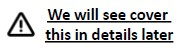
\includegraphics[scale=1]{img/cover.jpg}
    %\caption{}
\end{figure}

\tableofcontents
\newpage

{\Huge \textbf{Disclaimer}}\\ \\
Questa dispensa è stata prodotta traducendo e integrando le slide di lezione con gli appunti presi in aula e con i libri di testo consigliati durante l'a.a.2019-20. Sicuramente ci saranno errori/imprecisioni oppure i contenuti del corso potrebbero mutare di anno in anno. Consigliamo alle future generazioni di integrare/migliorare questa dispensa negli anni a venire e di diffonderla nuovamente una volta aggiornata.\\
Il codice sorgente LaTeX per modificarla è disponibile al seguente link:\\ \\
\texttt{inserire link di file sharing quando sarà pronto}

\newpage
\section{Introduzione}
\subsection{Storia del Modello Cloud}
Cloud Computing è un modello per consentire l’accesso a risorse condivise che possono essere fornite e rilasciate rapidamente e col minimo sforzo di gestione.\\
Il primo uso commerciale risale al 1970 con i Mainframes, grandi super computer installati in una stanza, erano molto costosi quindi difficilmente le compagnie ne avevano più di uno. L’accesso al Mainframe avveniva tramite terminali che erano solo in grado di trasferire dati in ingresso e in uscita. Si aveva quindi il problema del \textit{bottleneck} pertanto gli utenti dovevano aspettare a lungo per utilizzarlo.\\
Alla fine degli anni 70 abbiamo l'avvento dei PC. Le grandi organizzazioni installarono più PC in diversi uffici, funzionavano in maniera indipendente e per permettere la comunicazione tra di loro furono introdotte tecnologie per la comunicazione in rete (LAN e WAN).

\paragraph{Applicazioni Distribuite}
Gli approcci più classici sono:
\begin{itemize}
    \item \textbf{Client-Server,} in cui i ruoli sono predefiniti.
    \item \textbf{Peer-to-Peer,} in cui ogni computer può ricoprire sia il ruolo di client che di server.
\end{itemize}

\paragraph{Parallel Processing}
Originariamente si pensava che le prestazioni dei computer potessero migliorare solo producendo processori più veloci e potenti. Solo più tardi si capì che la soluzione migliore sarebbe stata utilizzare più processori che lavoravano insieme per risolvere un unico grande task. Ovviamente questo task deve essere progettato come composizione di task più piccoli che possano essere eseguiti in parallelo e questo fu possibile anche grazie ai notevoli miglioramenti della comunicazione in rete negli anni 80.

\begin{figure}[H]
    \centering
    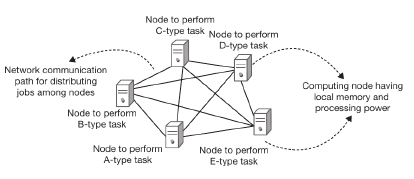
\includegraphics[scale=1]{img/pp.png}
    \caption{Modello Parallel Processing}
\end{figure}

\paragraph{Cluster Computing}
Il passo successivo è stata la creazione di cluster: gruppi di più nodi connessi con la stessa LAN per eseguire lo stesso task, o task simili. I computer vengono clusterizzati per una maggiore potenza di calcolo e per migliorare l’affidabilità. Tra i nodi di un cluster un nodo viene selezionato come \textit{cluster head} per supervisionare e distribuire i task tra i computer.
\begin{figure}[H]
    \centering
    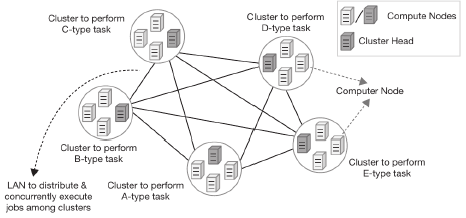
\includegraphics[scale=1]{img/cluster.png}
    \caption{Modello Cluster Computing}
\end{figure}

\paragraph{Grid Computing}
Il \textit{cluster head} poteva rappresentare un single point of failure pertanto, si passa dal Cluster al Grid Computing: un pool di risorse in cui le funzionalità di controllo sono implementate in maniera decentralizzata. I nodi potevano risiedere nella stessa rete o in aree differenti.

%%TABELLA PRO e CONTRO
\begin{table}[H]
    \begin{tabularx}{\linewidth}{>{\parskip1ex}X@{\kern4\tabcolsep}>{\parskip1ex}X}
    \toprule
    \hfil\bfseries Pro
    &
    \hfil\bfseries Contro
    \\\cmidrule(r{3\tabcolsep}){1-1}\cmidrule(l{-\tabcolsep}){2-2}
    
    %% PROS, seperated by empty line or \par
    Architettura scalabile che poteva fornire ottime performance per task complessi.\par
    &
    %% CONS, seperated by empty line or \par
    Non era possible real-time scaling.\par
    Il sistema non era Fault Tolerant.\par
    Hardware eterogenei richiedevano adattamento del codice.\par
    \\\bottomrule
    \end{tabularx}
\end{table}
\begin{figure}[H]
    \centering
    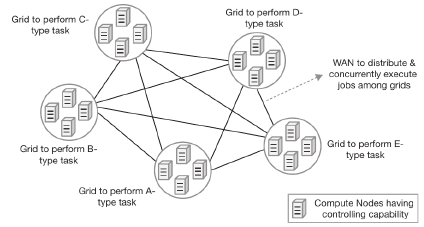
\includegraphics[scale=1]{img/grid.png}
    \caption{Modello Grid Computing}
\end{figure}
Agli inizi degli anni 90 grazie a nuove tecnologie si passò al Cloud computing.

\subsection{Servizi e Ruoli nel Cloud}
I servizi cloud sono implementati grazie alle risorse (RAM e CPU) fornite dalle cloud infrastructure, possono essere loro stessi un’applicazione o offrire un servizio.\\
Quando implementa un’applicazione solitamente espone un’interfaccia accessibile dalle pagine web, quando invece implementa un servizio sfruttato da altre applicazioni, queste accedono al servizio tramite interfacce API.  

\paragraph{XaaS - Everything as a Service}
I servizi cloud possono implementare una vasta gamma di funzioni, tutto può essere fornito come un servizio sfruttando questo paradigma. Alcuni esempi sono:
\begin{itemize}
    \item Casi in cui i file sono caricati nel cloud e da lì possono essere scaricati in altri dispositivi o condivisi con altri utenti. È possibile accedere al servizio tramite interfaccia web o app.
    \item ERP (Enterprise Resource Planning, un software usato dalle organizzazioni per gestire le attività commerciali) è locato nel cloud. I dipendenti lo accedono tramite un’interfaccia web da dovunque.
\end{itemize}

\paragraph{Ruoli}
\begin{figure}[H]
    \centering
    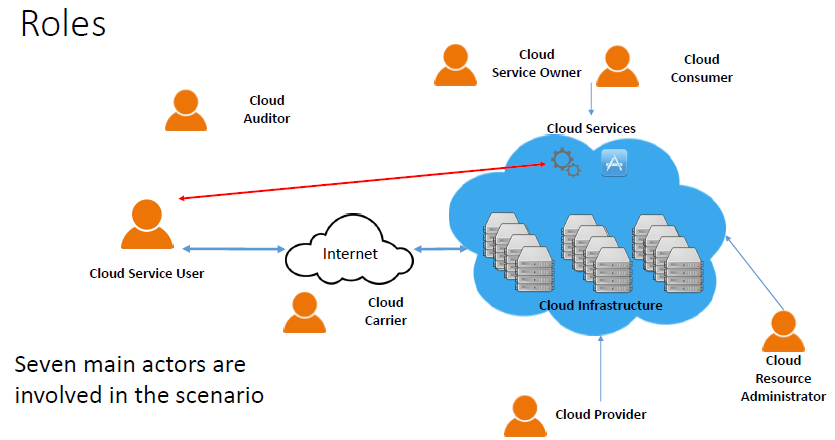
\includegraphics[scale=0.7]{img/roles.png}
    \caption{Principali attori in uno scenario Cloud}
\end{figure}
In uno scenario Cloud esistono diverse tipologie di ruoli:
\begin{itemize}
    \item\textbf{Cloud Provider:} organizzazione che fornisce le risorse, solitamente si occupa di creare e gestire la cloud infrastructure (es. Amazon, Google).
    \item \textbf{Cloud Consumer:} un’organizzazione o una persona che ha un contratto col cloud Provider per l’utilizzo delle risorse.
    \item \textbf{Cloud Service Owner:} un’organizzazione o una persona che crea un servizio cloud sfruttando le risorse fornite dal cloud infrastructure.
    \item \textbf{Cloud Resource Administrator: }un’organizzazione o una persona responsabile dell’amministrazione delle risorse. Solitamente appartiene al cloud provider.
    \item \textbf{Cloud Auditor:} una terza parte che conduce giudizi indipendenti sull’ambiente cloud, solitamente si occupa di valutare la sicurezza e le performance.
    \item \textbf{Cloud Carrier:} si occupa di fornire connettività tra gli utenti e il cloud provider.
    \item \textbf{Cloud Service User:} l’utente finale del servizio cloud.
    \item \textbf{Cloud Broker:} è un terzo che si interpone, in alcuni casi, tra il Cloud Provider e il Cloud Consumer: più specificatamente gestisce la distribuzione del servizio cloud da molteplici provider al consumatore negozia la relazione tra loro. In questo modo i consumatori posso evitare la responsabilità di interagire direttamente con il provider (interagendo solo con il broker) e posso beneficiare di una riduzione dei costi, richiedendo servizi da più provider contemporaneamente.
\end{itemize}
Il modello Cloud si basa sulle risorse offerte dal cloud provider, il modello è scalabile e misurato, questo comporta due caratteristiche principali:
\begin{itemize}
    \item Adotta un utility-based model: paghi per quello che usi (l’uso delle risorse viene “misurato”).
    \item Le risorse possono essere assegnate dinamicamente su richiesta (sia a persone fisiche che ai software direttamente).
\end{itemize}
Le risorse devono essere instanziate dal cloud provider velocemente e vengono gestite col minimo sforzo, senza l’intervento umano; i consumer le possono accedere contemporaneamente via internet. L’infrastruttura cloud è locata nei data center, spazi dedicati per ospitare server e apparecchiature di rete, dal cloud provider.

\subparagraph{Multi-Tenancy}
Le tradizionali strutture informatiche sono multi-users permettendo a più utenti di accedere alle risorse del sistema, se il numero di utenti diventa troppo grande per l’amministratore diventa impossibile gestire tutte le richieste.\\
Le strutture informatiche cloud sono multi-tenant, i tenant non sono utenti normali ma sono gli amministratori dei rispettivi sistemi, per far sì che siano scalabili vogliamo che i consumer abbiano l’impressione di avere il totale controllo delle risorse che gli sono state assegnate.\\
Per creare una struttura multi-tenant la chiave è la \textit{virtualizzazione} (ne parleremo più avanti nel dettaglio).

\newpage
\subsection{Benefici}
Il calcolo via cloud ha radicalmente cambiato il modo in cui i sistemi IT vengono progettati e implementati, andando a introdurre un reale cambiamento di paradigma. A differenza dei convenzionali paradigmi di calcolo, fornisce un gran numero di vantaggi sul fronte business. La tecnologia e le relative opportunità hanno cambiato il modo in cui le aziende si organizzano, ha inoltre aperto la strada a nuove possibili strategie e opportunità che prima erano impensabili.\\
Le soluzioni di calcolo tradizionali per l’implementazione di servizi aziendali (business), richiedono solitamente la progettazione e l’implementazione di una completa infrastruttura IT costruita e mantenuta direttamente presso le proprie sedi. Questo può avvenire con un investimento iniziale significativo, sia per quanto riguarda l’hardware da piazzare che di personale addetto alla manutenzione. Per quanto riguarda il personale, nel sopracitato contesto, è richiesto di riservarne una parte per progettare e mantenere tutti gli aspetti del sistema del Sistema Operativo al Networking. Questo processo richiede un workflow particolare:\\

\begin{center}
% Define block styles
\tikzstyle{block} = [rectangle, draw, 
    text width=10em, text badly centered, rounded corners, minimum height=4em]
\tikzstyle{line} = [draw, -latex']
\begin{tikzpicture}[node distance = 3cm, auto]
    % Place nodes
    \node [block] (1) {Comprare \& installare hardware};
    \node [block, right of=1, node distance=5cm] (2) {Installare \& configurare il SO e l'equipaggiamento di rete};
    \node [block, right of=2, node distance=5cm] (3) {Installare il software e costruire il servizio};

    % Draw edges
    \path [line] (1) -- (2);
    \path [line] (2) -- (3);
\end{tikzpicture}
\end{center}
Dopo aver completato la realizzazione del sistema, un altro significativo sforzo deve essere compiuto per tenerlo attivo e farlo girare senza difficoltà; anche questo task richiede un impegno addizionale significativo di personale, direttamente nella sede. Tutto questo si riflette in bilancio con costi fissi di personale e riparazioni hardware. In particolare, la compagnia ha bisogno di accollarsi i seguenti tasks:
\begin{itemize}
    \item Riparazione di Hardware fallato e sostituzione di Hardware vecchio.
    \item Aggiornamento del sistema operativo e applicazione di patch di sicurezza.
    \item Mantenere tutto l’ambiente software.
\end{itemize}
Nel frattempo, però, l’azienda può crescere (pure in maniera inaspettata, addirittura in una nottata in qualche caso particolare), quindi il sistema deve essere pronto a scalare per poter gestire una richiesta crescente. Quindi, l’hardware esistente deve essere aggiornato, acquistando e installando risorse o hardware addizionali in modo da gestire il carico. Questo ovviamente comporta un costo addizionale. Però allo stesso modo in cui l’azienda cresce, si potrebbero anche verificare dei casi di calo drastico di business, sia in maniera permanente che temporanea. In questo caso, il carico si riduce e il sistema non può essere scalato, dato che le risorse che sono state precedentemente acquistate non possono essere disinstallate e vendute. Si verifica quindi uno spreco di risorse, dato che le risorse installate non vengono utilizzate.\\
In questo caso, quindi, il “Cloud Computing” con il suo paradigma basato sull’utilità, può essere estremamente utile. Il termine “servizio di utilità” si associa ad un tipo di servizio on-demand e controllato che si riflette in un modello “pay-per-use”, ottenendo risorse di calcolo in maniera proporzionale al carico. Consente quindi di introdurre scalabilità dinamica, di ridurre i costi sia iniziali che operativi.\\
I principali benefici che se ne possono trarre, sono i seguenti:
\begin{itemize}
    \item \textbf{Scalabilità:} la misura del servizio, si può basare sulle attuali richieste. Tale approvvigionamento dinamico, può essere fatto automaticamente utilizzando software di automazione. Questo aggiunge la possibilità di espandere o ridurre dinamicamente le risorse associate a un servizio.
    \item \textbf{No costi fissi:} i servizi possono essere creati anche senza possedere un’infrastruttura di calcolo o risorse IT. Quindi, non è necessario un investimento iniziale e non c’è bisogno di costi di manutenzione, in quanto non c’è bisogno di mantenere personale specializzato per gestire l’infrastruttura.
    \item \textbf{Riduzione costi:} i gestori di “Cloud Computing”, in generale, offrono risorse IT ad un costo veramente basso. Questo può essere garantito andando a creare un’infrastruttura con le seguenti caratteristiche:
    \begin{itemize}
        \item Larga: comprando hardware IT in stock si vanno a ridurre i costi.
        \item Condivisa: clienti differenti condividono la stessa infrastruttura, quindi le risorse sono tutte pienamente sfruttate andando ad eliminare i periodi morti.
        \item Costi fissi condivisi: le conoscenze sono condivise tra tutto il personale, di conseguenza anche i costi relativi sono molto ridotti.
    \end{itemize}
\end{itemize}
I vantaggi del Cloud Computing possono essere comparati a quelli di tutti i sistemi di utilità. Quindi, per esempio, il ragionamento è lo stesso di un approvvigionamento di energia elettrica, in cui, ovviamente, conviene acquistare energia piuttosto che prodursela da soli.\\ 
Ci sono, però, altri vantaggi indiretti in questo approccio che possono essere riassunti come segue:
\begin{itemize}
    \item \textbf{Minima responsabilità manageriale:} gestire l’infrastruttura IT è una responsabilità per la compagnia, anche dal punto di vista legale. Il Cloud invece, sposta la maggior parte dei task relativi alla gestione dell’infrastruttura direttamente al provider, che con team dedicati si prendono cura di tutte queste attività.
    \item \textbf{Più alta qualità del servizio:} nelle imprese di computing tradizionale, l’infrastruttura era gestita da un team che non era completamente concentrato su questo tipo di task o, addirittura, scaricato a terze parti. La qualità dell’infrastruttura, quindi, era strettamente legata all’esperienza del team o delle terze parti e dipendente, inoltre, dall’ammontare di task addizionali che avevano. Mentre, i provider di Cloud Computing hanno team dedicati di esperti che sono completamente concentrati a garantire un’alta qualità del servizio.
    \item \textbf{Affidabilità:} l’alta qualità del management aiuta ad aumentare l’affidabilità in maniera significativa. L’adozione di tecniche per alta disponibilità, come il bilanciamento del carico, backup e procedure di recupero consentono di garantire massima affidabilità o veloci recuperi da fallimenti hardware. I clienti, quindi, non hanno più bisogno di prendersi cura di questi problemi, dato che il provider del servizio si prende cura di creare un ambiente che sia sicuro da fallimenti hardware o disastri in generale.
    \item \textbf{Gestione minima del software:} task fondamentali nella creazione di un’infrastruttura IT riguardano l’acquisto di licenze e gestione del software. Nel Cloud Computing, in alcuni dei suoi tipi di servizi, si prende cura non solo dell’infrastruttura in generale, ma anche del software. Questo elimina la fase di acquisto di licenze (dato che questo compito passa completamente al provider cloud) e, soprattutto, di gestione del software come aggiornamenti e patch.
    \item \textbf{Indipendenza dal luogo:} i servizi cloud sono acceduti via Internet. Questo significa che tali servizi possono essere acceduti da qualsiasi luogo, in qualsiasi momento.
    \item \textbf{Le compagnie possono concentrarsi sui loro business:} i developers delle aziende, possono quindi concentrarsi sull’implementazione della logica del business piuttosto che sul mantenimento dell’infrastruttura.
\end{itemize}
I vantaggi relativi al Cloud Computing stanno portando ad una “cloudificazione”, termine coniato per riferirsi al fenomeno di spostamento di applicazioni e servizi da deployments locali di calcolo ad un luogo non ben definito, nel cloud. Quindi, le infrastrutture locali sono dismesse per spostare i servizi e le applicazioni in cloud.\\
Compagnie che richiedono sporadicamente capacità di calcolo ad alte performance (HPC – High Performance Computing), per un periodo di tempo veramente breve, possono noleggiare un grande ammontare di risorse senza mantenere una propria infrastruttura. Questo è il caso d’uso, ad esempio, della Pixar, che noleggia le infrastrutture necessarie al rendering dei propri film soltanto nel periodo in cui gli è necessario per la realizzazione. \\
Con i convenzionali paradigmi di calcolo sarebbe impossibile implementare e far girare un servizio su scala globale, in cui miliardi di utenti che si collegano contemporaneamente. Questo perché implementare un servizio su scala globale in un’unica location porterà a problemi di scalabilità, visto che i dati devono essere trasferiti in tutto il globo attraverso internet, portando a bottleneck ed alta latenza. I dati relativi ad un tale sistema, inoltre, richiedono soluzioni ad-hoc di storage, che difficilmente possono essere implementati in un singolo luogo. Un’azienda, quindi, per ovviare a questo problema dovrebbe andare a costruire differenti infrastrutture IT in differenti luoghi (ad esempio uno per ogni continente o nazione) per avere istanze multiple del servizio Cloud per girare le richieste degli utenti al server più vicino. Quindi, il servizio dovrebbe essere re-ingegnerizzato per spargere i dati (in questo caso in grande quantità) su luoghi multipli e distribuire lo sforzo computazionale. Questa cosa viene fatta dai provider di servizi cloud, ovvero le loro infrastrutture vengono divise in diversi datacenter piazzati in tutto il mondo per coprire efficientemente varie aree e offrendo ai clienti soluzioni ad-hoc per replicare i servizi cloud su differenti data center.\\
Nonostante i vantaggi appena descritti, l’approccio cloud comunque potrebbe avere degli svantaggi, quando si fa una comparazione con un approccio tradizionale. Questi svantaggi rappresentano da un lato dei challenge per i provider dei servizi cloud per supportare una più vasta gamma di casi d’uso e dall’altro, rischi per i clienti di tale servizio:
\begin{itemize}
    \item \textbf{Costi di network:} il Cloud Computing richiede una costante connettività per accedere al servizio. Questo introduce un costo non trascurabile per mantenere una certa banda.
    \item \textbf{Banda del network (bottleneck):} nonostante il costo dell’accesso al network possa essere accessibile, la banda potrebbe comunque essere limitata. Quando si ha a che fare con applicazioni che gestiscono un grande ammontare di dati critici, il network stesso potrebbe rappresentare un bottleneck, andando quindi a limitare i vantaggi dei servizi cloud.
    \item \textbf{Limitata portabilità:} la standardizzazione delle tecnologie cloud è ancora limitata. Siamo quindi lontani dall’avere uno standard diffuso e ben riconosciuto. Quindi, differenti provider hanno differenti soluzioni che sono proprietarie e che quindi non sono in grado di cooperare o integrarsi. Un servizio, implementato su una certa infrastruttura di un certo provider cloud, difficilmente potrà essere esportato su una differente infrastruttura. Quindi, ogni provider sostanzialmente “blocca” la possibilità di portabilità delle applicazioni cloud. 
    \item \textbf{Problemi legali:} i provider di Cloud Computing costruiscono i propri data center in luoghi di loro convenienza, sia dal punto di vista geografico che economico. La location designata per lo storage dei dati dei clienti del cloud potrebbe essere al di fuori del loro stato o regione. Dato che le leggi sulla privacy o conformità differiscono da stato a stato, possono presentarsi problemi legali a riguardo. Per esempio, alcuni stati richiedono che i dati sensibili (per esempio medici) siano salvati nello stesso stato dell’utente, quindi questo potrebbe portare a problemi legali quando sono coinvolti dati di questo tipo.
\end{itemize}
Nell’ambito del Cloud Computing, utenti e aziende hanno bisogno di salvare i propri dati all’esterno dei confini della propria organizzazione. I dati sono trasmessi attraverso un network che potenzialmente non può essere considerato affidabile, i dati sono salvati in infrastrutture del provider che sono tipicamente considerate affidabili. Sono coinvolti quindi differenti confini di affidabilità e credibilità, a differenza dell’approccio tradizionale in cui tutto avveniva all’interno dei confini dell’azienda stessa. La trasmissione di dati su di un network non considerato affidabile, richiede il coinvolgimento di meccanismi di sicurezza, come ad esempio criptare i dati stessi. Quindi, costruire una confidenza per i consumatori riguardo la sicurezza dei dati salvati all’esterno dei confini del proprio network è un grande challenge per i provider cloud.  

\newpage
\subsection{Modelli NIST e di Erogazione dei Servizi}
La standardizzazione del Cloud Computing è limitata, in quanto è una tecnologia introdotta recentemente e ancora nuova. Ogni cloud provider adotta la propria soluzione tecnologica per il suo servizio.\\
Come per ogni tecnologia, abbiamo bisogno di un modello standard per comodità di comprensione. Inizialmente, sono stati definiti molti modelli per cloud computing in modo da standardizzare gli aspetti di questa tecnologia e tra questi abbiamo un modello definito dal National Institute of Standard and Technology (NIST). Questo modello pubblicato nel ‘NIST Cloud Computing Reference Architecture’ è il più apprezzato e accettato. Esso definisce un modello che fornisce una definizione di cloud computing e un’architettura di riferimento.\\
Il NIST model definisce gli aspetti e le caratteristiche base del cloud computing:
\begin{itemize}
    \item \textbf{Caratteristiche Essenziali:} il set di feature mandatorie che ogni sistema di cloud computing deve avere.
    \item \textbf{Modelli di Servizio:} il set dei diversi tipi di servizi che vengono forniti ai consumatori.
    \item \textbf{Modelli di Implementazione:} il set dei modelli per l’implementazione dell’infrastruttura cloud.
\end{itemize}
Il modello NIST include cinque caratteristiche essenziali per l’infrastruttura:
\begin{itemize}
    \item \textbf{Broad Network Access:} l’infrastruttura deve essere accessibile da ovunque.
    \item \textbf{Rapid Elasticity}: le risorse vengono allocate/deallocate rapidamente.
    \item \textbf{Measured Service:} le risorse sono misurabili e prezzate proporzionalmente al loro uso.
    \item \textbf{On-Demand:} le risorse vengono allocate su richiesta.
    \item \textbf{Resource Pooling:} Il pool delle risorse di computazione, da allocare su richiesta dei clienti, viene mantenuto in remoto e deve essere abbastanza grande da soddisfare molti utenti simultaneamente.
\end{itemize}
L’implementazione dell’infrastruttura cloud e dei servizi corrispondenti può essere organizzata in diversi modi, dipendentemente dai requisiti dell’organizzazione del cliente: i diversi modelli sono correlati alla posizione dell’infrastruttura rispetto all’organizzazione.\\
Il modello NIST definisce quattro tipi di implementazione:
\begin{itemize}
    \item \textbf{Public Cloud:} (o External Cloud) è il modello piú popolare. In questo modello l’infrastruttura è gestita da un’organizzazione esterna che vende il servizio e le risorse. Nel Public Cloud l’utente accede al servizio da remoto, in quanto l’infrastruttura è posizionata fuori sede rispetto all’organizzazione del consumatore.\\ Il Public Cloud promuove la \textit{multi-tenancy} al suo massimo livello: le stesse risorse fisiche sono condivise tra un grande numero di utenti indipendenti tra loro. In questo modo il provider può mantenere costi ridotti e permettersi tecnologie all’avanguardia e personale qualificato.
    \item \textbf{Private Cloud:} sviluppate e gestite da una sola organizzazione per il proprio utilizzo interno (accesso limitato).\\ Una Private Cloud solitamente risiede all’interno dei locali dell’organizzazione del cliente o all’esterno in una locazione neutrale. In ogni caso, la sua gestione è responsabilità del cliente o di una compagnia esterna di fiducia. Questo modello di solito viene adottato quando il consumatore desidera un controllo specifico sull’ambiente o ci sono dei requisiti specifici.
    \item \textbf{Community Cloud:} permettono ad un certo numero di organizzazioni o clienti che appartengono a una community. Esse sono costruite e gestite dalla stessa community di persone o organizzazioni che hanno interessi e obiettivi comuni. Di conseguenza, queste implementazioni sono aperte solo ai membri della community correlata. Come per le implementazioni private, esse possono risiedere sia in locale che all’esterno e possono essere gestite dalla community stessa o da un fornitore esterno.\\ Questo genere di implementazione è una forma di Private Cloud generalizzata: il modello supporta la multi-tenancy tra i membri della community, in modo da fornire i benefici del Public Cloud unito al controllo del modello privato.\\ In questo modello i costi sono condivisi tra tutti i membri della community, quindi sono più bassi rispetto al modello Public Cloud. Inoltre, il modello pay-per-use può essere applicato.
    \item \textbf{Hybrid Cloud:} creato combinando un’infrastruttura private con un’infrastruttura public. In questo modo il cliente potrà avere sia i vantaggi dell’implementazione pubblica (risorse computazionali a basso costo e alta scalabilità) e dell’implementazione privata (alto livello di controllo sull’infrastruttura e privacy dei dati). I servizi possono essere sviluppati sia sulla parte pubblica, che su quella privata o su entrambe.
\end{itemize}
La scelta del modello più appropriato del modello dipende dai requisiti di business e dalla taglia dell’organizzazione cliente. Per un utilizzo generale qualunque Public Cloud è una buona opzione, mentre le diventano un’opzione quando la compagnia ha bisogni particolari sulla privacy dei dati o se gestisce un business con dati sensibili.

\paragraph{Modelli di Erogazione del Servizio Cloud}
Il modello NIST definisce tre principali modelli di erogazione del servizio, dipendentemente dal tipo di servizio offerto ai clienti e da come viene fornito: \textit{IaaS, Paas} e \textit{SaaS}.\\
Questi modelli di erogazione sono ben stabiliti al giorno d’oggi e offerti da quasi ogni cloud provider sul mercato. I diversi tipi di modelli si distinguono tra loro per il livello di astrazione dall’infrastruttura hardware.

\subsubsection{IaaS - Infrastructure as a Service}
Consegna ai clienti le risorse hardware virtualizzate e fornisce la possibilità di utilizzare da remoto le risorse computazionali virtuali. Queste risorse possono essere usate come fossero hardware reale per creare qualsiasi VM.

\begin{figure}[H]
    \centering
    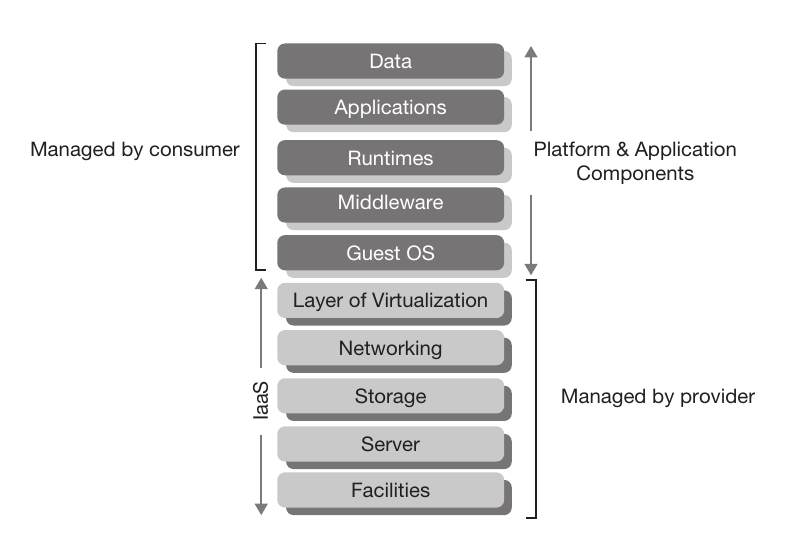
\includegraphics[scale=0.5]{img/iaas.png}
    \caption{Modello IaaS}
\end{figure}
\noindent
Il consumatore non deve più gestire e controllare l’infrastruttura computazionale che è, invece, gestita dal provider: deve però continuare a prendersi cura delle componenti di piattaforma e applicazione (Installazione OS, middleware software, sviluppo dell’applicazione e gestione dati).\\
IaaS rimuove i costi di costruzione e mantenimento di una infrastruttura fisica, con un buon controllo dell’ambiente dove sviluppare i servizi.

\subsubsection{PaaS - Platform as a Service}
Fornisce ai consumatori l’accesso a una piattaforma in cui essi possono progettare e sviluppare le componenti delle applicazioni.\\
Il consumatore deve occuparsi solo della programmazione del livello applicazione e della gestione dei dati, gli altri aspetti dall’infrastruttura fisica alla piattaforma middleware verranno gestite dal provider.
\begin{figure}[H]
    \centering
    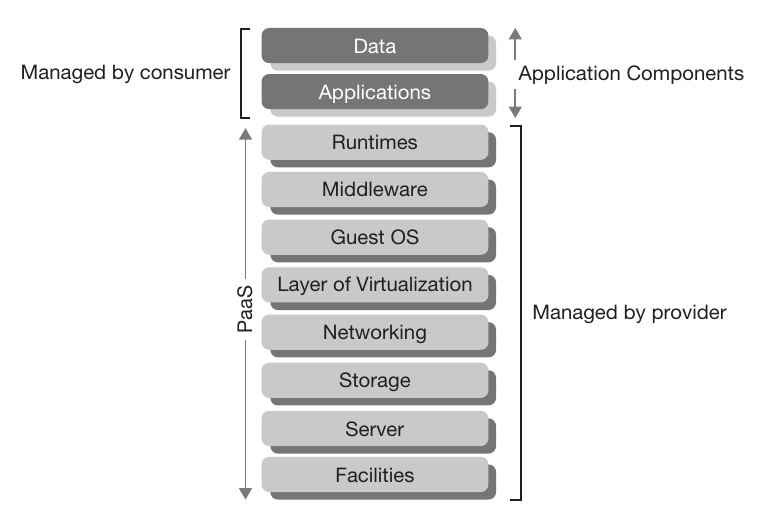
\includegraphics[scale=0.5]{img/paas.png}
    \caption{Modello PaaS}
\end{figure}
\noindent
Il consumatore sviluppa la sua logica applicativa all’interno dell’ambiente di programmazione fornito dal provider. Il grande svantaggio di questo approccio è la mancanza di flessibilità: le applicazioni devono essere programmate con le API fornite dal sistema e le applicazioni cosi programmate sono quindi difficilmente portabili da una piattaforma cloud a un’altra.

\subsubsection{SaaS - Software as a Service}
Il provider consegna come servizio ai clienti direttamente delle applicazioni. Queste applicazioni sono sviluppate dal provider e solitamente offerte ai consumatori attraverso un’interfaccia web.
\begin{figure}[H]
    \centering
    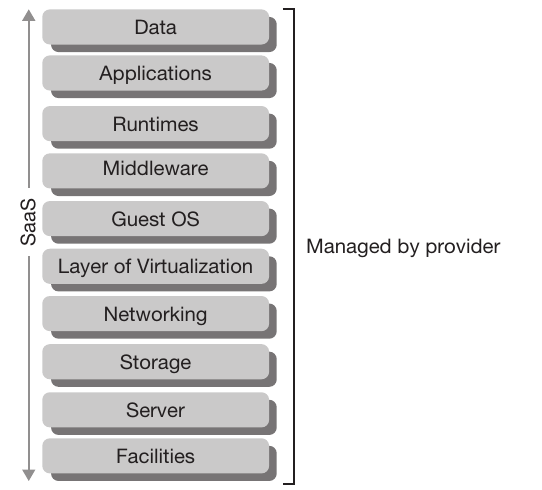
\includegraphics[scale=0.5]{img/saas.png}
    \caption{Modello SaaS}
\end{figure}
\noindent
In questo modello il cloud provider gestisce tutti gli aspetti del sistema, dall’hardware al software, e il consumatore non deve occuparsi di nulla.\\

\paragraph{Integrazione}
I tre modelli base precedenti possono essere composti insieme:
\begin{itemize}
    \item PaaS e SaaS possono essere implementati al di sopra di un’infrastruttura IaaS
    \item Un’infrastruttura IaaS può essere usata per creare un’infrastruttura PaaS: vengono create macchine virtuali su cui è installata una piattaforma software
    \item Un’infrastruttura PaaS può essere usata per creare un sistema SaaS: una piattaforma PaaS utilizzata per creare un software che viene fornito come SaaS
\end{itemize}
Esistono anche altri servizio cloud. Ne elenchiamo alcuni:
\begin{itemize}
    \item Storage as a Service
    \item Database as a Service
    \item Backup as a Service
    \item Desktop as a Service
\end{itemize}

\newpage
\section{Tecnologie di Virtualizzazione}
\subsection{Introduzione}
L'esecuzione simultanea di più computer virtuali su un singolo set di risorse fisiche offre grandi vantaggi in termini di utilizzo ottimale delle risorse, rendendo un sistema dinamico, e migliorando la sicurezza attraverso l'astrazione delle risorse. \\ 
Un modulo software chiamato \textbf{hypervisor} gioca un ruolo fondamentale nella virtualizzazione. \\
Con la virtualizzazione si va a rappresentare le risorse di elaborazione fisica in forma simulata attraverso un livello software aggiuntivo. Ci riferiremo a questo livello software aggiuntivo come layer of virtualization. Questo livello trasforma le risorse di elaborazione fisica in forma virtuale che gli utenti utilizzano per soddisfare le loro esigenze di elaborazione. \\
La figura sottostante rappresenta il concetto base di virtualizzazione in una forma semplificata. 
\begin{figure}[H]
    \centering
    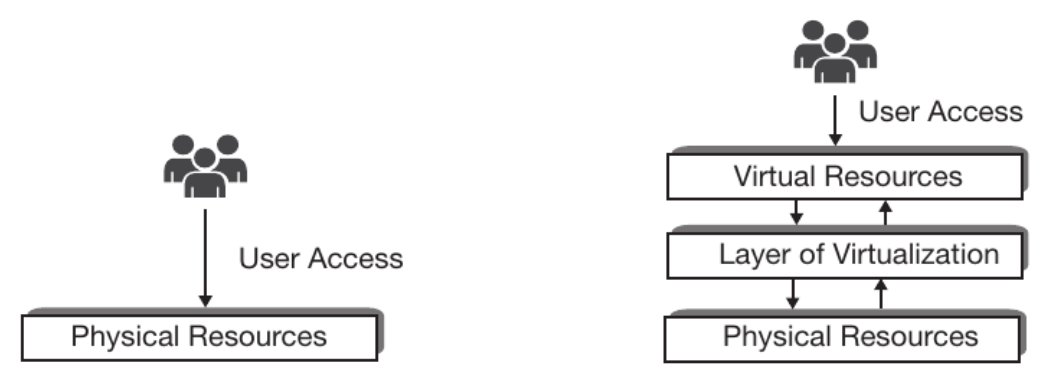
\includegraphics[scale=0.5]{img/virtualization technologies.png}
    \caption{Modello di virtualizzazioni}
\end{figure}\noindent
In parole povere, la virtualizzazione è la separazione logica delle risorse fisiche che fa sì che gli utenti non possano accedervi direttamente per soddisfare le loro esigenze anche se, alla fine, le risorse fisiche sono coloro che forniranno i servizi richiesti. Quindi la virtualizzazione è colei che andrà a fornire un livello di astrazione logica. \\
L'astrazione è il processo che nasconde le caratteristiche complesse e non essenziali di un sistema. Attraverso l'astrazione, un sistema può essere presentato in modo semplificato per un uso particolare nascondendo agli utenti dettagli indesiderati. Nell'informatica, l'astrazione viene implementata attraverso gli strati del software. Lo strato del sistema operativo può essere trattato come uno strato di astrazione. \\
Nel cloud computing la virtualizzazione delle risorse (che aggiunge uno strato software alle risorse di elaborazione fisica per creare risorse virtuali) funge da strato di astrazione. La sua astrazione rende più facile offrire un servizio più flessibile, affidabile e potente. \\
Ogni tipo di risorsa IT può essere virtualizzata: dai dispositivi base (processore, RAM, ecc) ad altre risorse come la memoria, dispositivi network o periferiche (tastiere, mouse, stampanti, ecc). Tuttavia, va notato che nel caso delle risorse di elaborazione di base un componente virtualizzato può essere operativo solo quando una risorsa fisica lo abilita dal back-end. Ad esempio, un processore virtuale può funzionare solo quando è collegato un processore fisico. \\
La cosa importante da notare è che i dispositivi simulati prodotti attraverso la virtualizzazione possono o meno assomigliare ai componenti fisici reali (in termini di qualità, architettura o quantità). Ad esempio, nella figura sotto riportata, gli utenti hanno accesso a tre processori mentre in realtà esiste un processore fisico. Oppure, il processore a 32 bit può essere prodotto (in forma virtuale) dal processore fisico effettivo a 64 bit.
\begin{figure}[H]
    \centering
    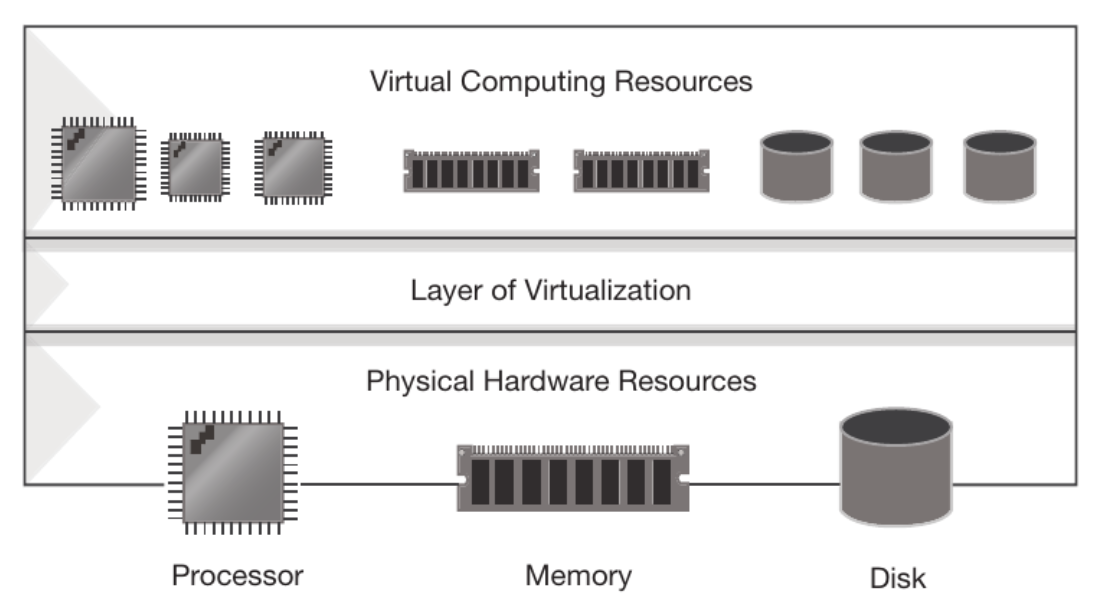
\includegraphics[scale=0.5]{img/resource virtualization.png}
    \caption{Virtualizzazione delle risorse}
\end{figure}\noindent
La virtualizzazione migliora radicalmente la flessibilità e la disponibilità delle risorse informatiche e le organizzazioni possono guadagnare in termini di business. Esistono diversi tipi di tecnologie di virtualizzazione come il Server virtualization, Storage virtualization, Network Virtualization ecc. Tra questi, il fattore principale che guida il passaggio alla virtualizzazione è il Server virtualization, che è la parte più importante della tecnologia di virtualizzazione delle risorse di elaborazione. \\
Il \textbf{Machine/Server virtualization} è il concetto di creare una macchina virtuale (o un server virtuale) nella attuale macchina fisica. La macchina fisica è chiamata \textbf{host system} e la macchina virtuale \textbf{guest system}. Nel sistema informatico convenzionale, c'è sempre stata una relazione uno a uno tra computer fisico e sistema operativo. Uno alla volta, un singolo sistema operativo può essere eseguito su di esso. \\
La virtualizzazione dell'hardware elimina la limitazione di avere una relazione uno a uno tra hardware fisico e sistema operativo. Facilita il funzionamento di più sistemi informatici con i propri sistemi operativi su una singola macchina fisica. Come mostrato nella figura sottostante, il sistema operativo dei sistemi guest in esecuzione sulla stessa macchina fisica non deve essere simile. Tutte queste macchine virtuali in esecuzione su un singolo sistema host, rimangono indipendenti l'una dall'altra. I sistemi operativi sono installati in quelle macchine virtuali. I guest systems possono accedere all'hardware del host system e possono eseguire le applicazioni all'interno del proprio ambiente operativo. 
\begin{figure}[H]
    \centering
    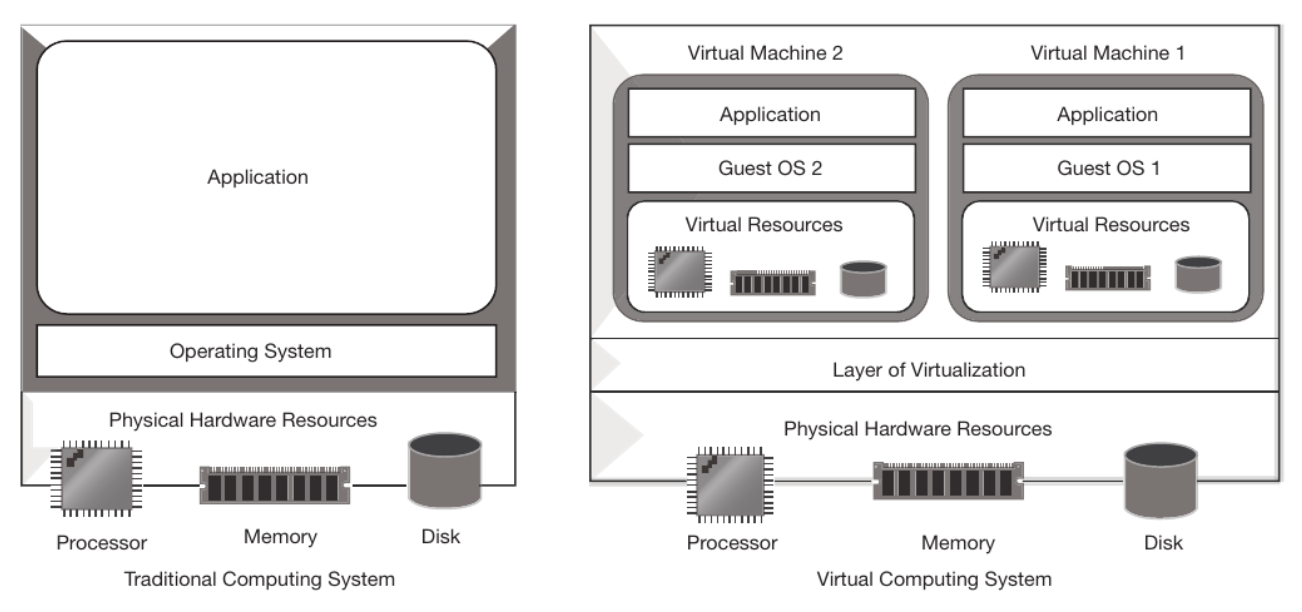
\includegraphics[scale=0.5]{img/machine-server virtualizzation.png}
    \caption{Virtualizzazione macchina/server}
\end{figure}\noindent
Nella tabella sono riportate le differenze tra \textit{Non-Virtualized Machine Environment} e \textit{Virtualized Machine Environment}. \\
\begin{table}[H]
    \begin{tabularx}{\linewidth}{X | X}
    \hline
    \textbf{Non-Virtualized Machine Environment} & \textbf{Virtualized Machine Environment}\\ [0.5ex]
    \hline\hline
    Un singolo OS può girare su una macchina fisica alla volta &
    Più OS possono girare simultaneamente su una macchina fisica \\
    \hline
    Il sistema applicativo e hardware rimane strettamente accoppiato &
    La VM isola le applicazioni dal livello hardware sottostante \\
    \hline
    Il rate di utilizzo delle risorse è basso il più delle volte & 
    L'utilizzo delle risorse migliora dato che più VM condividono lo stesso set di risorse fisiche \\
    \hline
    I costi di business aumentano a causa del basso utilizzo delle risorse & Se pianificati correttamente sono convenienti \\
    \hline
    Hanno un approccio non flessibile & 
    Forniscono molta flessibilità ai system designers\\ [1ex] 
    \hline
    \end{tabularx}
\end{table}
Le VM vengono create sopra ai livelli di virtualizzazione. Questo livello di virtualizzazione:
\begin{itemize}
    \item È un insieme di programmi di controllo che creano l'ambiente per l'esecuzione delle VM.
    \item Fornisce alle VM l'accesso alle risorse di sistema.
    \item Controlla e monitora l'esecuzione delle VM su di esse. 
\end{itemize}
Questo livello software è chiamato \textit{Hypervisor} o \textbf{Virtual Machine Monitor} (VMM). Il VMM crea una astrazione del livello software e/o hardware sottostante e rappresenta le risorse del sistema virtuale per i suoi utenti. Questo livello facilita anche l’esistenza di più macchine virtuali che non sono obbligate a condividere lo stesso kernel del sistema operativo (sottostante). Per questo motivo diventa possibile eseguire diversi sistemi operativi sulle macchine virtuali che sono state create sopra ad un VMM. Il VMM fornisce una console di sistema amministrativa attraverso la quale è possibile gestire l’ambiente del sistema virtuale (come il numero di componenti virtuali o la capacità dei vari componenti). \\
Le tecniche di virtualizzazione che si basano sul VMM possono essere suddivise in tre categorie: \textit{Full virtualization}, \textit{Para-virtualization} e \textit{Hardware-assisted virtualization}.

Esistono due diverse tipologie di Hypervisor: l’\textit{hosted approach} e il \textit{bare metal approach}. Sebbene le tecniche siano diverse hanno lo stesso obiettivo finale, creare una piattaforma in cui più macchine virtuali possono condividere le stesse risorse di sistema. Ogni tecnica è semplicemente un modo diverso di raggiungere questo obiettivo.

\paragraph{Meccanismo \textit{Trap-and-Emulate}}
Meccanismo tramite il quale vengono intercettate delle interruzioni/eccezioni o comunque operazioni che non possono essere eseguite da un guest OS. Le trap sono usate dall'Hypervisor per intercettare queste chiamate, eseguirle al posto della VM e, alla fine, fornire al guest OS i dati come se avesse eseguito esso stesso il codice.
Lo svantaggio principale è l'overhead generato a causa del dover emulare le istruzioni.

\subsubsection{Hosted Approach}
In questo approccio, un sistema operativo viene prima installato sulla macchina fisica per poterlo attivare. Il sistema operativo installato sul computer host viene definito \textit{\textbf{host operating system}}. L'hypervisor viene quindi installato su questo host OS. Questo tipo di hypervisor viene definito \textit{\textbf{hypervisor di tipo 2}} o \textit{\textbf{hosted hypervisor}}. La figura sottostante rappresenta la tecnica di virtualizzazione dell’hosted machine.
\begin{figure}[H]
    \centering
    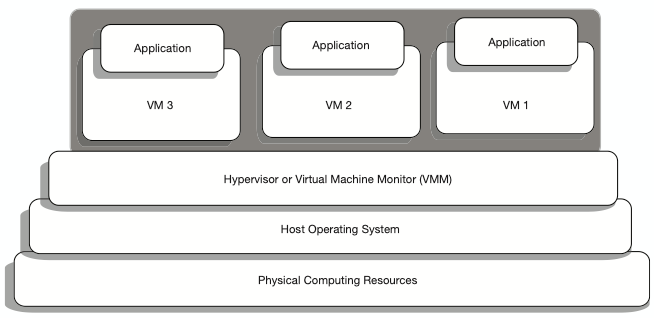
\includegraphics[scale=0.8]{img/hosted approach.png}
    \caption{Hosted Approach}
\end{figure}\noindent
\uline{Vantaggi:} in questo approccio l’host OS fornisce i driver hardware per le risorse fisiche sottostanti. Facilita l'installazione e la configurazione dell'hypervisor. Rende gli hypervisors di tipo 2 compatibili per un'ampia varietà di piattaforme hardware. \\
\uline{Svantaggi:} un hosted hypervisor non ha accesso diretto alle risorse hardware e, quindi, tutte le richieste dalle macchine virtuali devono passare attraverso l’host OS. Questo potrebbe peggiorare le prestazioni delle macchine virtuali. Un altro svantaggio dell’hosted virtualization è la mancanza di supporto per i sistemi operativi in tempo reale. Poiché l’host OS sottostante controlla la pianificazione dei lavori, diventa irrealistico eseguire un OS in tempo reale all'interno di una macchina virtuale utilizzando l’hosted virtualization.

\subsubsection{Bare Metal Approach Rimozione dell'Host OS}
In questo approccio l'hypervisor viene installato direttamente sulla macchina fisica. Poiché l'hypervisor è il primo livello rispetto alle risorse hardware la tecnica viene definita approccio \textit{bare metal}. Qui, il VMM o hypervisor comunicano direttamente con l'hardware del sistema. \\
In questo approccio, l'hypervisor funge da monitor per le macchine virtuali di basso livello e viene anche chiamato \textit{\textbf{hypervisor di tipo 1 o native hypervisor}}. I server ESX ed ESXi di VMware, Hyper-V di Microsoft e la soluzione Xen sono alcuni degli esempi di bare metal hypervisors. \\ 
\uline{Vantaggi:} poiché il bare metal hypervisor può accedere direttamente alle risorse hardware, nella maggior parte dei casi offre prestazioni migliori rispetto all'hosted hypervisor. Per applicazioni più grandi come i data center aziendali, la virtualizzazione bare metal è più adatta perché di solito fornisce funzionalità avanzate per la gestione delle risorse e della sicurezza. Gli amministratori ottengono un maggiore controllo sull'ambiente host. \\
\uline{Svantaggi:} come ogni hypervisor di solito ha un set limitato di device drivers integrati, quindi i bare metal hypervisor hanno un supporto hardware limitato e non possono essere eseguiti su un'ampia varietà di piattaforme hardware.
\begin{figure}[H]
    \centering
    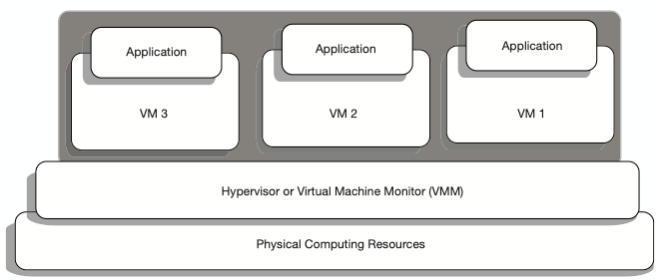
\includegraphics[scale=0.8]{img/bare metal.png}
    \caption{Bare Metal Approach}
\end{figure}\noindent

\subsubsection{Full Virtualization}
Nella \textit{full virtualization} (chiamata anche \textit{native virtualization}), l'hypervisor simula o emula completamente l'hardware sottostante. Le macchine virtuali vengono eseguite su questo set di hardware virtuale. I guest OS pensano che siano in esecuzione su risorse fisiche effettive e quindi rimangono inconsapevoli di essere stati virtualizzati. \uline{Questo consente alle versioni non modificate dei sistemi operativi} (come Windows, Linux e altri) \uline{di funzionare come guest OS sopra all’hypervisor.} \\
In questo modello, l'hypervisor è responsabile della gestione di tutte le richieste da OS a hardware (cioè da guest OS a hardware fisico) durante l'esecuzione delle macchine guest. Il guest OS rimane completamente isolato dagli strati delle risorse fisiche dall'hypervisor. Questo fornisce flessibilità poiché quasi tutti i sistemi operativi disponibili possono funzionare come guest OS. VMWare ESXi Server e Microsot Virtual Server sono alcuni esempi di soluzione di full virtualization.
\begin{figure}[H]
    \centering
    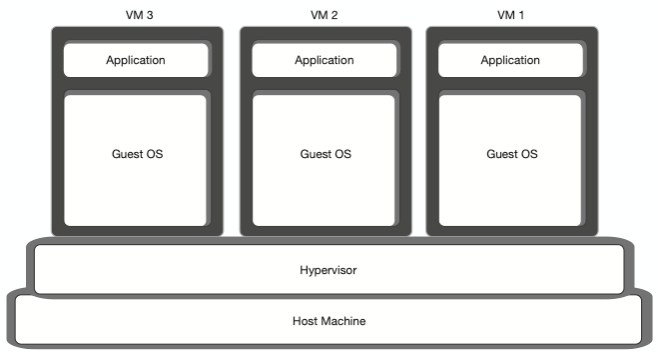
\includegraphics[scale=0.8]{img/full virtualization.png}
    \caption{Full Virtualization}
\end{figure}\noindent

\subsubsection{Para-Virtualization o OS-Assisted Virtualization}
Nella full virtualization i guest OS non devono avere alcuna conoscenza preliminare del fatto che verranno eseguiti su una piattaforma virtualizzata. Questi non hanno bisogno di alcuna modifica speciale (o di incorporare funzionalità) per il funzionamento degli hypervisor e sono installati nel loro “forma” originale. L'intera attività di virtualizzazione è gestita dall'hypervisor, come la traduzione delle istruzioni e l'instaurazione della comunicazione tra diversi sistemi operativi guest e la piattaforma sottostante hardware. \\
Nella para-virtualization viene trasferita una parte dell'attività di gestione della virtualizzazione (dall'hypervisor) verso i guest OS. Le versioni normali dei sistemi operativi disponibili non sono in grado di farlo, hanno quindi bisogno di una modifica speciale per l’aggiunta di questa funzionalità. \\
Questa modifica si chiama \textit{\textbf{porting}}. Viene fatto uno specifico porting per ogni guest OS a seconda del \textit{para-application program interface} (API). Nella figura sottostante è rappresentato un modello di para-virtualization.
\begin{figure}[H]
    \centering
    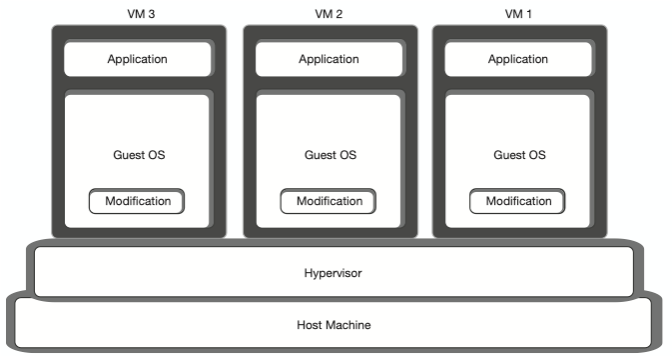
\includegraphics[scale=0.8]{img/Para-virtualization.png}
    \caption{Para-virtualization}
\end{figure}\noindent
In termini di para-virtualization, ogni OS guest deve avere una conoscenza preliminare della piattaforma virtualizzata su cui verrà eseguito. Inoltre, deve anche sapere su quale particolare hypervisor dovrà essere eseguito. A seconda dell'hypervisor, il guest OS viene modificato come richiesto per partecipare all'attività di gestione della virtualizzazione. \\ 
Le versioni non modificate dei sistemi operativi disponibili (come Windows, Linux) non possono essere utilizzate nella para-virtualization. Poiché comporta modifiche del sistema operativo, la para-virtualization viene talvolta definita anche come \textit{\textbf{OS-Assisted Virtualization}}. Questa tecnica allevia in parte l'hypervisor dalla gestione dell'intera attività di virtualizzazione. L'esempio più noto di para-virtualization hypervisor è il progetto Xen open source che utilizza un kernel Linux personalizzato. \\
\textbf{Vantaggi:}
\begin{itemize}
    \item La para-virtualization consente alle chiamate dal guest OS di comunicare direttamente con l'hypervisor (senza alcuna traduzione binaria di istruzioni). L'uso di sistemi operativi modificati riduce il sovraccarico di virtualizzazione dell'hypervisor rispetto alla full virtualization.
    \item Nella para-virtualization il sistema non è limitato dai device drivers forniti dal livello di virtualizzazione software. Di fatto, nella para-virtualization, il livello di virtualizzazione (hypervisor) non contiene alcun device driver. I sistemi operativi guest, invece, contengono i device drivers richiesti.
\end{itemize}
\textbf{Svantaggi:}
\begin{itemize}
    \item Le versioni non modificate dei sistemi operativi disponibili (come Windows o Linux) non sono compatibili con il para-virtualization hypervisor. Gli utenti possono modificare gli open-source OS (come Linux). I sistemi operativi proprietari (come Windows) dipendono dalle decisioni del proprietario. Se il proprietario si impegna a fornire le versioni modificate richieste del sistema operativo per un hypervisor allora solo quel sistema operativo diventa disponibile per il sistema di virtualizzazione. 
    \item La sicurezza è compromessa in questo approccio poiché il guest OS ha un controllo relativamente maggiore dell'hardware sottostante. Quindi, gli utenti di alcune VM con intenzioni malevole hanno più possibilità di causare danni alla macchina fisica.
\end{itemize}
La para-virtualization tuttavia riduce il carico dell’host machine che potrà quindi far girare un numero maggiore di VMs in confronto alla full-virtualization.

\subsubsection{Hardware-Assisted Virtualization}
I fornitori di hardware iniziarono a produrre dispositivi su misura per supportare la virtualizzazione. Intel e AMD hanno iniziato includendo nuove funzionalità di virtualizzazione nei loro processori per andare a ridurre l’overhead dato dalla virtualizzazione e aumentare le performance. L'AMD-Virtualization (AMD-V) e la Intel Virtualization Technology (Intel-VT) consentono ad alcune chiamate privilegiate dalla CPU del guest OS di essere gestite direttamente dalla CPU. Queste chiamate non richiedono di essere tradotte dagli hypervisors eliminando così la necessità della traduzione binaria o para-virtualization. \\
Questo tipo di virtualizzazione è possibile solo quando vengono utilizzate combinazioni specifiche di componenti hardware e ciò è stato possibile solamente dopo il 2006, quando sia Intel che AMD hanno iniziato a includere nuove funzionalità di virtualizzazione nei loro processori. Molti hypervisor bare metal fanno uso di questa tecnologia. Gli hypervisor come Xen, Hyper-V o VMWare ESXi Server di Microsot possono sfruttare i vantaggi della hardware-assisted virtualization. \\
Nella tabella sottostante vengono ricapitolate le differenze tra tre tipi di virtualizzazione:

\begin{table}[H]
    \begin{tabularx}{\linewidth}{X | X | X}
    \hline
    \textbf{Full Virtualization} & \textbf{Para-Virtualization} &
    \textbf{Hardware-Assisted Virtualization}\\ [0.5ex]
    \hline\hline
    Guest OS non ha nessun ruolo nella virtualizzazione &
    Guest OS contribuisce alla virtualizzazione &
    Guest OS non ha nessun ruolo nella virtualizzazione\\
    \hline
    Guest OS non sa di essere virtualizzato &
    Guest OS deve sapere di essere virtualizzato &
    Guest OS non sa di essere virtualizzato \\
    \hline
    Versioni non modificate del OS possono essere usate come guest OS & 
    Sono necessarie modifiche al OS &
    Versioni non modificate del OS possono essere usate come guest OS \\
    \hline
    Fornisce buone opzioni per il guest OS & 
    Fornisce meno opzioni per il guest OS &
    Fornisce buone opzioni per il guest OS \\
    \hline
    Il guest OS non è hypervisor-specific & 
    Il guest OS è progettato specificamente per un hypervisor &
    Il guest OS non è hypervisor-specific \\ 
    \hline
    Non richiede nessuna features speciale alla host CPU &
    Non richiede nessuna features speciale alla host CPU &
    Richiede features speciali alla host CPU \\
    \hline
    L’hardware non gioca alcun ruolo nella virtualizzazione &
    L’hardware non gioca alcun ruolo nella virtualizzazione &
    L’hardware contribuisce alla virtualizzazione \\
    \hline
    L’hypervisor fa carico di tutti i virtualization tasks &
    Guest OS e hypervisor si occupano dei virtualization tasks &
    Un hardware speciale + hypervisor si occupano dei virtualization tasks \\
    \hline
    Il virtualization overhead dell’hyoervisor è maggiore &
    Il virtualization overhead dell’hypervisor è inferiore &
    Il virtualization overhead dell’hyoervisor è inferiore \\
    \hline
    Performance della virtualizzazione sono leggermente lente &
    Performance della virtualizzazione sono migliori &
    Performance della virtualizzazione sono migliori \\
    \hline
    Fornisce un alto livello di sicurezza &
    La sicurezza è compromessa &
    La sicurezza è compromessa dato che le chiamate del guest OS possono accedere direttamente all’hardware \\ [1ex] 
    \end{tabularx}
\end{table}

\subsubsection{Operating System Level Virtualization: Rimozione dell’Hypervisor}
La \textit{operating system level virtualization} (chiamata anche system level virtualization) funziona in modo totalmente diverso rispetto alle tecniche di virtualizzazione descritte precedentemente. Qui il paradigma host-guest non funziona. In questo tipo di tecnica di virtualizzazione, non viene utilizzato alcun hypervisor e i server virtuali sono abilitati dal kernel del sistema operativo della macchina fisica (si può dire che è il kernel stesso l’hypervisor, quindi questo dovrà essere potenziato affinché svolga questo ruolo). L'approccio è mostrato nella figura sottostante.
\begin{figure}[H]
    \centering
    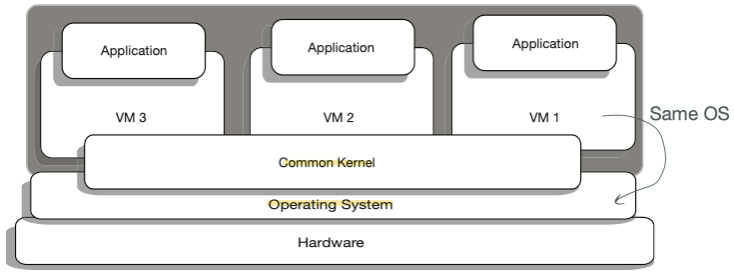
\includegraphics[scale=0.8]{img/operating system level.png}
    \caption{Operating System Level Virtualization}
\end{figure}\noindent
Qui il OS kernel installato sul sistema fisico è condiviso tra tutti i server virtuali su cui sono in esecuzione. Poiché tutti i server virtuali condividono un singolo kernel, è evidente che tutti avranno lo stesso sistema operativo del sistema padre. L'obiettivo di questo approccio è quello di creare più istanze di spazio utente (server virtuali) distinte logicamente su una singola istanza di un OS kernel. \\
\uline{Vantaggi:} È più leggero poiché tutti i server virtuali condividono una singola istanza di un OS kernel. Consente a un singolo sistema fisico di supportare molti più server virtuali rispetto al numero di macchine virtuali complete che potrebbe supportare.
\uline{Svantaggi:} Tutte le macchine virtuali devono usare lo stesso OS (dato che condividono tutte lo stesso kernel). Sono tuttavia consentite diverse distribuzioni (come distribuzioni Linux) dello stesso system kernel. Inoltre, anche la sicurezza è compromessa dato che tutte le macchine virtuali condividono lo stesso kernel.

\subsubsection{Network Virtualization}
La network virtualization è il processo di combinazione di risorse di rete e funzionalità di rete in un'unica entità amministrativa software-based che è chiamata rete virtuale. Questa permette di creare una virtual network per VMs in modo che queste riescano a comunicare tra di loro. La rete virtuale di solito sfrutta la vera infrastruttura della rete per la trasmissione dei dati. Possiamo avere anche più virtual networks sopra alla network fisica, e ognuna di queste sarà isolata dalle altre.

\subsubsection{Storage virtualization}
Nel sistema informatico tradizionale, gli archivi sono sempre stati direttamente collegati ai server fisici. Con la storage virtualization, questo concetto è stato modificato. Ora i sistemi di storage virtualization sono collegati ai server e i sistemi di archiviazione effettivi (fisici) rimangono nascosti. \\
Come altre risorse di elaborazione, anche la storage virtualization avviene tramite un livello software che crea l'astrazione logica del pool di dispositivi fisici di archiviazione collegati tra loro tramite la rete. I dati archiviati nei dispositivi logici (virtualizzati) vengono infine archiviati in alcuni dischi fisici di archiviazione.

\subsubsection{Emulazione}
L'emulazione nell'informatica avviene facendo imitare un sistema ad un altro. Significa che un sistema con una certa architettura è abilitato a supportare il set di istruzioni di qualche altra architettura. Ad esempio, supponiamo che una parte di software sia stata realizzata per l'architettura "A" e non sia supportata dall'architettura "B". Attraverso l'emulazione, è possibile imitare il funzionamento del sistema 'A' (ovvero l'architettura 'A') sul sistema 'B' (cioè l'architettura 'B') e quindi la parte di software può essere eseguita sul sistema B. Gli emulatori possono essere software o hardware. \\ 
Il software di emulazione converte i dati binari scritti per l'esecuzione su una macchina in un modulo binario equivalente adatto per l'esecuzione su un'altra macchina. Questo è fatto traducendo le istruzioni binarie. Ci sono due modi per l'implementazione dell’emulazione, l'interpretazione e la traduzione binaria. 
\begin{itemize}
    \item Nella \textbf{traduzione binaria} (nota anche come ricompilazione), viene eseguita una conversione totale dei dati binari (creata per la piattaforma emulata). La conversione ricompila l'intera istruzione in un'altra forma binaria adatta per essere eseguita sulla piattaforma effettiva o mirata. Ci sono due tipi di traduzione binaria, la ricompilazione statica e la ricompilazione dinamica.
    \item Nell'\textbf{interpretazione}, ogni istruzione viene interpretata dall'emulatore ogni volta che viene rilevata. Il suo metodo è più facile da implementare ma più lento del processo di traduzione binaria.
\end{itemize}

\subsubsection{Emulazione vs Virtualizzazione}
Queste due tecniche sono differenti. \\
La Emulazione permette la simulazione in software dell’intero hardware, creando così l’ambiente per l’esecuzione di un sistema operativo. Può girare sopra l’architettura hardware e può creare l’ambiente per supportare altre architetture oltre a quella dell’host, questo permette a un OS fatto per un determinata architettura di girare in una architettura supportata dall’emulatore. \\
In una semplice virtualizzazione il set di istruzioni usato dal sistema virtuale e l’attuale sistema hardware è lo stesso dato che solitamente l’architettura usata da entrambi sono simili. Quindi la macchina virtuale può semplicemente passare le richieste all’attuale sistema fisico. La traduzione del set di istruzioni non è necessaria. Senza il livello di traduzione (quindi senza la traduzione binaria) le performance della macchina virtuale sono molto più veloci e si avvicinano alla velocità nativa. \\
La virtualizzazione, quindi, è molto più veloce della emulazione. 
\paragraph{Vantaggi della virtualizzazione} 
\begin{itemize}
    \item \uline{Server consolidation:} è il processo che fa girare più macchine virtuali sullo stesso hardware. Questo permette di raggiungere una migliore utilizzazione delle risorse esistenti.
    \item \uline{Riduzione dei costi hardware} e del costo delle infrastrutture informatiche grazie a un migliore utilizzo delle risorse.
    \item Il distacco di hardware e software attraverso un livello di virtualizzazione aiuta a \uline{semplificare l'amministrazione del sistema} impostando due ambienti chiari, uno è l’ambiente guest del sistema operativo e uno è l’ambiente del sistema host.
    \item La virtualizzazione \uline{semplifica l'installazione di un sistema}, in quanto è possibile creare un nuovo sistema clonando un’altra macchina virtuale, senza richiedere l'installazione e la configurazione di un intero sistema.
    \item Migliora la \uline{tolleranza ai guasti} e consente di effettuare la \uline{manutenzione senza dover fermare il servizio} permettendo di migrare le VMs attraverso differenti hardware o di eseguire il backup e ricreare così le VMs.
    \item \uline{Migliora la sicurezza} poiché ogni VM è isolata dalle altre grazie a un ulteriore isolamento fornito dal livello di virtualizzazione 
\end{itemize}
\paragraph{Svantaggi della virtualizzazione}
\begin{itemize}
    \item Ogni macchina fisica è un \textit{\textbf{single point of failure}}. Il principale vantaggio della virtualizzazione è la condivisione delle risorse. Possono essere eseguite più macchine virtuali su una macchina fisica. Ma questo ha un aspetto negativo. Aumenta la probabilità di fallimento di un certo numero di server virtuali nel caso si guasti la singola macchina fisica.
    \item La virtualizzazione si traduce in \uline{prestazioni inferiori}. C'è il dubbio che gli ambienti virtuali siano capaci o meno di emulare le stesse performance del sistema fisico di riferimento. È stato visto che i server virtuali possono raggiungere dall'85\% fino al 90\% delle prestazioni del server fisico effettivo poiché le macchine virtuali non possono accedere direttamente all'hardware.
\end{itemize}

\subsection{Tecniche di Virtualizzazione}
Il processo di virtualizzazione deve garantire alcuni requisiti:
\begin{itemize}
    \item\textbf{Equivalenza}: un sistema operativo in esecuzione in una VM sopra un \textit{hypervisor} (\textit{guest OS}) dovrebbe mostrare un comportamento essenzialmente identico a quello che avrebbe se fosse in esecuzione su un sistema fisico equivalente direttamente.
    \item\textbf{Controllo delle risorse}: l’hypervisor deve avere pieno controllo delle risorse fisiche e, allo stesso modo, il guest OS nella VM deve invece avere un controllo completo sulle risorse virtualizzate.
    \item\textbf{Efficienza}: una frazione statisticamente dominante di istruzioni macchina deve essere eseguita senza l’intervento dell’Hypervisor per garantire efficienza.
\end{itemize}

Tutto ciò deriva dal fatto che il set di istruzioni usato dal sistema virtuale e dall’hardware fisico reale è lo stesso.

\subsubsection{La multiprogrammazione}
I requisiti per la virtualizzazione sono sostanzialmente simili a quanto è richiesto per la multiprogrammazione, attraverso la quale andiamo effettivamente ad emulare la presenza di più processori in una macchina, \textit{\textbf{virtual processors}} o \textit{\textbf{VCPUs}}, rispetto a quanti realmente sono nell’hardware.
Ogni VCPU è riservata all’esecuzione di un processo, il quale deve avere l’impressione di essere l’unico attivo e di avere il pieno controllo del processore, nonostante la componente hardware sia in realtà condivisa.

\paragraph{Esecuzione delle VCPUs}
La multiprogrammazione è possibile grazie al sistema operativo che crea una \textit{rappresentazione virtuale del processore}, nella quale vi è una copia dello \textit{stato del processore reale} (dei suoi registri).
Una macchina con un solo processore fisico emula solo un processore virtuale alla volta, caricando nei registri reali (fisici) del processore host lo stato salvato in quelli virtuali, quindi i valori salvati in una delle rappresentazioni virtuali del processore, e il processore reale continua poi la sua esecuzione a partire dai valori recuperati, finchè non sarà necessario interromperlo per caricare una diversa VCPU.
A questo punto, le strutture dati del processore virtuale saranno aggiornate con i valori attuali contenuti nei registri fisici dell’host, una nuova VCPU verrà selezionata per l’esecuzione e il suo stato sarà prelevato e caricato.
Tutte le CPU virtuali condividono la stessa memoria.

\subparagraph{Cambio di Contesto}
L’operazione di passare da un processo all’altro (e quindi dalle relative VCPUs) viene chiamata \textit{\textbf{cambio di contesto}}.
Essa è determinata dallo \textit{schedulatore} del Sistema Operativo o da un’interruzione (per esempio quando un processo in attesa di un input hardware riceve tale input ed è pronto a continuare la sua esecuzione).
Il cambio di contesto è tipicamente implementato via software dal Sistema Operativo, che si occupa di caricare e prelevare lo stato dei registri del processore in memoria.

\paragraph{Supporto per la Multiprogrammazione}
Nonostante le operazioni precedenti siano gestite dal SO, l’implementazione di un ambiente completo per la multiprogrammazione richiede anche del supporto hardware:
\begin{itemize}
    \item{\textit{Interruzioni} per attivare un cambio di contesto periodico}
    \item{\textit{Meccanismo di protezione della memoria} per isolare le rappresentazioni delle CPU virtuali nella memoria, così da evitare che un dato processo possa accedere alle informazioni dei registri di altri processi (quindi altre VCPUs).}
\end{itemize}
Riguardo al secondo punto, i processori più moderni supportano diversi livelli di privilegi, in particolare, ne includono sempre almeno due:
\begin{itemize}
    \item{\textit{Livello sistema}: ha accesso a tutta la memoria}
    \item{\textit{Livello utente}: ha accesso solo ad una porzione limitata della memoria, che non include le strutture dati delle VCPUs.}
\end{itemize}
Il codice del Sistema Operativo viene sempre eseguito a livello sistema mentre il codice dei processi utente a livello utente.
Ciò significa che quando un processo è in esecuzione il processore lavorerà a livello utente, non potendo quindi accedere alle aree di memoria contenenti informazioni sensibili, relative allo stato delle altre VCPUs. Non appena un’interruzione invoca l’esecuzione di un cambio di contesto, il processore host viene configurato per lavorare a livello sistema, rendendo così possibile l’accesso a quelle aree di memoria necessarie per eseguire l’operazione correttamente.

\subsubsection{Memoria Virtuale}
La memoria virtuale è un meccanismo introdotto per fornire ai processi un’astrazione dalla reale memoria disponibile in un sistema ed usare uno spazio di indirizzamento virtuale.
Quest’ultimo viene creato ed assegnato ad ogni applicazione.
Ciò permette ad ogni processo di pensare di poter accedere ad uno spazio di indirizzi contigui in memoria, a prescindere dalla loro effettiva allocazione fisica in RAM.
I dati in RAM possono essere salvati in segmenti non contigui, in maniera indipendente dagli indirizzi usati dall’applicazione.
Il risultato è che, per via di questa astrazione, ogni processo ha così l’impressione di poter accedere all’intera memoria fisica.
\begin{figure}[H]
    \centering
    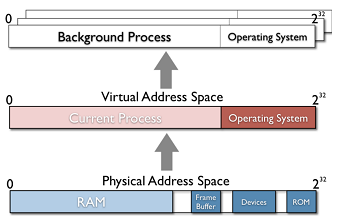
\includegraphics[scale=0.8]{img/Virt_tech/4.png}
    \caption{Indirizzamento}
\end{figure}\noindent

\paragraph{Memory Management Unit}
La memoria virtuale viene implementata attraverso due meccanismi:
\begin{itemize}
    \item\textit{Traduzione degli indirizzi} (da virtuale a fisico): realizzata dalla CPU attraverso uno specifico elemento hardware, la \textit{Memory Management Unit (MMU)}
    \item{\textit{Gestione dello spazio di indirizzamento virtuale} creato per ogni applicazione: realizzata dal Sistema Operativo}
\end{itemize}

\paragraph{Translation Lookaside Buffer (TLB)}
La MMU gestisce la traduzione degli indirizzi in accordo con quanto specificato nel TLB.
La CPU ha un registro, il \textit{Page Table Base Register (PTBR)}, che contiene l’indirizzo fisico del primo byte del TLB. La memoria è organizzata in porzioni di uguale misura (\textit{pagine}).
Il TLB è gestito dal SO ed è organizzato in pagine, ciascuna contenente le informazioni per tradurre una porzione dell’indirizzo virtuale (a partire dai bit più significativi) in indirizzo fisico.
\begin{figure}[H]
    \centering
    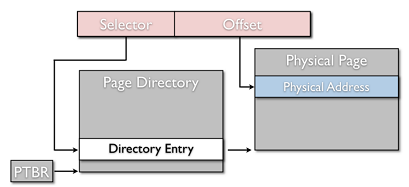
\includegraphics[scale=0.8]{img/Virt_tech/5.png}
    \caption{}
\end{figure}\noindent
Il TLB può essere organizzato in una struttura multi-livello. L’indirizzo virtuale è suddiviso in più parti e sono necessari diversi accessi al TLB per tradurre ciascuna di esse.
La configurazione dipende dall’architettura hardware e dal SO. Per gestire il TLB è necessario supporto hardware.
\begin{figure}[H]
    \centering
    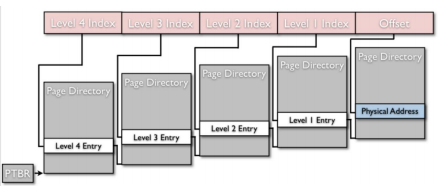
\includegraphics[scale=0.8]{img/Virt_tech/6.png}
    \caption{}
\end{figure}\noindent
\paragraph{Segmentazione}
Lo spazio di indirizzamento virtuale può eccedere la capacità reale della memoria fisica. In questi casi viene sfruttato un elemento secondario per il salvataggio delle informazioni (es. hard disk).
In questo caso, alcune pagine possono essere salvate fuori dalla RAM e quando un programma tenterà di accedervi, non trovandole nella memoria fisica, scatenerà un \textit{page fault}, forzando il SO ad andare a recuperare e spostare tali dati in RAM.
Quando ciò avviene anche il TLB viene aggiornato dal SO.
\begin{figure}[H]
    \centering
    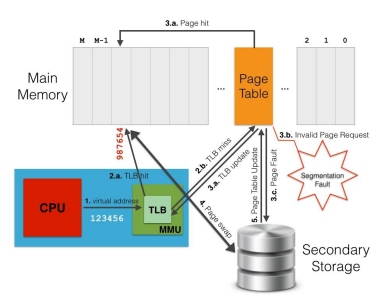
\includegraphics[scale=0.8]{img/Virt_tech/7.png}
    \caption{}
\end{figure}\noindent

\subsubsection{Interruzioni/Eccezioni}
Le interruzioni e le eccezioni vengono usate per notificare al sistema eventi che necessitano di immediata attenzione durante l’esecuzione di un programma.
Esse alterano il normale flusso di istruzioni da eseguire, attivando funzioni specifiche del kernel. L’esecuzione passa dalla modalità utente a quella di sistema, nella quale interruzioni ed eccezioni sono gestite. Al termine l’esecuzione torna nello spazio utente. 
\begin{figure}[H]
    \centering
    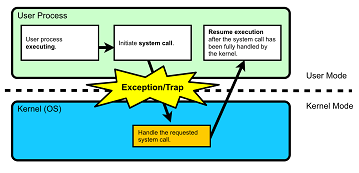
\includegraphics[scale=0.8]{img/Virt_tech/8.png}
    \caption{}
\end{figure}\noindent
Le eccezioni sono interne e sincrone, sono usate per gestire errori interi ai programmi (es. divisione per zero, cattivo indirizzo, page fault).
Un particolare tipo di eccezione è la \textit{trap}, interruzione generata via software, usata anche per le chiamate di sistema.
Le interruzioni sono utilizzate per notificare la CPU di eventi esterni e sono generate dalle componenti hardware esterne al processore, in qualsiasi momento (es. un tasto premuto sulla tastiera).

\subparagraph{Interrupt Descriptor Table (IDT)}
La IDT è una tabella popolata dal SO ed usata dal processore per collegare i vari tipi di interruzioni ed eccezioni ai relativi \textit{handlers}.
Ogni \textit{handler} è una funzione nel kernel che svolge alcune operazioni collegate con una certa interruzione. 
\begin{figure}[H]
    \centering
    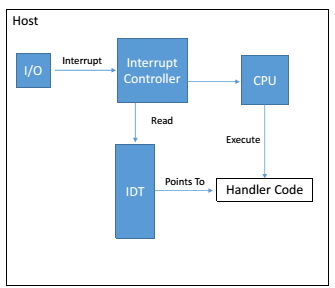
\includegraphics[scale=0.8]{img/Virt_tech/10.png}
    \caption{}
\end{figure}\noindent


\subsubsection{Virtualizzazione tramite Hypervisor}
La multiprogrammazione, come descritto, include già qualche tecnica di virtualizzazione, nello specifico Virtualizzazione a livello Sistema, permettendo così ad ogni processo di avere l’impressione di avere il controllo completo della CPU e della RAM.
Allo stesso modo, anche l’\textit{Hypervisor} (o \textit{Virtual Machine Monitor}) deve dare alle VMs l’impressione di avere pieno controllo dell’hardware fisico (processori, memoria e periferiche di I/O).
Il ruolo dell’\textit{hypervisor} è simile al ruolo svolto dal kernel del sistema operativo. Le sue funzionalità, tuttavia, sono molto più estese, per via della complessità di dover nascondere l'ambiente virtuale alla VM piuttosto che a semplici processi, infatti una VM è di solito un sistema multiprogrammato.

\paragraph{Hypervisor}
L’hypervisor deve essere implementato in maniera tale che emuli un sistema, riutilizzando i meccanismi hardware già disponibili.
Se l’architettura target (da emulare) e quella dell’host sono le stesse, tale risultato può essere raggiunto minimizzando l’utilizzo del meccanismo di emulazione, che introduce un significativo spreco di risorse e rallentamento, per via delle traduzioni binarie necessarie nel passare da un’architettura all’altra in due sistemi diversi.
In questo modo, il codice del SO o di un software in esecuzione su una VM potrà essere eseguito direttamente sull’hardware host, senza bisogno di traduzioni.

\subsubsection{Emulare la CPU}
L’hypervisor gioca un ruolo simile a quello del kernel del SO nella multiprogrammazione, utilizza le stesse tecniche viste per creare le VCPUs:
\begin{itemize}
    \item{Il codice dell’hypervisor è eseguito nello spazio di sistema/kernel (privilegi di sistema) mentre il \textit{guest OS} è eseguito nello spazio utente (privilegi utente).}
    \item{L’hypervisor carica lo stato di una VCPU nel processore host, dopodiché lascia che la host CPU esegua il codice target (guest) così come è, finché la CPU non trova un’istruzione che non possa essere eseguita direttamente ed è richiesto un cambio di contesto.}
    \item{Quando si verifica il cambio di contesto, l’hypervisor riprende il controllo ed emula in software quella istruzione del codice target che non poteva essere eseguita, per poi ricaricare la VCPU precedente nella host CPU, per continuarne l’esecuzione.}
\end{itemize}
Se più VM sono eseguite sullo stesso host fisico, l’hypervisor può schedulare un timer per attivare un cambio di contesto, per assicurare equità tra le differenti VMs che si contendono lo stesso hardware.
In questo caso, allo scadere del timer, l’hypervisor selezionerà un’altra VM per l’esecuzione e lo stato della VCPU sarà caricato sulla host CPU.

Il meccanismo di virtualizzazione però introduce anche aspetti molto differenti da quelli della multiprogrammazione, di cui l’hypervisor deve tenere conto: il guest OS vorrebbe avere il pieno controllo dell’hardware host, vorrebbe quindi poter eseguire anche quelle istruzioni che richiedono privilegi di sistema, non solo utente, e poter accedere ai registri privilegiati.
Per garantire ciò, l’hypervisor deve emulare l’intero processore, non solo a livello utente.
L’hypervisor (VMM) sfrutta le eccezioni/trap per attivare un cambio di contesto dalla VM al VMM ogni volta che viene rilevata un’istruzione che richiede privilegi. 
Il VMM ne fa una traduzione binaria e la esegue, emulandone il comportamento.
Dopo l’esecuzione di quest’ultima, il controllo torna al \textit{guest OS}.
Se il set di istruzioni privilegiate è limitato, tale meccanismo non incide significativamente sulle performance del sistema.
\begin{figure}[H]
    \centering
    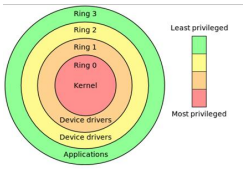
\includegraphics[scale=0.8]{img/Virt_tech/11.png}   
    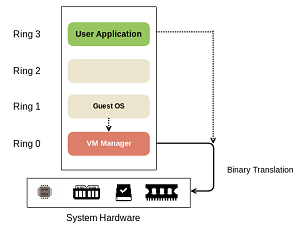
\includegraphics[scale=0.8]{img/Virt_tech/12.png}
    \caption{}
\end{figure}\noindent

\subsubsection{Emulare la Memoria Fisica}
La memoria fisica della \textit{guest VM} è tipicamente implementata usando una porzione della memoria fisica dell’host. Una parte di essa viene riservata per l’esecuzione del VMM mentre la guest VM può avere solo accesso alla porzione ad essa assegnata e deve pensare che la sua memoria inizi dall’indirizzo 0.
Anche in questo caso, per mappare una porzione della memoria fisica della VM con quella dell’host viene utilizzata la MMU della CPU dell’host. Essa è configurata con i range di indirizzi assegnati ad ogni VM e ogni volta che un’istruzione della VM viene eseguita viene effettuata la traduzione degli indirizzi.
Se si verifica un \textit{page fault}, l’hypervisor si occupa di recuperare le pagine mancanti dall’hard disk e caricarle in memoria, per poi configurare la traduzione appropriata nel TLB. 
Alcune operazioni che spetterebbero al guest OS, come aggiornare il TLB, sono quindi gestite dal VMM in realtà.
\begin{figure}[H]
    \centering
    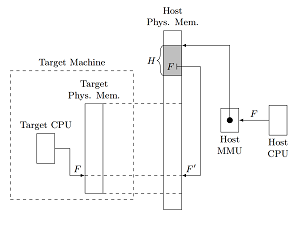
\includegraphics[scale=0.8]{img/Virt_tech/13.png}   
    \caption{}
\end{figure}\noindent

\subsubsection{Emulare dispositivi I/O}
Le istruzioni I/O sono generalmente istruzioni privilegiate, quindi non possono essere eseguite nello spazio utente.
L’hypervisor, al solito, deve dare alla \textit{guest VM} l’illusione di avere il controllo dell’hardware e di potervi accedere direttamente, quindi deve emularlo creandone una rappresentazione virtuale, implementata come un set di strutture dati in memoria.
La guest VM ha accesso a questa rappresentazione virtuale delle periferiche, il VMM vi accede o la modifica ogni volta che una lettura o una scrittura viene eseguita.
Il VMM è l’unico controllore delle periferiche del sistema fisico e può, eventualmente, tradurre un’istruzione I/O destinata ad una periferica virtualizzata in una istruzione I/O per un reale dispositivo I/O, oppure emulare completamente il dispositivo, a seconda della periferica in questione.
\begin{figure}[H]
    \centering
    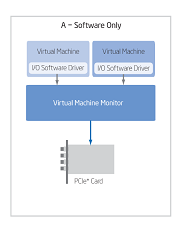
\includegraphics[scale=0.8]{img/Virt_tech/14.png}   
    \caption{}
\end{figure}\noindent

\paragraph{Gestione delle Interruzioni}
L’hypervisor deve occuparsi sia delle interruzioni provenienti dai dispositivi fisici, gestendole in maniera trasparente rispetto alle \textit{guest VMs}, che di quelle generate dai dispositivi virtuali, emulati per il \textit{guest OS}.
A tale scopo, deve mantenere per l’host una tabella di descrizione delle interruzioni (\textit{Interrupt Description Table o IDT}), inaccessibile alle guest VMs, usata dalla host CPU per gestirle. Ogni \textit{guest VM} invece ha la sua IDT gestita dal \textit{guest OS}.
\begin{figure}[H]
    \centering
    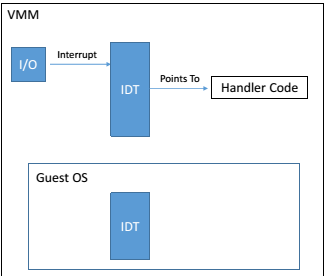
\includegraphics[scale=0.8]{img/Virt_tech/15.png}   
    \caption{}
\end{figure}\noindent

\subsubsection{Emulare le Interruzioni}
Quando l’hypervisor vuole emulare la ricezione di un’interruzione in una VM (per esempio per emulare l’input da un dispositivo virtuale), per prima cosa deve cercare nella \textit{guest IDT} il tipo ricevuto e svolgere le operazioni necessarie per poter eseguire il codice relativo all’\textit{handler} dell’interruzione, cioè:
\begin{itemize}
    \item{Salvare lo stato corrente dei registri nella CPU}
    \item{Cambiare l’\textit{instruction pointer} (il registro nella CPU che contiene l’indirizzo della prossima istruzione da eseguire) con il valore di quello della prima istruzione relativa al codice dell’\textit{handler}}
    \item{Appena l’hypervisor cede nuovamente il controllo alla \textit{guest VM}, essa eseguirà il codice dell’\textit{handler}}
\end{itemize}
L’hypervisor deve considerare che la host CPU potrebbe disabilitare le interruzioni, in quel caso dovrà aspettare finché non verranno nuovamente abilitate, prima di poter emulare la ricezione di un’interruzione.
\begin{figure}[H]
    \centering
    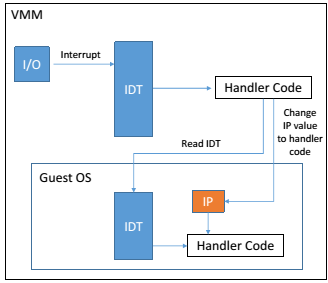
\includegraphics[scale=0.8]{img/Virt_tech/16.png}   
    \caption{}
\end{figure}\noindent

\subsubsection{QEMU}
QEMU (\textit{Quick EMUlator}) è un emulatore open source che fornisce virtualizzazione dell’hardware.
QEMU è un software VMM che emula l’hardware della macchina.
Supporta un vasto set di emulazioni hardware. Può eseguire un \textit{guest OS} con un set di istruzioni differente da quello dell’host, attraverso la traduzione binaria, oppure eseguire una VM con lo stesso set. In quest’ultimo caso QEMU ha un acceleratore per velocizzare l’emulazione.


\subsection{Hardware-Assisted Virtualization}
Le tecniche di Virtualizzazione Hardware consistono nell’eseguire il SO ospite (quello nella macchina virtuale) all’interno dello spazio utente. Ogni volta che il SO ospite utilizza lo spazio kernel, viene eseguito il VMM (Virtual Machine Monitor) – in questo modo le istruzioni privilegiate dell’ospite sono eseguite tramite traduzione binaria. Questa tecnica è utilizzata da VirtualBox.\\
Purtroppo, le operazioni kernel del SO ospite sono molto pensanti dal punto di vista delle prestazioni a causa della traduzione binaria.\\
Pe rimediare a questo problema i processori Intel e AMD sono stati estesi in modo da poter supportare in maniere efficiente l’implementazione di software VMM-Hypervisor. L’estensione Intel si chiama Virtual Machine eXtension (VMX).

\subsubsection{VMX - Virtual Machine eXtension}
La tecnologia VMX introduce due nuovi modi operativi: \textbf{root}, inteso per il VMM che gira sull’host e \textbf{non-root}, inteso per il software ospite in esecuzione dentro la VM. Quindi, si possono avere 4 combinazioni (in ordine di privilegio):
\begin{itemize}
    \item \textbf{root/system}
    \item \textbf{root/user}
    \item \textbf{non-root/system}
    \item \textbf{non-root/user}
\end{itemize}
Le modalità non-root servono per mantenere la distinzione tra codice utente e codice sistema dentro la macchina virtuale.\\
Le modalità \textbf{root} servono all’host. In questo modo il VMM è parte di un SO standard che gira sull’host.\\
Lo scopo principale di queste nuove modalità è quello di inserire delle limitazioni hardware alle azioni svolte dal SO ospite. Quando il SO ospite prova ad eseguire un’istruzione, si troverebbe a violare l’isolamento della VM oppure a richiedere emulazione software.

\paragraph{Esempio} \textit{Il SO ospite deve eseguire una INT o IRET per passare tra le modalità utente e sistema. Senza il supporto hardware, l’esecuzione di queste due istruzioni sarebbe stata emulata via software dal VMM in modo da “mimarne” l’esecuzione (es. modificando i registri manualmente o avviando l’esecuzione di codice kernel).
Con le nuove modalità si può semplicemente passare da \textbf{non-root/user} a \textbf{non-root/system} e viceversa, senza dover emulare l’istruzione.}\\ \\
Le informazioni riguardanti lo stato di una macchina virtuale sono contenuti in una struttura dati chiamata VMCS (Virtual Machine Control Structure), composta dai seguenti campi:
\begin{itemize}
    \item \textbf{Guest State:} Stato del processore (virtuale) associato alla macchina virtuale. Contiene anche l’\textit{instruction pointer} ed il valore da caricare nell’IP alla VM exit.
    \item \textbf{Host State:} Contiene lo stato del processore (fisico) \textbf{prima} dell’avvio della macchina virtuale e viene ripristinato alla VM exit.
    \item \textbf{VM Execution Control:} Specifica quali azioni sono permesse in modalità non-root. Azioni non permesse causano VM exit.
Contiene flag per determinare come gestire interruzioni e operazioni I/O, in particolare se vengono gestite direttamente dalla macchina virtuale oppure se è necessaria una VM exit.
    \item \textbf{VM Exit Control:} Contiene flag che specificano comportamenti opzionali della transizione root/non-root.
    \item \textbf{VM Enter Control:} Inverso dell’Exit Control
    \item \textbf{VM Exit Reason:} Contiene info riguardo al motivo dell’ultima VM exit.
\end{itemize}
\paragraph{MMU Virtuale}
Vogliamo che il SO ospite che gira sulla macchina virtuale abbia la possibilità di fare uso della memoria virtuale. L’ospite avrà la sua funzione di traduzione da indirizzo virtuale a fisico\footnotemark \(G: V \longrightarrow F\) creando e gestendo il proprio TLB.\\
Considerando che la memoria dell’ospite è mappata nella memoria fisica (quella reale dell’host), servirà un ulteriore funzione per tradurre da indirizzo fisico ospite a fisico reale \(H: F \longrightarrow F\)'.
Per implementare questo meccanismo esistono due metodi: \textit{Brute Force} e \textit{Extended Page Tables}.
\footnotetext{: fisico dal punto di vista della macchina virtuale, in realtà non è un vero indirizzo corrispondente ad una cella di memoria.}

\subparagraph{Metodo Brute-Force}
Implementato senza bisogno di alcun supporto hardware da parte dell’host. Il TLB è modificato in modo tale da aggiungervi un nuovo livello (chiamato tabella delle pagine oscure) che dovrà implementare la funzione H.\\
Per far sì che questo nuovo livello funzioni e venga mantenuto aggiornato, la macchina virtuale deve piazzare delle \textit{trap}\footnotemark  su tutte le possibili azioni relative alla MMU e al TLB, in particolare:
\footnotetext{: un tipo di interruzione.}
\begin{itemize}
    \item cambiare un valore al registro PTBR.
    \item cambiare un’entrata al TLB.
\end{itemize}
Ogni volta che una \textit{trap} intercetta un cambiamento nel TLB, il VMM prende il controllo e aggiorna (o aggiunge) una tabella oscura.\\
Questo metodo ha un significativo overhead in quanto richiede numerosi cambi di contesto e continue traduzioni di indirizzi da parte del VMM.

\subparagraph{Metodo Extended Page Tables}
Queste tabelle sono disponibili sull’host ma non sull’hardware emulato per la macchina virtuale. L’hardware che implementa la memoria virtuale dell’host ha due puntatori PTBR: uno al TLB dell’ospite e uno al TLB dell’host. In questo modo è l’hardware ad applicare le funzioni G e H, in sequenza.\\
Grazie a questa estensione non sono più necessarie le VM exit ogni volta che viene modificato il TLB tuttavia, si paga un incremento di costo (computazionale) per la traduzione degli indirizzi che risulta essere più costosa in quanto sono richiesti più accessi in memoria da parte dell’hardware\footnotemark.

\footnotetext{: Per ridurre ulteriormente questo overhead le moderne MMU sono equipaggiate con cache per i TLB.}

\begin{figure}[H]
\centering
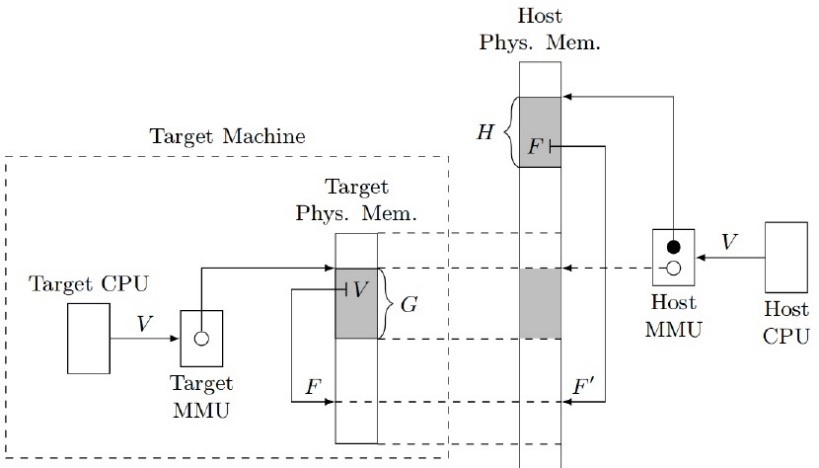
\includegraphics[scale=1]{img/mmu.jpg}
\caption{Mappatura della MMU Virtuale nella Memoria dell'Host}
\end{figure}

\paragraph{Dispositivi di I/O}
L’emulazione dell’I/O è la più grande sfida posta alle macchine virtuali, dal punto di vista delle prestazioni. Il VMM dovrebbe partecipare in ogni interazione tra la macchina virtuale e le periferiche di I/O risultando in numerose VM exit.\\
Per risolvere questo problema diamo, alla macchina virtuale, l’accesso diretto ad una periferica dell’host. Questo approccio si chiama \textit{passthrough} e mappa direttamente il dispositivo nella macchina virtuale senza bisogno di traduzioni, eliminando quindi qualsiasi bisogno di VM exit. Per implementare concretamente questa tecnica serve il supporto esplicito da parte del dispositivo, in particolare:
\begin{itemize}
    \item serve la mappatura diretta dello spazio di I/O (memoria fisica) nella memoria della macchina virtuale, permettendo così al sistema ospite di poter scrivere direttamente nei registri della periferica.
    \item serve l’assegnamento diretto delle interruzioni associate alla periferica in modo tale che la macchina virtuale possa gestire le interruzioni in arrivo dal dispositivo.
\end{itemize}
Per le operazioni di lettura/scrittura da/a registri del dispositivo, vogliamo che l’hardware completi l’operazione senza alcun intervento da parte del VMM. Per tutte le altre operazioni di I/O vogliamo che l’hardware le intercetti come al solito e, dopo, restituisca il controllo al VMM.

\paragraph{Interruzioni}
VMX fornisce due approcci per gestire le interruzioni:
\begin{enumerate}
    \item L’INT causa una VM exit, di conseguenza viene gestita dal VMM.
    \item L’INT viene gestita direttamente dalla macchina virtuale.
\end{enumerate}
Nel secondo caso (utilizzato nell’approccio \textit{passthrough}) l’hardware va a guardare l’entrata corrispondente nella tabella delle interruzioni per eseguire l’handler (del SO ospite) appropriato. Vogliamo anche che la macchina virtuale gestisca le interruzioni in arrivo dal dispositivo \textit{passthrough} anche quando quest’ultima non è in esecuzione.
\begin{itemize}
    \item \textbf{VM in esecuzione:} INT gestita direttamente dal processore.
    \item \textbf{VM pronta:} poiché il processore host sta attualmente eseguendo altro, vogliamo salvare la richiesta di INT in modo tale che la CPU virtuale possa gestirla in un secondo momento (quando andrà in esecuzione).
    \item \textbf{VM ferma:} la INT deve essere salvata e lo stato della macchina virtuale deve essere cambiato a pronto.
\end{itemize}
Per realizzare tutto ciò sono state implementate le \textbf{Interruzioni Posticipate} (posted interrupts) le quali consentono di salvare i segnali di INT per poi notificarli in un secondo momento alla macchina virtuale.
Per ogni macchina virtuale sono necessari dei dati aggiuntivi:
\begin{itemize}
    \item Interrupt Remapping Table (IRT)
    \item Posted Interrupt Descriptor (PID)
\end{itemize}
L’IRT ha un’entrata per ogni possibile INT, ciascuna delle quali mappa la richiesta ad un \textit{vettore di interruzione}\footnotemark  di una CPU o un PID. Quando arriva un segnale di INT la tabella IRT decide se verrà gestita da un vettore di interruzione oppure da un PID (in caso sia abilitato il meccanismo delle interruzioni posticipate).

Lo \textbf{svantaggio} principale dell'\textit{hardware passthrough} è che in caso di molteplici VM in esecuzione su un unico sistema fisico, l'Hypervisor deve garantire l'esclusività periferica passthrough ad una sola VM alla volta.
\footnotetext{: serve per notificare una INT al processore virtuale.}

\paragraph{Virtualizzazione Annidata}
È una tecnica che consiste nell’eseguire l’hypervisor dentro una macchina virtuale che a sua volta è in esecuzione dentro un altro hypervisor.\\
La virtualizzazione annidata è utile principalmente per il testing anche se oggigiorno è utilizzata dai consumatori cloud per costruire infrastrutture IaaS sopra ad un set di macchine virtuali che a loro volta girano su un’infrastruttura IaaS.\\
Intel e AMD supportano solo un livello di virtualizzazione. Per ulteriori livelli è necessario uno specifico supporto hardware.

\newpage
\subsection{Lightweight Virtualization}
\paragraph{Paravirtualization}
La Full Virtualization richiede che sia virtualizzata l'intera architettura, l'hardware virtuale è esposto alla VM dove il OS gira \textbf{immutato}. Le istruzioni del Guest OS che non possono essere eseguite direttamente vengono emulate dalla VMM, quindi senza il supporto hardware l'emulazione viene eseguita ogni volta che si presentano questo tipo di istruzioni portando anche a un overhead significativo.\\
Un approccio alternativo alla Full Virtualization, prima che nascesse il supporto hardware, è la paravitualization. Abbiamo sempre la VMM ma l'hypervisor è implementato partendo dalla assunzione che il \underline{guest OS può essere modificato ed è a conoscenza del fatto di}\\ \underline{star girando all'interno di una VM}. Le modifiche del Guest OS sono limitate solitamente al kernel. Una parte delle funzioni che prima erano implementate dall'hypervisor ora sono state spostate al Guest OS in modo da poter aumentare la performance.\\
Lo scopo è quello di introdurre delle modifiche al Guest OS in modo che si possa impedire al OS di eseguire istruzioni che non possono essere eseguite direttamente (Esempio I/O instructions). Queste istruzioni vengono sostituite con delle chiamate a delle API specifiche esposte dal VMM attraverso una interfaccia chiamata Virtualization Layer. Il VMM è responsabile dell'implementazione di queste funzioni, come creare una rappresentazione virtuale dell'hardware e infine gestire l'hardware reale.\\
Quindi in questa architettura abbiamo ancora un VMM che ha il controllo sul sistema hardware ma espone una interfaccia attraverso la quale il Guest OS potrà interagirci e implementare alcune priviledge instrunctions.\\
\begin{figure}[H]
    \centering
    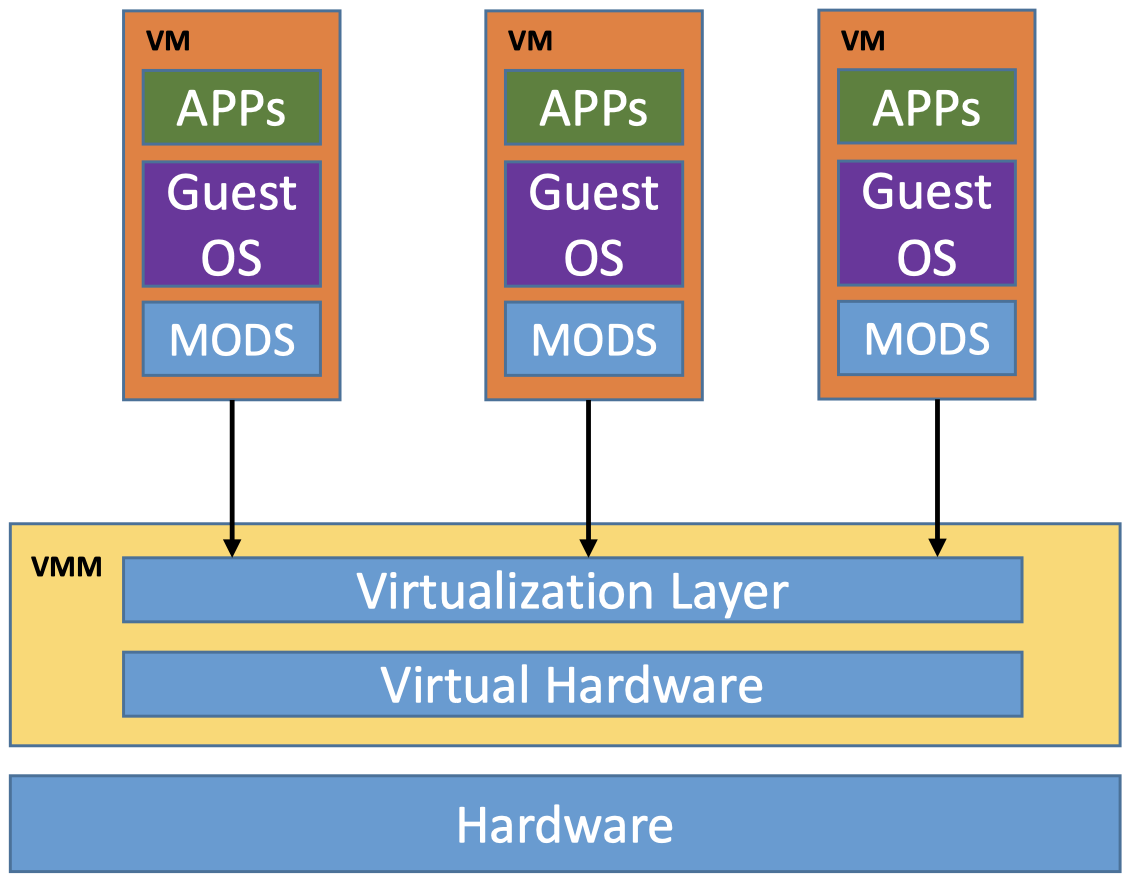
\includegraphics[scale=0.3]{img/Virt_tech/17.png}
    \caption{Paravirtualization Architecture}
\end{figure}
L'emulazione viene evitata andando a modificare il Guest OS e andando a invocare le "Hypercalls", funzioni esposte dal VMM che vanno a sostituire le istruzioni non virtualizzabili. Il codice delle Hypercalls e il VMM vengono eseguiti in system mode, quindi possono andare ad eseguire istruzioni privilegiate e interagire direettamente con l'hardware. Questo permette di ridurre l'overhead dato che non ci saranno i context switch (sono eseguiti in system mode).
\begin{figure}[H]
    \centering
    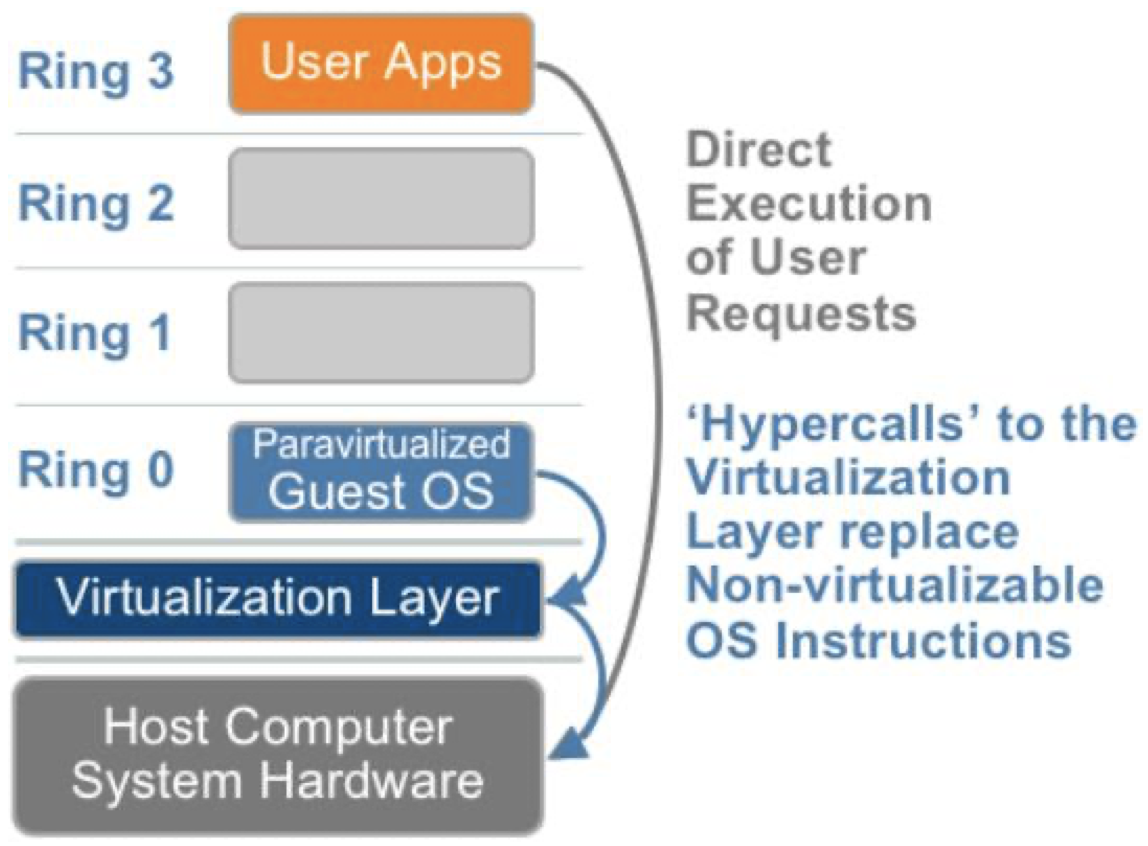
\includegraphics[scale=0.3]{img/Virt_tech/18.png}
    \caption{Paravirtualization Implementation}
\end{figure}\noindent
Pro della Paravitualizzazione:
\begin{itemize}
    \item Non essendoci più uno context switch frequente da OS Guest a Hypervisor (evitando anche l'emulazione) la virtualizzazione ha avuto un significativo aumento nelle perfomance
    \item Non richiede nessun supporto hardware specifico
\end{itemize}
Contro della Paravirtualizzazione:
\begin{itemize}
    \item Supporta solamente delle versioni modificate del OS
    \item Alcuni source OS chiusi non sono supportati
\end{itemize}
Sistemi paravitualizzati, come XEN, erano molto popolari all'inizio per le loro perfomance migliori. Con l'avvento del supporto hardware per la virtualizzazione non era più vantaggioso utilizzare questi sistemi rispetto alla Full Virtualization, quindi non furono più così popolari e furono convertiti in sistemi Full Virtualization.\\ \\
Xen è l'hyoervisor più popolare basato su paravirtualizzazione. Era stato rilasciato nel 2003 prima della nascita del supporto hardware per la virtualizzazione. Era stato creato per ridurre l'overhead della Full Virtualization, dove in sistemi x86 non era semplice andare a virtualizzare usando uno standard trap-and-emulate hypervisor. Xen ha cercato di trovare un compromesso tra lo riscrivere il kernel del OS ed usare troppo la emulazione. È basato su un set di modifiche fatte sul kernel di Linux in modo da poter far girare il OS linux in un modo più efficiente in un modo paravirtualizzato. Dato che il supporto hardware ha reso meno conveniente usare la paravirtulizzazione, Xen ora supporta anche la Full Virtualization con hardware support. In questo modo qualsiasi OS(e non solamente quelli modificati) possono girare su Xen.\\
Xen è un kernel molto piccolo che si è isolato per primo sulla macchina (???) e ottiene il vantaggio di un controllo diretto dell'hardware. Sopra a Xen, con un livello di privilegio più basso, abbiamo i così detti domini. Ci possono essere tanti domini quanti sono necessari, all'interno di ognuno possiamo andare a far girare un intero OS con le sue applicazioni.\\
Un dominio speciale, il Dom0, ha accesso alle API di Xen e può andare a creare o distruggere altri domini. All'interno del Dom0 qualsiasi OS Linux può essere istallato e possono essere sviluppati tools personalizzati che vanno a gestire altri domini. I domini possono avere accesso diretto ad alcuni dispositivi I/O, o possono usare dei dispositivi fully virtualized, o possono usare dei dispositivi paravirtualizzati.
\begin{figure}[H]
    \centering
    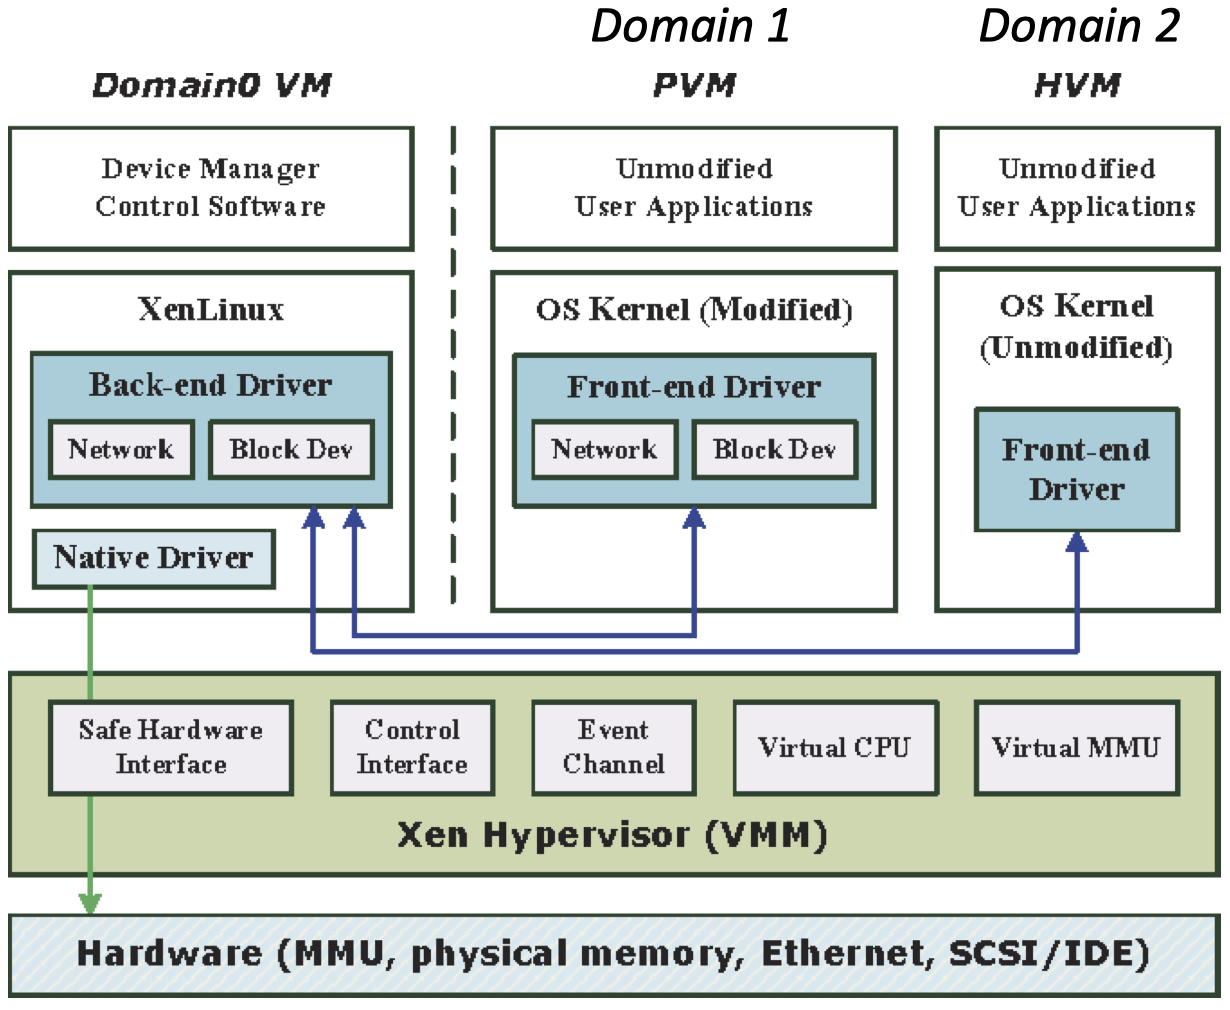
\includegraphics[scale=0.4]{img/Virt_tech/19.png}
    \caption{Xen Hypervisor}
\end{figure}
Uno use-case per la virtualizzazione è poter andare a condividere le risorse hardware tra differenti applicazioni sullo stesso sistema in modo sicuro. L'isolamento delle applicazioni dovrebbe essere fatto dallo stesso OS, comunque, recentemente i OS sono diventati sempre meno efficaci nel garantire l'isolamento. Come conseguenza la configurazione più tipica nel garantire l'isolamento è far girare le applicazioni in differenti VMs. L'overhead portato dalla virtualizzazione non è trascurabile, sia in termini di memoria che di processing time per via del VMM e del guest OS in cui la applicazione gira. Solitamente differenti VMs condividono lo stesso guest OS, come risultato potremmo avere multiple istanze dello stesso OS che girano sullo stesso hardware. (Solitamente in un sistema virtualizzato il guest OS e l'Host OS hanno lo stesso sistema operativo, esempio Linux, e con la virtualizzazione potremmo avere molte full virtualizations tutte con lo stesso OS -> l'overhead è significativo).
\\
La Paravirtualizzazione è ugualmente caratterizzata dall'overhead introdotto dal VMM. In aggiunta, nel caso in cui più istanze dello stesso sistema operativo siano distribuite all'interno delle VM sulle stesse istanze hardware del kernel, i processi del OS e le librerie gireranno sulla macchina. Recentemente sono state introdotte nuove tecnologie di virtualizzazione leggera. Lo scopo è quello di creare un ambiente di esecuzione leggero per i servizi e le applicazioni che non richiedono la virtualizzazione dell'intero sistema ma riescano comunque a garantire gli stessi vantaggi della virtualizzazione ovvero:
\begin{enumerate}
    \item isolamento
    \item dynamic instantiation
    \item ambiente autonomo
\end{enumerate}
Un differente approccio per la virtualizzazione leggera è stato proposto recentemente: \textbf{Operating System Virtualization} o \textbf{Shared Kernel Approaches}. Il suo obiettivo è quello di avere un approccio leggero che vada a minimizzare l'overhead portato dal far girare più VMs con lo stesso OS sullo stesso sistema. Con il OS virtualization l'hypervisor viene rimosso: i server virtuali sono abilitati dal kernel del sistema operativo della macchina fisica. Il kernel del OS è condiviso tra tutti i server virtuali che girano su di esso e dato che questo è condiviso tutte le VMs condivideranno lo stesso OS, che dovrà implementare le istanze dello user space logicamente distinte. Degli esempi sono FreeBSD Jails o Linux Containers.
\begin{figure}[H]
\centering
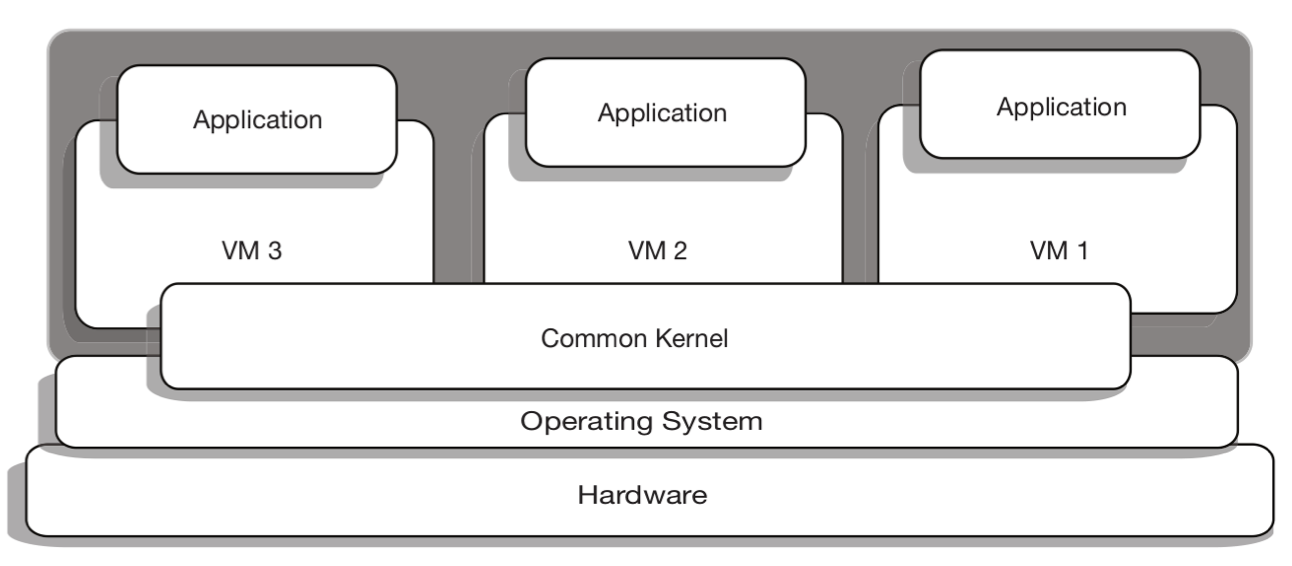
\includegraphics[scale=0.4]{img/Virt_tech/20.png}
\caption{Xen Hypervisor}
\end{figure}\noindent
Pro:
\begin{enumerate}
    \item La virtualizzazione del OS è più leggera per quanto riguarda l'overhead dato che tutti i server virtuali condivideranno la stessa istanza del kernel. Posso avere anche differenti distribuzioni dello stesso OS la cosa importante è che questi abbiano lo stesso kernel.
    \item Un singolo sistema con la stessa quantità di risorse può supportare più VMs rispetto alla full virtualization (non c'è overhead addizionale).
\end{enumerate}
Cons:
\begin{enumerate}
    \item Tutte le VMs devono condividere lo stesso kernel
    \item Non tutti i OSs supportano questo tipo di virtualizzazione (come per la paravirtualizzazione ma solitamente i OSs offrono questo tipo di virtualizzazione)
\end{enumerate}

I containers sono un modo per isolare un set di processi e fargli credere che sono gli unici a girare sulla macchina. La macchina che vedono può avere solo un sottoinsieme delle risorse effettivamente disponibili nell'hardware fisico (esempio meno memoria, meno spazio su disco, meno banda). Quindi in questo contesto il processo ha una visione differente del sistema sotto due punti di vista:
\begin{enumerate}
    \item I processi che possono vedere e quindi con cui possono interagire
    \item il set di risorse disponibili
\end{enumerate}
Per questo i containers non sono full virtualization.
I containers non sono macchine virtuali in generale: i processi che girano al loro interno sono dei normali processi che girano nel kernel dell'host. Di conseguenza non vi è nessun kernel del guest che gira all'interno del container. Per questo motivo non è possibile eseguire un sistema operativo arbitrario in un container. Nel momento in cui il kernel è condiviso con l'host, deve essere lo stesso del host OS. Il vantaggio più grande nell'usare i containers rispetto alle macchine virtuali è la performance: Non vi è alcuna penalità di prestazione nell'eseguire una applicazione all'interno di un container rispetto ad eseguirlo su un host.\\
\begin{figure}[H]
\centering
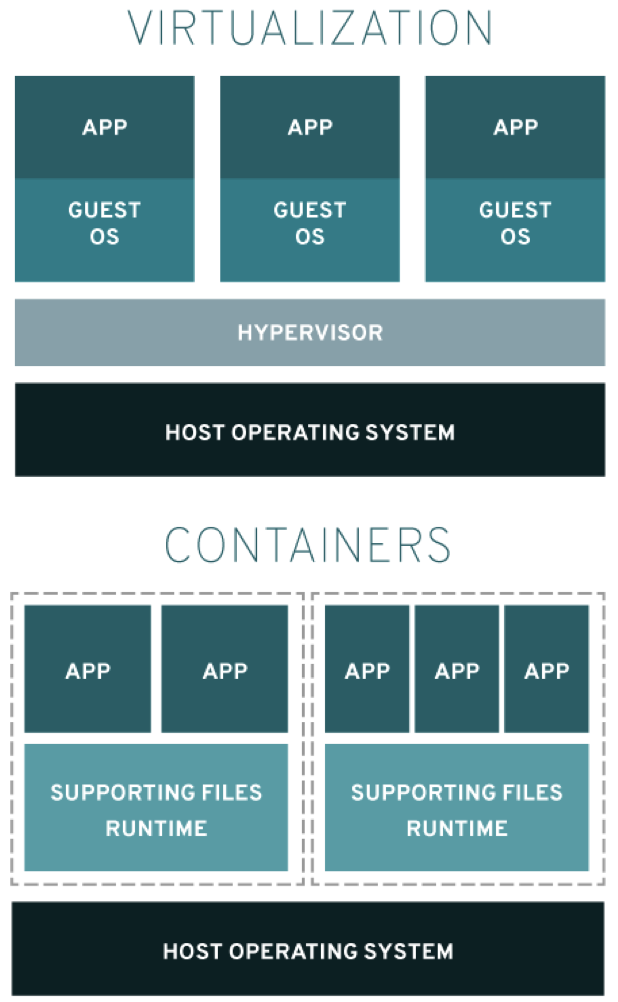
\includegraphics[scale=0.4]{img/Virt_tech/21.png}
\caption{Containers VS Virtualization}
\end{figure}
I containers di Linux sono i più famosi e più utilizzati per virtualizzare il OS. Sono implementati usando due features del kernel: names-spaces e control group. Queste due features si occupano di creare un spazio isolato per far girare l'applicazione che può accedere solamente a un set di risorse (o processi) alle quali è stato dato il permesso di accedere.\\
I Namespaces forniscono un mezzo per separare le risorse di sistema in modo che possano essere nascoste dai processi selezionati. Sono l'estensione di una vecchia funzione Unix: chroot(), una system call che permette a un processo di specificare una porzione del file system al quale l'applicazione è confinata. Usando chroot un utente root seleziona una subdirectory (un sotto albero dele file system) che sarà la radice del file system del processo. È stato definito per confinare il processo non attendibile ad una parte del file system in modo che possano accedere solo ai file di cui hanno bisogno, quindi andando ad aumentare la sicurezza del sistema e successivamente fu esteso al namespace. 
\begin{figure}[H]
\centering
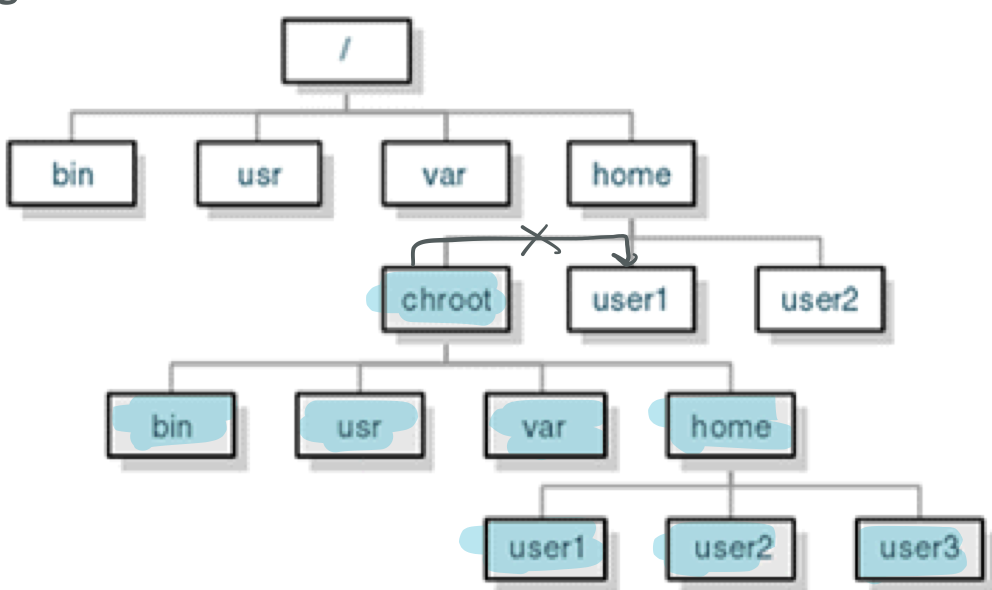
\includegraphics[scale=0.5]{img/Virt_tech/22.png}
\caption{Containers VS Virtualization}
\end{figure}
Quest'ultimo fu introdotto per nascondere o creare altre copie di altre risorse di sistema. Differenti namespaces sono definiti, esempio sono i network namespaces che servono per nascondere le network interfaces o per creare delle interfaccie virtuali, pid namespaces che servono per nascondere i processi.
\\ \\
I namespaces non sono sufficienti per isolare un insieme di processi in modo che questi non interferiscono con gli altri. Anche se il processo non può interagire con gli altri, questi possono abusare delle risorse di sistema ad esempio allocando troppa memoria, usando la CPU per troppo tempo o andando usare troppa banda. \textbf{I control groups sono dei gruppi di processi, per i quali l'utilizzo delle risorse è controllato e forzato}. Questi sono creati dall'amministratore di sistema (root user), ogni processo deve appartenere a un gruppo dal quale non può fuggire. Quando un processo crea un processo figlio (utilizzando la fork() ad esempio) questo andrà ad ereditare il control group del padre. Ogni gruppo può essere collegato a uno o più sottosistemi per andare a limitare l'accesso alle risorse di sistema, come ad esempio: memoria, per limitare la quantità di RAM accessibile ad ogni gruppo; cpu, per limitare la massima frazione di CPU che ogni gruppo può usare.
\\ \\
Il namespace e il control group gestiscono anche l'hardisk nei containers o sono condivisi dal guest OS?\\
Con i containers non abbiamo un guest OS, noi abbiamo un ambiente che supporta l'esecuzione della applicazione. Le periferiche, eventualmente, sono gestite dal OS dell'host e dal kernel dell'host che è condiviso dai differenti containers. Il software che gira all'interno del container non ha accesso all'hard drive ma al file system, che potrebbe essere solamente un sottoinsieme e non tutto il file system del OS dell'host. Quindi il namespace crea un file sistem customizzato e quindi in termini di file system possiamo dire che il container vede solamente un sottoinsieme del file system. Altre periferiche potrebbero avere solamente una rappresentazione virtualizzata, ad esempio il container potrrebbe avere accesso a una interfaccia della network virtualizzata che potrebbe essere connessa fisicamente all'interfaccia reale della network. Quindi ogni container potrebbe avere una netwrok virtuale che è gestita dal kernel dell'host e che si occupa di andare a gestire il traffico e inoltrarlo ad internet se il container ha il peermesso di farlo.
\\ \\
Oltre che provvedere una virtualizzazione leggera i containers sono utilizzati per il software distribution. Un esempio è \textbf{Docker}, un sistema popolare che sfrutta la virtualizzazione a livello di sistema operativo per distribuire pacchetti software in container che hanno al loro interno tutto quello che è necessario per l'esecuzione del software. Questi infatti provvedono un bundle isolato in cui il software, le librerie e i file di configurazione possono essere inclusi. Un package Docker dopo l'installazione è pronto per essere eseguito, non richiede l'installazione di librerie addizionali o dipendenze grazie al fatto che i containers non cambiano da una macchina all'altra. \\
L'architettura di Docker permette di instanziare i containers sul sisteema basandosi su una immagine scaricata da una repository centralizzata, la Docker registry. Un host eseguirà la Docker engine che può essere scaricata e andrà a eseguire un container scaricato dal registry. I Software bundles possono essere caricato dagli sviluppatori sul registry, mentre la Docker engine locale provvede a fornire una interfaccia all'utente per poter andaree a selezionare e installare i package del software.
\begin{figure}[H]
\centering
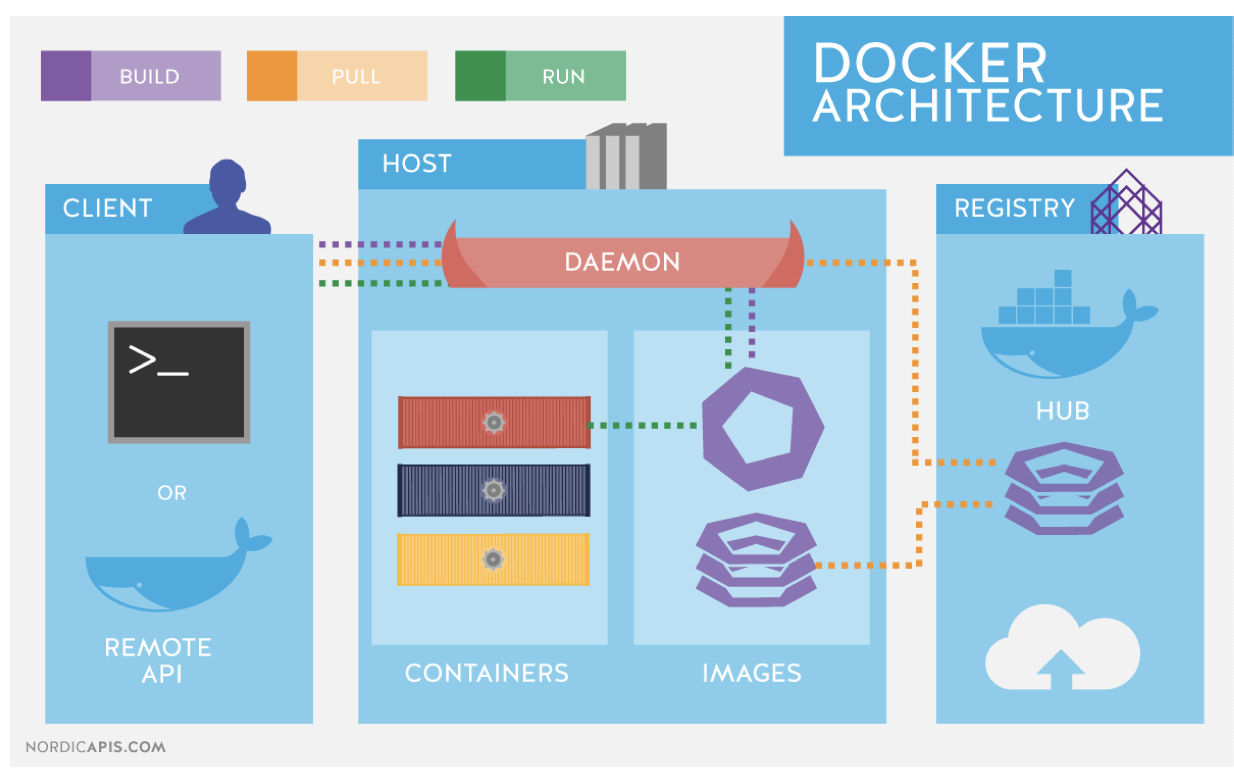
\includegraphics[scale=0.5]{img/Virt_tech/23.png}
\caption{Containers VS Virtualization}
\end{figure}
I containers hanno avviato un nuovo modello di cloud computing: Serveless computing o microservices. I consumers del Cloud non andranno a creare delle full VMs per andare a implementare i loro servizi (o software) sul cloud, ma andranno a creare e implementare dei containers con il loro software che gira all'interno di un ambiente da loro preparato in maniera tale che sia subito pronto all'uso (invece che andare a provvedere una macchina full virtualized). I Cloud providers vendono i servizi basandosi su questo modello, nuove piattaforme cloud sono state create per supportare questo (lo vedremo poi nel dettaglio).

\newpage
\section{Applicazioni Cloud}
Per quanto visto finora, il cloud è un’infrastruttura che offre la possibilità di creare VMs. Ognuna di esse ha una o più Virtual CPUs, la propria RAM e un hard-drive locale, sul quale è installato il \textit{guest OS}, eseguito sulla VM. 
Le VMs hanno anche un adattatore di rete virtuale attraverso il quale esse possono comunicare con altre VMs, tramite LAN virtuale o fisica, o con \textit{hosts} esterni, via Internet.
Le VMs possono avere accesso ad un \textit{cloud storage}, cioè ad uno spazio di archiviazione, fisico o virtualizzato, condiviso tra tutte le VMs, solitamente accessibile tramite la LAN che connette le VMs.

\paragraph{Applicazioni tradizionali}
Le applicazioni progettate e implementate seguendo il modello computazionale tradizionale hanno una struttura molto semplice: da un lato abbiamo un \textit{application server} centrale (server fisico) su cui viene eseguito il servizio che implementa la logica dell’applicazione e nel suo hard disk locale vengono salvati tutti i dati, dall’altro un insieme di \textit{clients} (\textit{browser web} o applicazioni \textit{mobile/desktop}) che forniscono all’utente un’interfaccia per accedere al sistema. Clients e application server comunicano generalmente usando la rete (LAN o WAN). \\ \\Il primo passo per passare ad applicazioni cloud è quello di trasferire l’intera implementazione dell’application server già esistente, servizi e dati, dall’hardware fisico alle VMs nel cloud.
L’architettura dell’intero sistema rimarrà la stessa, da un lato rimane l’application server, ora installato sul cloud, e dall’altra i clients che interagiscono con il precedente sempre tramite la rete.
Trasferire semplicemente un servizio già esistente sul cloud, mantenendone però l’architettura tradizionale, permette di avere alcuni benefici, come la riduzione dei costi, ma non sfrutta a pieno le potenzialità di tale sistema.

\subsection{Architetture Cloud}
Le applicazioni cloud sono generalmente implementate come sistemi multilivello, in cui differenti VMs eseguono differenti funzionalità e possono essere distribuite diverse alternative, a seconda dei requisiti e casi d’uso dell’applicazione. 
L’architettura più semplice consiste in due livelli, il primo, l’application server, in cui vengono gestite le richieste dei clients, e un secondo livello per la gestione dati (\textit{Database Tier}), con il quale interagisce il precedente per recuperare o salvare dati come specificato nelle richieste, così da separare le due funzionalità. \\Può essere aggiunto un ulteriore livello che si occupi esclusivamente dell’archiviazione dei dati (\textit{Storage Tier}), che fornisce uno spazio di archiviazione condiviso accessibile da diverse VMs.
Quando il livello applicazione riceve una richiesta e necessita di recupare un dato, inoltra la richiesta ad una delle VM nel livello database che a sua volta interagisce con il livello di archiviazione per il recupero del dato.
\begin{figure}[H]
\centering
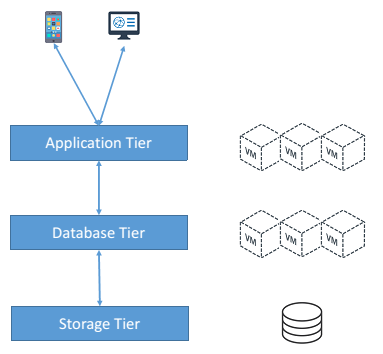
\includegraphics[scale=0.6]{img/base_arch.png}
\caption{Architettura base per Applicazioni Cloud}
\end{figure}

Il risultato in generale sarà un’architettura multilivello in cui il servizio viene fornito al client attraverso una \textit{catena di interazioni} (client/server) tra i server dei diversi livelli che sono connessi tramite LAN e usano un protocollo applicazione che può essere implementato da un software di middleware.
\begin{figure}[H]
\centering
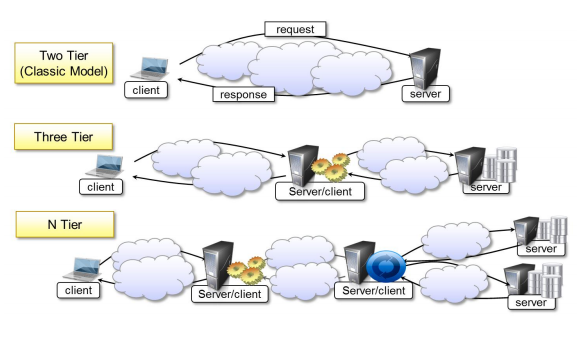
\includegraphics[scale=0.6]{img/interaction_chain.png}
\caption{Interazione tra i livelli}
\end{figure}
\paragraph{Compute Cluster}
Il set delle VMs appartenenti ai differenti livelli che implementano un’applicazione viene detto \textit{compute cluster} ed è organizzato in maniera tale da eseguire delle operazioni collettive relative ad un singolo grande lavoro. La struttura globale del cluster può essere molto diversa a seconda dei requisiti specifici dell’applicazione e dei casi d’uso.
I nodi non eseguono molte operazioni di I/O se non quelle necessarie per trasferire i dati tra i nodi del cluster.
Essi comunicano tra loro (tra VMs dello stesso livello o di diversi livelli) usando un software di middleware.

\subsubsection{High-Availability Clusters}
Essi sono cluster progettati per essere tolleranti ai guasti e supportano l’esecuzione di quei servizi che richiedono di essere sempre (o per la maggior parte del tempo) disponibili. 
Vengono utilizzati dei nodi ridondanti così da evitare i \textit{single-point-of-failure}.
Maggiore è la ridondanza, più elevata sarà la disponibilità, per questo in ogni livello dovrebbero esserci diversi nodi in grado di eseguire le stesse operazioni o fornire lo stesso servizio.

\paragraph{Architettura negli HA Clusters} L’architettura utilizzata è di tipo \textit{master/slave}: tra i nodi ridondanti di un livello viene selezionato un master e tutti gli altri saranno settati come \textit{slaves}.
Il master svolge la funzionalità assegnata ad un certo livello mentre gli slaves fungono da backup. In caso di fallimento del master ne viene selezionato momentaneamente un altro tra gli slaves tramite procedura di elezione o ordine statico.
Affinchè le funzionalità di master vengano svolte correttamente anche dal nuovo nodo eletto è necessario includere anche un meccanismo di replica per replicare dati, configurazioni e altre impostazioni anche sugli slaves.
\begin{figure}[H]
\centering
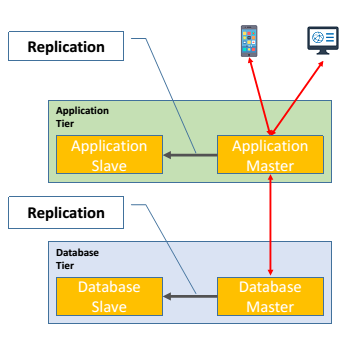
\includegraphics[scale=0.6]{img/HACluster_Arch.png}
\caption{Architettura di un High-Availability Cluster}
\end{figure}

\subsubsection{Load-Balancing Cluster}
Permettono di migliore l’utilizzo di tutte le risorse disponibili sul cluster, bilanciando il carico delle richieste in arrivo tra tutti i nodi partecipanti. Ciò permette di assicurare la scalabilità, in quanto tutti i nodi si dividono il carico di lavoro, e di migliore le prestazioni, come la riduzione dei tempi di risposta.

\paragraph{Architettura negli LB Clusters} Il bilanciamento del carico è ottenuto introducendo un ulteriore livello tra quello dell’applicazione e quello dei clients (\textit{Balancer Tier}), formato da diverse VMs. I client inviano le richieste ad una di esse che a loro volta le inoltreranno verso una delle VM del livello applicazione, seguendo un certo criterio, per esempio verso quella che attualmente ha meno richieste da servire. La VM del livello applicazione inoltrerà poi la richiesta ad un certo nodo, assegnato, del livello database, così da avere un carico nell’insieme bilanciato.

\begin{figure}[H]
\centering
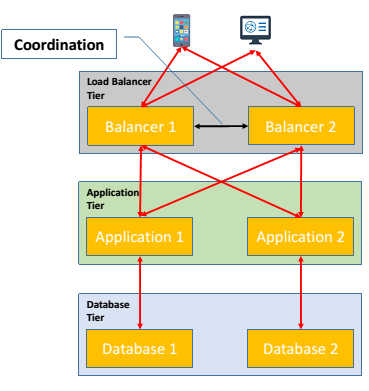
\includegraphics[scale=0.6]{img/LBCluster_Arch.png}
\caption{Architettura di un Load-Balancing Cluster}
\end{figure}

\paragraph{Sincronizzazione dei Dati}
I dati dello stesso livello devono essere coerenti (sincronizzati) tra loro. Un modo per ottenere ciò, evitando l’\textit{overhead} generato invece dalla replica dei dati, è quello di usare un livello di archiviazione condiviso (spostando così la complessità della gestione dei dati condivisi su questo livello). 
La scelta del metodo da usare dipende dai casi d’uso e dalla quantità di dati da salvare: la replica dei dati tra i nodi dello stesso livello è una soluzione nei casi in cui le informazioni da salvare (e quindi replicare) non siano elevate.
\begin{figure}[H]
\centering
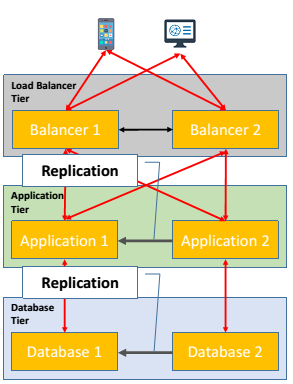
\includegraphics[scale=0.6]{img/DataSync_Replica.png}
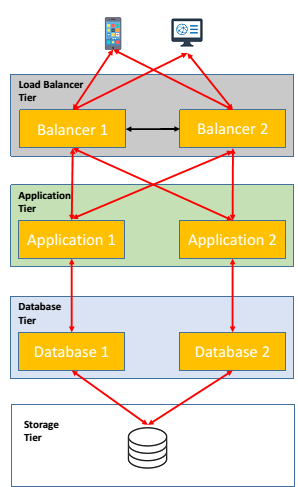
\includegraphics[scale=0.6]{img/DataSync_SharedStorage.png}
\caption{Replica dei Dati vs Archiviazione Condivisa}
\end{figure}

\subsubsection{Compute Intensive Cluster}
Cluster progettato per analizzare una grande quantità di dati (es. big data analytics). 
Adotta un approccio \textit{“divide et impera”}:
\begin{itemize}
    \item Il task di analisi viene suddiviso in sub-tasks (\textit{\textbf{Jobs}}).
    \item I dati sono suddivisi in blocchi più piccoli, detti \textit{\textbf{chunk}}, ognuno dei quali viene assegnato ad un \textit{\textbf{job}}.
    \item Un \textit{job} (ed il relativo \textit{chunk}) viene poi assegnato ad un server (\textit{\textbf{worker}}) per l’analisi.
    \item Il server esegue le operazioni di analisi sui dati assegnati a restituisce i risultati ad un \textit{\textbf{collector}}.
    \item Il \textit{collector} rimette insieme tutti i risultati.
\end{itemize}
Un esempio di applicazione di questo approccio si ha negli algoritmi di ricerca nel web: i dati del web sono tantissimi per essere gestiti da una sola macchina, perciò i dati da analizzare, per la ricerca di determinate parole chiave, vengono suddivisi in \textit{chunk} e assegnati a differenti \textit{workers}, un \textit{collector} riceve tutti i risultati da questi ultimi e li aggrega.
\paragraph{Architettura in un CI Cluster}
Per garantire la scalabilità con un elevato numero di richieste è necessario prima di tutto introdurre un livello \textit{load balancer} (obbligatorio in applicazioni pubbliche come un motore di ricerca). Dopodichè, ogni istanza nel livello applicazione divide i dati in \textit{chunk} e crea una lista di \textit{jobs}. Il dataset iniziale è contenuto nello spazio di archiviazione condiviso (\textit{storage tier}) in quanto è impossibile salvare in locale in ogni nodo tutti i dati e garantirne la coerenza (sincronizzazione), per via della dimensione dei dati. I Job sono distribuiti poi tra i vari workers che appartengono ad una infrastruttura distribuita di elaborazione (insieme di VMs), la quale può avere accesso diretto allo Storage Tier, così i nodi del livello applicazione non dovranno inviare interamente i dati ma solo dei puntatori, con i quali i workers potranno poi accedere direttamente alla porzione di informazioni ad essi assegnata nello storage tier, evitando così un overhead nello scambio di dati tra un livello e l'altro.

\begin{figure}[H]
\centering
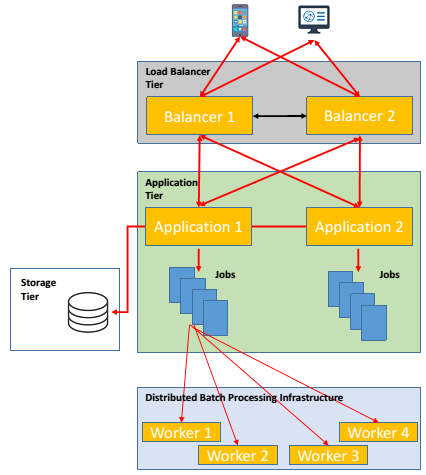
\includegraphics[scale=0.6]{img/CICluster_Arch.png}
\caption{Architettura in un Compute Intesive Cluster}
\end{figure}

\paragraph{Adattamento Dinamico}
Uno dei maggiori vantaggi delle tecnologie cloud, come abbiamo visto, è la possibilità di scalare facilmente quando il carico di lavoro aumenta, sfruttando la scalabilità orizzontale (aumentando il numero di VMs disponibili per processare le richieste).
Le architetture LB e CI, che contengono un livello di bilanciamento del carico iniziale, si prestano molto bene ad adeguarsi alle continue variazioni dell’ammontare di richieste in arrivo: quando il traffico aumenta nuove VMs vengono create e aggiunte a tale livello, così da ridurre il carico di lavoro su ciascuna di esse. Al contrario, se il traffico diminuisce, le VMs possono essere deallocate, così le risorse non sono sprecate.
Nell’architettura HA, invece, la scalabilità orizzontale può essere sfruttata per incrementare la ridondanza dei nodi (più macchine virtuali significa più disponibilità) o per ribilanciare il livello in caso d fallimenti.

\subsection{Design di Applicazioni Cloud}
Le applicazioni cloud sono sistemi distribuiti: con l’aumentare della loro complessità tutta la logica, funzionalità e dati ad esse collegati vengono distribuiti su differenti sistemi (in questo caso Macchine Virtuali), che includono diversi componenti software capaci di interagire tra loro per fornire un servizio (applicazione) agli utenti. \\Tali sistemi distribuiti sono generalmente \textit{sistemi eterogenei} in cui diversi tipi di risorse (es. diversi processori, ecc) sono integrate per formare un unico sistema. \\Nasce quindi l’esigenza di garantire alle applicazioni \textit{interoperabilità} con l’ambiente disponibile. \\ \\L’implementazione e integrazione di differenti componenti software per l’ambiente cloud è un’operazione complessa che può richiedere molto tempo ed essere costosa, rallentando così anche i tempi di messa in commercio di determinati software. \\Per evitare ciò è necessario utilizzare un approccio comune e rigoroso, nel progettare e sviluppare oggetti software, soprattutto in un ambiente dinamico come il cloud.\\ \\Un software, parte di un’applicazione cloud, dovrebbe essere progettato rispettando i seguenti requisiti:
\begin{itemize}
    \item \textbf{Interoperabilità e integrazione}: diversi componenti software possono interagire tra loro e affinché ciò sia possibile occorre che il software esponga un’interfaccia standard, facilmente raggiungibile dagli altri software/componenti dell’applicazione
	\item \textbf{Scalabilità}:  una delle caratteristiche fondamentali dell’infrastruttura cloud è la possibilità di scalare orizzontalmente con l’aumentare degli utenti, perciò l’applicazione deve essere progettata in maniera tale da poter integrare dinamicamente e facilmente un crescente numero di componenti 
    \item \textbf{Componibilità}:  l’ambiente su cui si sviluppa il cloud può cambiare rapidamente per via di fallimenti dei componenti, creazione/distruzione delle VM, ecc. Un software non deve dipendere dalla struttura di tale ambiente. Deve essere progettato in modo da non risentire di possibili cambiamenti e continuare a funzionare con componenti differenti senza bisogno di modifiche (o minime).
\end{itemize}

\subsection{Architettura Service-Oriented}
Negli ultimi anni, tra i vari modelli di sviluppo per le applicazioni cloud, è emerso un approccio architetturale \textit{orientato ai servizi}, la cosiddetta \textbf{\textit{Service-Oriented Architecture (SOA)}}, che supporta l’interoperabilità dei componenti software, insieme alla modularità e alla loro riusabilità, facilitando la scalabilità orizzontale nelle applicazioni.
L’architettura orientata ai servizi viene incontro a quelli che sono i principali obiettivi del cloud computing, quali l’ottenimento di un sistema più flessibile, di facile mantenimento e a costi ridotti, in un ambiente estremamente dinamico.\\ \\In questo tipo di modello, ogni componente software è considerato come un \textbf{servizio} a sé stante che implementa funzionalità specifiche.
Le applicazioni in SOA sono realizzate come \textit{collezioni di servizi}, attraverso componenti software esistenti, in maniera modulare.
I servizi software possono essere sviluppati usando diversi linguaggi di programmazione ed essere eseguiti su diverse piattaforme, in maniera distribuita. Un’applicazione può sfruttare uno o più di tali servizi e SOA permette di integrare i diversi componenti attraverso un approccio indipendente da linguaggio e piattaforma utilizzati.
I \textit{servizi Web} sono un esempio del più comune utilizzo di implementazioni SOA.
\subsubsection{Architettura}
I servizi all’interno di un’applicazione comunicano via \textbf{\textit{message passing}}. 
Ogni messaggio ha uno schema specifico per definire il formato dell’informazione che deve fornire un servizio e come deve avvenirne lo scambio.
I messaggi sono inviati tra i servizi e ognuno di essi li gestisce diversamente al suo interno.

\begin{figure}[H]
\centering
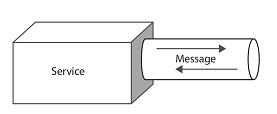
\includegraphics{img/message_passing.png}
\caption{Schema Message Passing}
\end{figure}

\paragraph{Ruoli}
In un’interazione in SOA possiamo distinguere due  ruoli:
\begin{itemize}
    \item \textbf{\textit{Consumer Service}}:  invia una richiesta per ricevere un certo servizio tramite message passing
	\item \textbf{\textit{Provider Service}}:  fornisce al consumatore i risultati richiesti
\end{itemize}
Lo stesso servizio può implementare entrambi i ruoli, a seconda della situazione. \\In genere provider e consumatore non dialogano direttamente, dato che il consumatore dovrebbe conoscere a priori l'indirizzo ed il descrittore del provider. Qui entra in gioco un terzo ruolo molto importante, che fa da intermediario tra i due ruoli precedenti:
\begin{itemize}
    \item \textbf{\textit{Broker}}: crea una sorta di catalogo su cui sono presenti tutti servizi disponibili (\textit{service catalog}).  \\ Il broker sa quando viene creata un'istanza di un certo provider service perciò ogni volta che un consumatore richiede quel servizio, il broker può assegnare un'istanza di esso tra quelle presenti. Se diversi consumatori richiedono lo stesso servizio, ad ognuno di essere sarà assegnata una diversa istanza di esso.
    Il broker conosce sempre tutte le istanze disponibili. Se una di esse viene distrutta, è l'istanza stessa che nel suo distruttore manderà un avviso al broker (non è il sistema che lo notifica).
\end{itemize}
L'indirizzo e il descrittore del broker sono noti perciò un consumatore può fin da subito interagire con esso. Un servizio client potrà usufruire di un servizio solo se la relativa interfaccia è presente nel broker. Una volta interrogato il broker per uno specifico provider service e ottenuta la sua identità, il client potrà contattarlo ed interagire direttamente con esso.
\begin{figure}[H]
\centering
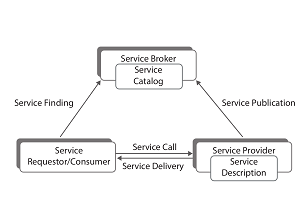
\includegraphics{img/broker_Arch.png}
\caption{Architettura in SOA}
\end{figure}

\paragraph{Vantaggi}
L'implementazione dei servizi rimane nascosta, dando così la possibilità di risolvere eventuali problemi di implementazione del singolo senza interessare gli altri, almeno fin quando la sua dichiarazione/interfaccia rimane intatta. \\ 
I vantaggi che ne derivano sono:
\begin{itemize}
    \item \textit{\textbf{loose coupling} ("Accoppiamento allentato"}: consente di collegare e scollegare i servizi specifici da un'applicazione senza sforzo. Questa caratteristica rende il sistema flessibile nei cambiamenti ed espandibile, nuove funzionalità possono essere aggiunte in breve tempo.
    \item \textit{\textbf{Componibilità}}: un sistema può essere ottenuto dall'unione di più servizi già esistenti.
    \item \textit{\textbf{Comunicazione senza stato}}: la comunicazione è basata sullo scambio di messaggi, un modolo tratta ogni transazione separatamente, in maniera indipendente dalle altre.
    \item \textit{\textbf{Scalabilità}}: le caratteristiche precedenti rendono i servizi SOA particolarmente adatti alla scalabilità dell'infrastruttura del cloud. Il broker gioca un ruolo fondamentale nella gestione dinamica dei servizi che vengono continuamente creati/distrutti per assecondare le richieste dei consumatori. Quando una nuova istanza di un servizio viene creata essa viene registrata dal broker e resa disponibile al consumatore per poi essere deregistrata quando viene distrutta, tutto in maniera trasparente al consumatore.
\end{itemize}

\subsubsection{Servizi Web}
I servizi web sono la naturale evoluzione e adozione del paradigma SOA nel Web. Essi hanno un'interfaccia descritta in un formato eseguibile da una macchina, il \textbf{Web Services Description Language (WSDL)}, usato per interagire con il \textit{broker}. Tramite WSDL ogni \textit{service provider} si registra al \textit{service broker} mentre il \textit{service consumer} utilizza WSDL per cercare uno specifico servizio.
Consumer e provider interagiscono tra loro usando il \textbf{Simple Object Access Protocol (SOAP)}.
\begin{figure}[H]
\centering
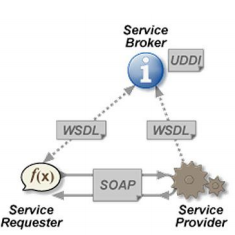
\includegraphics{img/wsdl.png}
\caption{Interazioni nei Servizi Web}
\end{figure}

\paragraph{SOAP}
Fornisce una struttura standard di \textit{packaging} per la trasmissione di documenti XML su vari protocolli internet. Un messaggio in SOAP è formato da un elemento \textit{root} chiamato \textbf{SOAP envelope}, che ha al suo interno un \textbf{header} ed un \textbf{body}. L'header contiene alcune informazioni aggiuntive, tra cui quelle di sicurezza. Il body include il \textbf{payload}, con informazioni sulla richiesta/risposta, ed una \textbf{fault section} che include eventuali errori o eccezioni.
\begin{figure}[H]
\centering
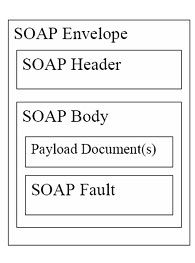
\includegraphics[scale=0.7]{img/schemasoap.png}
\caption{Struttura messaggio in SOAP}
\end{figure}

\paragraph{Esempi di Messaggi SOAP}
\begin{figure}[H]
\centering
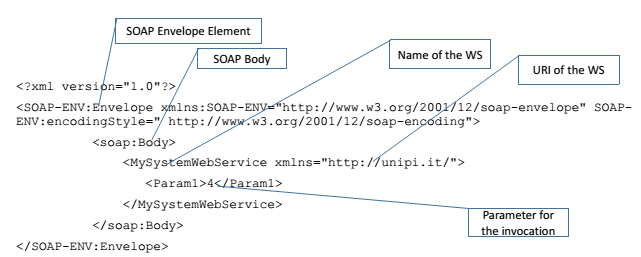
\includegraphics[scale=0.8]{img/soapRequest.png}
\caption{Richiesta}
\end{figure}

\begin{figure}[H]
\centering
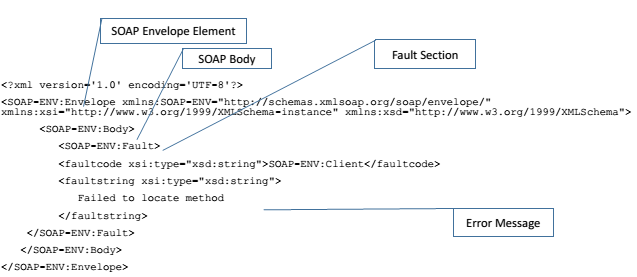
\includegraphics[scale=0.8]{img/soapResponse.png}
\caption{Risposta}
\end{figure}

\paragraph{WSDL}
Fornisce uno standard per l'interfaccia e il set di operazioni supportate da un servizio web. Stabilisce anche il set di parametri in input o output delle operazioni di un servizio ed il modo in cui i messaggi saranno trasferiti da/verso di esso. Tramite un documento WSDL un client può capire cosa fa un servizio, dove è locato e come può essere invocato. Ogni volta che il client deve utilizzare un servizio web sconosciuto, ne richiede il documento WSDL, lo analizza per ricavarne le informazioni necessarie ed infine invoca il servizio tramite SOAP.
\\ \\
Un messaggio WSDL è un documento XML composto da due sezioni:
\begin{itemize}
    \item \textbf{Service Interface Definition}: definisce in maniera astratta il servizio. Comprende alcune informazioni tra cui il \textit{tipo} del dato \xml{types}...\xml{/types}, i messaggi scambiati tra il provider ed il consumer (\xml{message}...\xml{/message}) e le operazioni che possono essere eseguite \xml{portTypes}...\xml{/portTypes>}.
    \item \textbf{Service Implementation Definition}: definisce in maniera più specifica come deve essere invocato il servizio \xml{service}...\xml{/service}, come trasferire i messaggi\\ \xml{binding}...\xml{/binding}
\end{itemize}

\begin{figure}[H]
\centering
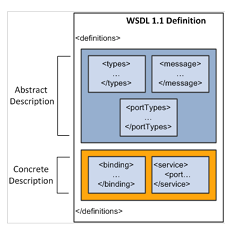
\includegraphics{img/WSDLMessage.png}
\caption{Struttura generica Messaggio WSDL}
\end{figure}

Andando ad analizzare più nel dettaglio i vari \textit{tag} che compongono un messaggio WSDL abbiamo:
\begin{itemize}
    \item \textbf{Types}: usato per definire tipi complessi per i dati usati poi nel messaggio.
        \begin{figure}[H]
        \centering
        \includegraphics[scale=0.8]{img/wsdlTypes.png}
        \caption{Struttura tag Types}
        \end{figure}
    \item \textbf{Message}: usato per definire il formato dei messaggi scambiati tra client e servizio web. Possono essere definiti sia messaggi di input che di output.
        \begin{figure}[H]
        \centering
        \includegraphics[scale=0.8]{img/wsdlMessageField.png}
        \caption{Struttura tag Message}
        \end{figure}
    \item \textbf{PortType}: usato per legare input ed output in un'operazione logica.
        \begin{figure}[H]
        \centering
        \includegraphics[scale=0.8]{img/wsdlPortTypes.png}
        \caption{Struttura tag PortType}
        \end{figure}
    \item \textbf{Binding}: usato per specificare come sono scambiati i messaggi associati ad una operazione \xml{PortType>}.
        \begin{figure}[H]
        \centering
        \includegraphics[scale=0.8]{img/wsdlBinding.png}
        \caption{Struttura tag Binding}
        \end{figure}
    \item \textbf{Service}: usato per specificare come un'operazione viene effettivamente invocata (tramite URI associato al servizio).
        \begin{figure}[H]
        \centering
        \includegraphics[scale=0.8]{img/wsdlServiceField.png}
        \caption{Struttura tag Service}
        \end{figure}
\end{itemize}

\paragraph{\textit{Universal Description, Discovery, Integration} (UDDI)} 
E' un protocollo indipendente dalle piattaforme utilizzate, basato su XML, che definisce un modo per pubblicare o scoprire informazioni sui servizi web. Usando l'UDDI un'azienda può registrare un WS ad un broker, mentre i client possono utilizzarlo per ricercare un certo WS e recuperarne le informazioni WSDL per poterlo poi invocare (tramite SOAP).

\paragraph{\textit{Representational State Transfer} (REST)}
Introdotto come alternativa più semplice per la creazione di servizi web, in quanto SOAP, richiedendo obbligatoriamente l'utilizzo di una struttura XML per lo scambio di messaggi, risultava essere un protocollo piuttosto complesso.
REST fornisce un modello per la progettazione di sistemi software \textit{network-based} che utilizza una struttura \textit{client/server} con protocollo HTTP per il trasferimento dei messaggi. \\
In un sistema RESTful, un client invia una richiesta usando i metodi standard di HTTP (\textit{PUT, GET, POST, DELETE}) ed il server invia una risposta che include la rappresentazione della risorsa specificata.
I dati sono ancora trasmessi usando XML come parte del contenuto del messaggio HTTP, ma tutto il markup addizionale richiesto da SOAP viene rimosso.


\subsection{Sistemi Distribuiti Message-oriented}
Le applicazioni cloud sono sviluppate come sistemi distribuiti la cui implementazione è la composizione di diverse funzionalità su differenti VMs. Queste VMs sono raggruppate in strati (tier), dentro ognuno di questi strati, per garantire alta disponibilità e scalabilità, le VMs replicano le loro funzionalità; le richieste dei client vengono ricevute dalle VMs nel primo strato (frontend tier) e successivamente inviate agli altri strati (backend tier). 
Viene utilizzata un'architettura "service oriented": ogni VM ospita uno o più componenti software autonomi che interagiscono con gli altri attraverso lo scambio di messaggi.

\begin{figure}[H]
\centering
\includegraphics[scale=0.5]{img/FeBe.PNG}
\caption{Architettura applicazioni cloud}
\end{figure}

Per la costruzione del servizio, ovvero per definire come vengono scambiati i messaggi, sono state definite due possibili soluzioni:
\begin{itemize}
    \item \textbf{SOAP:} usata per la comunicazione tra frontend e backend, ma molto raramente per la comunicazione tra client e frontend.
    \item \textbf{REST:} adottata spesso per la sua semplicità come interfaccia per l'utente quindi per la comunicazione tra client e frontend.
\end{itemize}

\begin{figure}[H]
\centering
\includegraphics[scale=0.5]{img/RestSoap.PNG}
\caption{Utilizzo SOAP e REST}
\end{figure}

Entrambe le soluzioni adottano un protocollo di comunicazione Request/Reply, per sfruttare le seguenti caratteristiche:
\begin{itemize}
    \item \textbf{Implementa comunicazione sincrona:} il client si blocca finchè non riceve la risposta dal server (time-coupled).
    \item \textbf{Affidabilità:} la risposta del server contiene un ACK della ricezione della richiesta.
    \item \textbf{Comunicazione diretta:} il client interagisce direttamente col server senza intermediari (space coupling) che implicherebbe un aumento di overhead e di complessità.
\end{itemize}
Il protocollo Request/Response va bene per la comunicazione tra client e frontend poichè soddisfa le richieste di semplicità e affidabilità e soprattutto perchè questo tipo di comunicazione può tollerare lo \textit{space/time coupling} ovvero il fatto che deve sempre sapere chi è il ricevitore e il ricevitore deve sempre essere attivo in quel preciso momento.
Per quanto riguarda la comunicazione tra frontend e backend il discorso è diverso. In questo caso è previsto che il backend abbia diverse VMs per supportare la scalabilità, grazie al load-balancing, e la disponibilità, grazie alle repliche dei dati.
Supportare questa dinamicità è di primaria importanza è un approccio space/time coupling non è adatto per garantire la scalabilità nella comunicazione nel backend (o nella comuncazione tra frontend e backend).
Ci serve allora un protocollo di comunicazione indiretta (introducendo un intermediario) per garantire:
\begin{itemize}
    \item \textbf{Space uncoupling:} il mittente non deve sapere per forza l'identità del ricevitore e viceversa; mittente e ricevitore possono quindi essere rimpiazzati, migrati, replicati al tempo di esecuzione.
    \item \textbf{Time uncoupling:} mittente e ricevitore hanno lifetime indipendenti, non c'è bisogno che siano attivi allo stesso momento per comunicare.
\end{itemize}
La caratteristica di \textit{Time uncoupling} è assicurata dall'intermediario che adotta un protocollo di comunicazione asincrono: il mittente invia i messaggi all'intermediario senza bloccarsi, e l'intermediario si occupa di consegnare i messaggi al destinatario.
\subsubsection{Comunicazione Message Oriented}
Per le applicazioni cloud sono stati definiti diversi paradigmi per la comunicazione indiretta orientata ai messaggi, in ognuno di questi, mittente e destinatario non aprono un canale di comunicazione diretto come connessioni TCP/UDP, ma piuttosto il mittente immette il messaggio in un bus che viene implementato da un intermediario.

\begin{figure}[H]
\centering
\includegraphics[scale=0.5]{img/Bus.PNG}
\caption{Bus di comunicazione}
\end{figure}

Sono stati definiti due tipi di intermediario: \textbf{Broker} o \textbf{Message Queue}.
\paragraph{Broker} 
Un sistema \textit{Publish-Suscribe} è un sistema dove i mittenti (publishers) "pubblicano" le strutture dati, solitamente un evento, e i destinatari (subscribers) esprimono interesse verso uno specifico dato attraverso sottoscrizioni. Al centro del sistema c'è il \textit{broker} che è responsabile di inoltrare i dati dai mittenti ai destinatari (abbina una sottoscrizione a un dato e garantisce la corretta consegna delle notifiche). 
Il tipo di comunicazione è \textit{one-to-many}.

\begin{figure}[H]
\centering
\includegraphics[scale=0.5]{img/Broker.PNG}
\caption{Architettura soluzione Message Broker}
\end{figure}

Ci sono diversi tipi di sottoscrizione:
\begin{itemize}
    \item \textbf{Channel-based:} il mittente pubblica i dati in un determinato canale e il destinatario sottoscrive uno di questi canali per ricevere tutti i dati inviati a quel canale.
    \item \textbf{Topic-based:} ogni dato ha un insieme di campi, uno di questi denota l'argomento (\textit{topic}) del dato. Le sottoscrizioni avvengono in base agli argomenti di interesse; approccio simile a quello visto prima con la differenza che nel caso del canale l'argomento è implicito mentre ora viene dichiarato esplicitamente.
    \item \textbf{Type-based:} le sottoscrizioni sono definite in base ai tipi di eventi.
\end{itemize}
\paragraph{Message Queue}
Le code di messaggi forniscono uno scambio di messaggi punto-punto tra il produttore e il consumatore: il mittente colloca il messaggio nella coda che viene poi rimosso dal destinatario. Questo approccio viene implementato grazie al \textit{Message Queueing System} che consente l'istanziamento di più code di messaggi.

\begin{figure}[H]
\centering
\includegraphics[scale=0.5]{img/MQS.PNG}
\caption{Architettura soluzione Message Queue}
\end{figure}

Il \textit{Message Queueing System} consente le seguenti operazioni:
\begin{itemize}
    \item \textbf{Invio:} eseguito dal produttore per collocare il messaggio nella coda.
    \item \textbf{Ricezione bloccante:} eseguita dal consumatore che si blocca finchè non è disponibile un messaggio appropriato.
    \item \textbf{Ricezione non bloccante (polling operation):} eseguita sempre dal consumatore per verificare lo stato della coda; restituisce un messaggio se ve ne sono di disponibili o, altrimenti, un'indicazione che nessun messaggio è disponibile.
    \item \textbf{Notifica:} eseguita dal \textit{Message Queueing System} per notificare al consumatore che è disponibile un messaggio nella coda a lui associata (il consumatore deve sottoscrivere i primi update in una certa coda).
\end{itemize}

\paragraph{Messaggi}
Ogni messaggio è composto da:
\begin{itemize}
    \item \textbf{Destinazione:} che è un identificatore univoco della coda di destinazione.
    \item \textbf{Metadati associati al messaggio:} includono campi come la priorità del messaggio e la modalità di consegna.
    \item \textbf{Corpo del messaggio.}
\end{itemize}
La politica di gestione della coda è FIFO, ma molte code supportano il concetto di priorità dei messaggi; il consumatore può anche selezionare i messaggi in base alle proprietà del messaggio.
Una delle proprietà più importanti dei messaggi è che sono \textbf{persistenti} ovvero che le code mantengono i messaggi finché non vengono consumati e affiderà i messaggi al disco per permettere una consegna affidabile.
Sui messaggi in arrivo può essere eseguita la trasformazione dei messaggi, l'uso più comune di questa operazione è per modificare il formato dei messaggi per gestire l'eterogeneità delle rappresentazioni dei dati. Il termine \textit{message broker} è spesso usato per denotare un servizio responsabile di trasformazione dei messaggi.
Le code di messaggi sono perfette per le comunicazioni lato backend dell'applicazione cloud poiché sono in grado di gestire la dinamicità che caratterizza questo ambiente (scalabilità). Per esempio sono in grado di gestire la variazione del numero delle VMs presenti in un determinato strato per far scalare il sistema, le VMs che implementano le stesse funzionalità riceveranno i dati dalla stessa coda essendo così in grado di garantire politiche come il bilanciamento del carico di lavoro e la disponibilità.

\begin{figure}[H]
\centering
\includegraphics[scale=0.5]{img/ScalaMQS.PNG}
\caption{Scalabilità delle code di messaggi}
\end{figure}

\subsubsection{Implementazione Message Broker e Message Queueing System}
I due metodi possono essere implementati sia in maniera centralizzata che distribuita.
Nel primo caso il \textit{broker} o il \textit{message queueing system} vengono implementati in un unico sistema (e.g. in un'unica VM). Questa implementazione è molto semplice e lineare ma manca di flessibilità e scalabilità visto che rappresenta un singolo punto di rottura per il sistema e un bottleneck per le performance.
Nel secondo caso invece viene implementata una rete di \textit{broker} o di \textit{message queueing system}, chiaramente è più complessa, poiché necessita di coordinazione tra i componenti e di repliche dei dati, ma garantisce flessibilità e scalabilità al sistema. 
Una delle implementazione più utilizzate per i \textit{message queueing system} è chiamata \textit{Advanced Message Queueing Protocol} (AMPQ).
\paragraph{Replica dei dati}
Nelle applicazioni cloud ogni strato include un gruppo di VMs che implementano le stesse funzionalità per fornire scalabilità, disponibilità e tolleranza ai guasti. Per assicurare che ogni VM lavori sullo stesso set di dati è richiesta una corretta replica dei dati tra le VMs dello stesso strato, per poter fornire lo stesso servizio ad ogni utente. Generalmente la replica dei dati viene implementata attraverso lo scambio di messaggi tra le VMs dello stesso cluster. Solitamente quando sono coinvolti dataset molto grandi viene usata una memoria condivisa che offre un set di dati comune che viene condiviso tra tutte le VMs; in questo caso lo scambio di dati diretto tra le VMs è limitato a messaggi per un corretto coordinamento.

\begin{figure}[H]
\centering
\includegraphics[scale=0.5]{img/Replica.PNG}
\caption{Replica dei dati}
\end{figure}

La replica dei dati tra più VMs deve tenere in considerazioni i seguenti requisiti:
\begin{itemize}
    \item \textbf{Trasparenza agli utenti:} gli utenti devono accedere a diverse copie dei dati senza esserne consapevoli.
    \item \textbf{Consistenza:} le repliche devono essere consistenti tra loro, la stessa operazione eseguita su ogni replica deve produrre lo stesso risultato.
    \item \textbf{Flessibilità:} il sistema deve essere elastico al fallimento di una VM.
\end{itemize}
\paragraph{Modello del sistema}
I dati nel sistema sono organizzati come una collezione di oggetti, come un file, una classe o un insieme di record; ogni oggetto logico è implementato come una collezione di copie fisiche di dati chiamate repliche. Ogni replica viene memorizzata in un diverso \textit{replica manager}, un componente che memorizza un'istanza della replica (nel nostro caso la VM), in questi \textit{replica manager} sono consentite le operazioni di aggiornamento sui dati in maniera recuperabile in modo tale che possono essere recuperate le inconsistenze sui dati dovute ad un fallimento.
Per garantire la consistenza, le repliche sono delle macchine a stati, che significa che oltre ai dati replicano anche uno stato.

\begin{figure}[H]
\centering
\includegraphics[scale=0.5]{img/RManager.PNG}
\caption{Rappresentazione \textit{replica manager}}
\end{figure}

\paragraph{Gestione delle richieste}
Una richiesta può essere:
\begin{itemize}
    \item \textbf{Una query:} non modifica lo stato dell'oggetto.
    \item \textbf{Un aggiornamento:} modifica lo stato dell'oggetto.
\end{itemize}
In generale per gestire una singola richiesta proveniente da un client vengono eseguiti i seguenti passaggi:
\begin{itemize}
    \item \textbf{Richiesta:} ricevuta da un modulo frontend che rilascia la gestione della richiesta a uno o più \textit{replica manager} (il modulo frontend può, in base all'implementazione scelta, comunicare direttamente con un solo \textit{replica manager}, che a sua volta comunicherà con gli altri, o con tutti i \textit{replica manager}).
    \item \textbf{Coordinazione:} i \textit{replica manager} si coordinano per prepararsi all'esecuzione della richiesta, possono decidere se eseguire la richiesta subito o posticiparla per imporre un ordine di esecuzione che mantenga la consistenza, la scelta dipende dal livello di ordinamento richiesto dal sistema (FIFO, causale o totale).
    \item \textbf{Esecuzione:} i \textit{replica manager} eseguono la richiesta, solitamente viene eseguita in maniera provvisoria così che può essere "disfatta" se ce n'è bisogno (per esempio per il recupero da un guasto).
    \item \textbf{Accordo:} i \textit{replica manager} cercano di raggiungere il consenso sugli effetti della richiesta (se necessario), se viene trovato il consenso l'esecuzione della richiesta viene "committata" e (se necessario) vengono applicate le relative modifiche.
    \item \textbf{Risposta:} uno o più \textit{replica manager} rispondono al frontend.
\end{itemize}
\paragraph{Comunicazione multicast}
Ci sono diversi metodi per consentire la comunicazione in multicast tra i quali:
\begin{itemize}
    \item \textbf{Atomic Multicast:} il messaggio viene consegnato a ogni membro che lo deve ricevere o a nessuno, eventuali perdite nella comunicazione vengono gestite, i duplicati vengono rimossi.
    \item \textbf{Total Order Multicast:} ogni membro deve ricevere tutti gli aggiornamenti nello stesso ordine.
    \item \textbf{Causal Order Multicast:} supponiamo che 'a' e 'b' siano due aggiornamenti, se 'a' avviene prima di 'b' allora ogni membro deve accettare prima 'a' di 'b'.
    \item \textbf{View-synchronous Communication:} tutti i membri vedono esattamente la stessa vista di ogni messaggio in ogni momento.
\end{itemize}
\subsubsection{Diversi approcci per la gestione delle repliche}
\paragraph{Passive or Primary-backup Replication}
Questo modello viene adottato per garantire tolleranza ai guasti, ad ogni istante un \textit{replica manager} viene selezionato come primario mentre gli altri fungono da backup. I frontend comunicano solo col \textit{replica manager} primario che è responsabile di gestire le richieste e inviare le copie dei dati aggiornati ai backup. Se il \textit{replica manager} primario cade, uno dei \textit{replica manager} di backup viene eletto come nuovo primario.

\begin{figure}[H]
\centering
\includegraphics[scale=0.5]{img/PassiveBackup.PNG}
\caption{Architettura \textit{Passive Replication}}
\end{figure}

Vediamo ora come vengono gestite le richieste in questo modello in accordo ai passaggi visti precedentemente:
\begin{itemize}
    \item \textbf{Richiesta:} il frontend invia una richiesta al \textit{replica manager} primario contenente un identificatore univoco della richiesta.
    \item \textbf{Coordinazione:} il \textit{replica manager} primario gestisce le richieste atomicamente nell'ordine in cui le ha ricevute senza il bisogno di coordinarsi con i \textit{replica manager} di backup, se la richiesta è già stata eseguita (stesso identificatore di una precedente) viene inviata la stessa risposta.
    \item \textbf{Esecuzione:} il primario esegue la richiesta e salva il risultato.
    \item \textbf{Accordo:} se la richiesta è un aggiornamento il \textit{replica manager} primario invia a tutti i \textit{replica manager} di backup lo stato aggiornato, la risposta e l'identificatore univoco; i backup inviano al primario un ACK (per queste comunicazioni si usa una comunicazione di tipo Atomic Multicast).
    \item \textbf{Risposta:} il \textit{replica manager} primario risponde al frontend che fa arrivare la risposta al client.
\end{itemize}
\paragraph{Active Replication}
\textit{Active Replication} è un approccio diverso che garantisce alta disponibilità. I \textit{replica manager} sono organizzati in gruppi, i frontend inviano le richieste in multicast a tutti i \textit{replica manager} del gruppo che processeranno la richiesta indipendentemente e invieranno tutti la stessa risposta. Se uno qualunque dei \textit{replica manager} cade, non c'è alcun impatto negativo nelle performance del sistema poichè tutti i \textit{replica manager} restanti sono in grado di rispondere alla richiesta.

\begin{figure}[H]
\centering
\includegraphics[scale=0.5]{img/ActiveReplication.PNG}
\caption{Architettura \textit{Active Replication}}
\end{figure}

Vediamo, anche questa volta, come vengono gestite le richieste in questo modello:
\begin{itemize}
    \item \textbf{Richiesta:} il frontend attacca alla richiesta un identificatore univoco per la stessa e la invia in multicast a tutti i \textit{replica manager}.
    \item \textbf{Coordinazione:} in questa fase non c'è bisogno di alcun coordinamento poiché il metodo multicast provvede a inviare la richiesta a tutti i \textit{replica manager}, il metodo di multicast adottato deve essere il \textit{Total Order Multicast} per garantire che le richieste vengano ricevute nello stesso ordine da tutt i \textit{replica manager}.
    \item \textbf{Esecuzione:} ogni \textit{replica manager} esegue la richiesta indipendentemente in maniera identica.
    \item \textbf{Accordo:} grazie all'uso del metodo \textit{Total Order Multicast} non c'è bisogno di questa fase.
    \item \textbf{Risposta:} ogni \textit{replica manager} invia la propria risposta al frontend, dato che tutte le risposte che riceverà il frontend saranno uguali, il frontend potrà inoltrare verso il client la prima risposta che riceve.
\end{itemize}
\paragraph{Gossip}
Quest'ultimo approccio è stato definito per fornire contemporaneamente sia alta disponibilità che scalabilità, concentrandosi nel fornire accesso al servizio ai clienti per il maggior tempo possibile. In particolare con questo approccio:
\begin{itemize}
    \item invece di inviare gli aggiornamenti appena sono disponibili, per raggiungere un accordo collettivo prima di restituire il controllo al client, l'invio degli aggiornamenti viene rimandato quando possibile per restituire il controllo al client il prima possibile.
    \item tutti i \textit{replica manager} sono coinvolti nella gestione delle richieste ricevute dal frontend.
\end{itemize}
Nella architettura \textit{Gossip} i \textit{replica manager} si scambiano messaggi di gossip periodicamente per trasmettere gli aggiornamenti che ricevono dai client. I client vengono assegnati a specifiche istanze di frontend per un corretto bilanciamento del carico di lavoro ma hanno comunque la possibilità di collegarsi ad una nuova istanza in caso di fallimento della precedente.
Il servizio fornisce essenzialmente due tipi di operazione:
\begin{itemize}
    \item \textbf{Query:} che sono operazioni \textit{read-only}.
    \item \textbf{Aggiornamenti:} che modificano lo stato dell'oggetto, queste operazioni non leggono lo stato dell'oggetto.
\end{itemize}
Il sistema \textit{Gossip} garantisce:
\begin{itemize}
    \item che ogni client ottenga un servizio consistente nel tempo, cioè, in risposta ad una query, i \textit{replica manager} forniscono una serie di dati che corrisponde agli ultimi aggiornamenti che il client ha osservato fino a quel momento.
    \item la consistenza tra le repliche può non essere rigida nel tempo a causa del frequente scambio di messaggi di gossip, quindi il client può ricevere un'informazione vecchia ma consistente quando emette una query; in altre parole viene garantita la consistenza sequenziale.
\end{itemize}

\begin{figure}[H]
\centering
\includegraphics[scale=0.5]{img/Gossip.PNG}
\caption{Architettura \textit{Gossip}}
\end{figure}

Vediamo come vengono gestite le richieste in questo modello:
\begin{itemize}
    \item \textbf{Richiesta:} il front end invia richieste ad un singolo \textit{replica manager} per volta.
    \item \textbf{Coordinazione:} il \textit{replica manager} che riceve la richiesta non la processa finché non può farlo in accordo ai vincoli di ordinazione richiesti.
    \item \textbf{Esecuzione:} il \textit{replica manager} esegue la richiesta.
    \item \textbf{Accordo:} i \textit{replica manager} aggiornano i dati tra loro grazie allo scambio di messaggi di gossip che conterranno l'ultimo valore che hanno ricevuto. Gli aggiornamenti vengono scambiati in modalità "pigra" ovvero vengono scambiati solo occasionalmente o dopo che hanno collezionato diversi aggiornamenti o quando un \textit{replica manager} scopre che gli manca un aggiornamento, che aveva precedentemente inviato ad un altro peer, per processare una richiesta. 
    \item \textbf{Risposta:} in caso di risposta ad una query, il \textit{replica manager} risponde al termine dell'esecuzione, se invece deve rispondere ad un aggiornamento lo fa subito dopo averlo ricevuto.
\end{itemize}
Per mantenere l'ordine temporale delle richieste vengono utilizzati i \textit{timestamp} (i frontend ovviamente devono avere i loro clock sincronizzati). In particolare ogni frontend conserva un vettore di \textit{timestamp} che rispecchia la versione degli ultimi valori dei dati, questi \textit{timestamp} vengono inviati al \textit{replica manager} (campo "prev" nell'immagine) insieme alla query. Il \textit{replica manager} risponde con un nuovo \textit{timestamp} (campo "new" nell'immagine) che verrà unito al timestamp generato dal frontend.

\begin{figure}[H]
\centering
\includegraphics[scale=0.5]{img/Timestamp.PNG}
\caption{Utilizzo \textit{timestamp}}
\end{figure}

Vediamo come viene processata una query. Il \textit{timestamp} associato a una query rispecchia l'ultima versione del valore che il frontend ha letto o inviato come aggiornamento, per questo motivo ogni volta che il \textit{replica manager} riceve una query deve rispondere con un \textit{timestamp} uguale o più recente di quello ricevuto nella query; se il \textit{timestamp} in possesso del \textit{replica manager} è più vecchio di quello della query la richiesta viene rimandata e messa nella lista delle richieste pendenti in attesa di ricevere l'aggiornamento che gli manca per inviarlo al frontend. \\ 
Per quanto riguarda il processamento di una richiesta di aggiornamento, quando il \textit{replica manager} la riceve dal frontend ne analizza il \textit{request ID} per controllare se la richiesta era già stata processata, se la richiesta è "nuova" il \textit{replica manager} crea un nuovo \textit{timestamp} incrementando il valore di \textit{prev} ricevuto e invia la risposta con il nuovo \textit{timestamp} allegato. Inoltre il \textit{replica manager} aggiunge una nuova entrata alla tabella delle operazioni di aggiornamento pendenti, se la condizione sui \textit{timestamp} è soddisfatta (\textit{timestamp} della risposta uguale o più recente di quello ricevuto nella query) l'operazione viene "committata" altrimenti viene rimandata finché la condizione non sarà soddisfatta (verrà verificata ogni volta che il \textit{replica manager} riceve un aggiornamento tramite i messaggi di gossip).
\subsubsection{ZooKeeper}
\textit{ZooKeeper} è un servizio ad alta disponibilità sfruttato solitamente per piccoli scambi di dati tra servizi, può essere usato anche per memorizzare informazioni sula configurazione, creare una directory distribuita o un sistema di denominazione. È un servizio replicato quindi per funzionare necessita che la maggioranza dei nodi non siano caduti (i server caduti vengono esclusi automaticamente e se tornano attivi possono essere ricongiunti). Utilizza lo schema \textit{Primary-backup} per la gestione delle repliche e implementa un protocollo denominato ZAB (ZooKeeper Atomic Broadcast).
\paragraph{ZAB}
\textit{Atomic Broadcast} è un sistema di messaggistica atomica che mantiene tutti i server sincronizzati, il sistema garantisce:
\begin{itemize}
    \item \textbf{Consegna affidabile:} se un messaggio m viene consegnato da un server, allora sarà consegnato da tutti i server.
    \item \textbf{Total Order:} se un messaggio a viene consegnato prima di un messaggio b da un server, allora sarà consegnato prima di b da ogni server.
    \item \textbf{Causal Order:} se un messaggio b viene inviato dopo che un messaggio a è stato consegnato, a deve essere ordinato prima di b; se un mittente invia c dopo aver inviato b, c deve essere ordinato dopo b.
\end{itemize}
Vediamo ora come funziona il protocollo:

\begin{figure}[H]
\centering
\includegraphics[scale=0.5]{img/Zab.PNG}
\caption{Funzionamento protocollo ZAB}
\end{figure}

Con:
\begin{itemize}
    \item \textbf{CEPOCH:} un \textit{follower} invia la sua ultima promessa al potenziale \textit{leader}.
    \item \textbf{NEWEPOCH:} il \textit{leader} propone una nuova epoca e'.
    \item \textbf{ACK-E:} ack del \textit{follower} per la nuova epoca proposta dal \textit{leader}.
    \item \textbf{NEWLEADER:} il \textit{leader} potenziale propone se stesso come nuovo \textit{leader} per l'epoca e'.
    \item \textbf{ACK-LD:} ack del \textit{follower} per il nuovo \textit{leader} proposto.
    \item \textbf{COMMIT-LD:} commit del nuovo \textit{leader} proposto.
    \item \textbf{PROPOSE:} il \textit{leader} propone una nuova transazione.
    \item \textbf{ACK:} ack del \textit{follower} per la proposta del \textit{leader}.
    \item \textbf{COMMIT:} il \textit{leader} committa la proposta.
\end{itemize}
\paragraph{Elezione del leader}
L'elezione avviene in due fasi:
\begin{itemize}
    \item inizialmente, viene eseguita l'elezione del \textit{leader} locale per trovare un \textit{leader} potenziale (può essere scelto in diversi modi, per esempio quello con l'ID o con l'indirizzo IP più "grande").
    \item successivamente, il \textit{leader} potenziale consolida il suo ruolo stabilendo una nuova epoca, ovvero un nuovo periodo in cui diventa il \textit{leader} se ottiene il consenso.
\end{itemize}
Il consolidamento del \textit{leader} avviene anch'esso in due fasi:
\begin{itemize}
    \item nella prima fase ogni \textit{follower} invia un messaggio \textbf{CEPOCH} contenente l'informazione sull'ultima epoca.
    \item nella seconda fase il \textit{leader} potenziale invia un messaggio \textbf{NEWEPOCH} contenente la proposta della nuova epoca basata sul quorum dei messaggi ricevuti dai \textit{follower}, questo messaggio viene accettato dai \textit{follower} con un messaggio di \textbf{ACK}.
\end{itemize}
Dopo aver proposto la nuova epoca, il \textit{leader} propone se stesso come nuovo \textit{leader} inviando messaggi \textbf{NEWLEADER}, anche in questo caso tutti i \textit{follower} accettano inviando messaggi \textbf{ACK}, dopo aver ricevuto gli \textbf{ACK} da tutti i \textit{follower} il \textit{leader} committa l'elezione di se stesso come \textit{leader} attraverso il messaggio \textbf{COMMIT-LD}. 
Ogni volta che un aggiornamento deve essere propagato ai \textit{follower}, il leader lo invia in un messaggio \textbf{PROPOSE} e, dopo aver ricevuto gli \textbf{ACK} da tutti, può inviare il messaggio \textbf{COMMIT} per committare l'aggiornamento.\\
Questo tipo di protocollo per assicurare la consistenza dei dati adotta il commit in due fasi.
\paragraph{Quorum e Consenso}
L'elezione del \textit{leader} utilizza il quorum per garantire una vista consistente del sistema: durante ogni operazione il \textit{leader} deve ottenere il consenso, ovvero la metà più uno dei \textit{follower} devono accettare la proposta del \textit{leader}. Se non viene raggiunto il quorum si verifica lo scenario \textit{split-brain}, questo scenario deve essere evitato, per questo è altamente suggerito costituire il sistema con un numero di nodi dispari in modo tale da assicurare che una maggioranza possa sempre essere raggiunta (che sia accettando o rifiutando la proposta).\\
In caso di partizionamento della rete (scenario \textit{split-brain}), alcuni dei nodi alcuni dei nodi non saranno in grado di comunicare tra loro perché risiederanno in frazioni di rete separate, questo può portare all'impossibilità di elaborare le richieste dell'utente o a modifiche inconsistenti dei dati. \textit{ZooKeeper} adotta un meccanismo per individuare:
\begin{itemize}
    \item fallimenti nelle comunicazioni tra i nodi.
    \item partizionamento della rete.
\end{itemize}
Se il cluster è stato suddiviso in diversi componenti indipendenti, ogni componente potrebbe pensare di essere una sorta di "cluster master" e di poter continuare a processare le richieste dell'utente portando ad un'inconsistenza dei dati. Per evitare che questo possa succedere, solo il componente con più nodi viene tenuto attivo mentre tutti gli altri vengono spenti.

\subsection{Load Balancing}
Pensiamo ad un'applicazione cloud su scala globale, disponibile a centinaia di milioni di utenti nel mondo (es. Google con 5,4 miliardi di richieste al giorno). I problemi principali da affrontare sono la scalabilità e la gestione del carico. Per questo è necessario disporre di un cluster di VM per operare il load balancing. Tuttavia, questa soluzione potrebbe non essere sufficiente in quanto il numero massimo di rischieste è comunque limitato dai vincoli fisici dell'infrastruttura di rete che serve per trasmettere i dati dai client alle VM.\\
Per mitigare questo \textit{bottleneck}, il cluster delle VM è sparso in diverse località del pianeta detti \textit{datacenter}, opportunamente dimensionati rispetto al numero di utenti in una determinata regione. Il risultato che si ottiene è una naturale suddivisione del carico in diverse località con diverse infrastrutture di rete.
\subsubsection{Approccio Globale e Locale}
Il bilanciamento del carico può essere operato a livello locale o globale:
\begin{enumerate}
    \item \textbf{Globale:} distribuisco le richieste attraverso diversi datacenter. Decido verso quale datacenter inoltrare la richiesta dell'utente in base ad un qualche criterio (es. distanza).
    \item \textbf{Locale:} dentro un determinato datacenter, decido quali VM servono una particolare richiesta. Solitamente mirato al bilanciamento del carico per ottenere scalabilità.
\end{enumerate}
Vediamo alcune \textbf{politiche di global load balancing}.
\paragraph{Soluzione con DNS}
Prima che il client invii una richiesta, deve scoprire l'indirizzo IP tramite il servizio DNS. Vogliamo sfruttare questa fase per introdurre un primo strato di distribuzione del carico. Una possibile soluzione potrebbe essere quella di far restituire al DNS più indirizzi IP per una singola richiesta: a questo punto sarà il client a sceglierne uno. Abbiamo così introdotto un primo livello di distribuzione del carico.\\
Tuttavia, questa soluzione offre pochissimo controllo sul comportamento del client il quale sceglie un indirizzo casualmente, senza prendere in considerazione la distanza (o altre metriche di costo). Per mitigare questo effetto si potrebbe pensare di utilizzare un indirizzo \textit{anycast}\footnotemark per il servizio DNS ma quello che vorremmo è una soluzione con un controllo \textit{fine-grained} (granulare?).
\footnotetext{: un indirizzo anycast è assegnato a più interfacce (host) diverse ma solo una di queste risponderà al client, tipicamente la più vicina.}
\paragraph{Soluzione con Virtual IP}
Un indirizzo IP virtuale è un indirizzo che non è assegnato ad un host/interfaccia in particolare ma è condiviso tra diversi servizi. Dal punto di vista dell'utente, il VIP è un indirizzo regolare, che nasconde tutti i dettagli implementativi.\\
Un set di VIP sono assegnati ad un'applicazione mentre un singolo VIP di questo set è assegnato ad una regione nella quale abbiamo più datacenter. Il DNS regionale configurerà il VIP come indirizzo per un determinato servizio in modo tale che gli utenti avranno un unico IP di riferimento. A questo punto il bilanciamento del carico verrà gestito da un \textit{global load balancer} che si occuperà di distribuire le richieste ai datacenter più adatti a rispondere in quel momento.\\
\begin{figure}[H]
    \centering
    \includegraphics[scale=0.5]{img/gre.png}
    \caption{Incapsulamento pacchetti e Tunnel GRE}
\end{figure}\noindent
Il global load balancer incapsulerà il pacchetto del client in un nuovo pacchetto IP che sarà spedito al datacenter. Quest'ultimo, aprirà il pacchetto e vi troverà al suo interno quello originale del client. In questo modo è come se il client avesse inviato il pacchetto direttamente al datacenter.\\
La comunicazione tra load balancer e datacenter viene gestita tramite un tunnel GRE (\textit{Generic Routing Encapsulation}) che permette di incapsulare pacchetti IP dentro altri pacchetti IP. In questo modo il \textit{global load balancer} può spedire il pacchetto attraverso un percoso preciso verso il datacenter più opportuno.\footnotemark \footnotetext{: se non incapsuliamo in un tunnel il pacchetto spedito dal global LB ritornerebbe in ingresso allo stesso global LB in quando l'IP destinatario del pacchetto è il VIP.}

\subsection{Consistenza e Affidabilità}
I sistemi cloud distribuiti su scala mondiale devono avere una visione consistente dello stato del sistema e dei dati attraverso molteplici siti. La replicazione e sincronizzazione dei dati è una sfida importante per i sistemi distribuiti in quanto:
\begin{itemize}
    \item la banda limitata influisce sul tempo necessario a sincronizzare i dati;
    \item l'affidabilità delle comunicazioni può influire sulla presenza o meno di partizioni di rete\footnotemark;
\end{itemize}
\footnotetext{: un nodo (o una porzione del sistema distribuito) può disconnettersi per un determinato periodo di tempo rimanendo isolato dal resto del sistema. Questo può causare un malfunzionamento parziale o totale del servizio in quanto avremo una partizione del nostro sistema isolata dall'altra.}
Per questi motivi, le strategie tradizionali di replicazione dei dati non sono adatte.

\subsubsection{Teorema CAP}
Un sistema distribuito può soddisfare contemporaneamente solo due delle seguenti proprietà:
\begin{itemize}
    \item \textbf{C}onsistency: tutti i nodi vedono gli stessi dati allo stesso istante.
    \item \textbf{A}vailability: il fallimento di un nodo non impedisce ai restanti di continuare a funzionare.
    \item  \textbf{P}artition-tolerance: il sistema continua a funzionare a prescindere dalle partizioni di rete.
\end{itemize}
Poichè soddisfare queste tre proprietà è impossibile, esistono solo tre tipologie di sistemi distribuiti:
\begin{itemize}
    \item \textbf{CP - Consistency \& Partitions}
    \item \textbf{AP - Availability \& Partitions}
    \item \textbf{CA - Consistency \& Availability}
\end{itemize}
\begin{figure}[H]
    \centering
    \includegraphics[scale=0.2]{img/cap.png}
    \caption{Combinazioni CAP}
\end{figure}\noindent
Questo non significa che un sistema \textbf{AP} sia inconsistente. Semplicemente da la priorità alla \textit{availability} in cambio di un "rilassamento" sulla consistenza. Stesso discorso vale per i sistemi \textbf{CP} in cui si cede un po' di \textit{availability} in cambio della piena consistenza.

\subsubsection{ACID vs BASE}
\paragraph{ACID}
Nei sistemi tradizionali i dati vengono memorizzati secondo la politica ACID:
\begin{itemize}
    \item \textbf{Atomicity:} il processo deve essere suddivisibile in un numero finito di unità indivisibili, chiamate transazioni. L'esecuzione di una transazione perciò deve essere per definizione o totale o nulla, e non sono ammesse esecuzioni parziali.
    \item \textbf{Consistency:} le transazioni lasciano i dati in uno stato consistente sia prima che dopo l'esecuzione.
    \item \textbf{Isolation:}  ogni transazione deve essere eseguita in modo isolato e indipendente dalle altre transazioni
    \item \textbf{Durability:} detta anche persistenza, si riferisce al fatto che una volta che una transazione abbia effettuato una \textit{commit}, i cambiamenti apportati non dovranno essere più persi.
\end{itemize}
Questi sistemi si concentrano prevalentemente sulla consistenza e, secondariamente, sulla disponibilità (availability). I sistemi ACID suppongono che le partizioni di rete siano "rare". In un sistema cloud su scala globale le partizioni di rete possono essere frequenti e ciascun nodo serve migliaia di utenti: le partizioni devono continuare a funzionare e a garantire il servizio. Per questo motivo l'approccio ACID non va bene.
\paragraph{BASE}
Acronimo di \textit{\textbf{B}asically \textbf{A}vailable \textbf{S}oft-state \& \textbf{E}ventual-consistency}, è una semantica recente ideata per sistemi che gestiscono grandi volumi di dati e che, pertanto, non possono avere un approccio ACID.\\
La novità principale introdotta da questo approccio è il concetto di Eventualmente Consistente: il sistema ed i suoi dati potrebbero essere inconsistenti per un breve periodo di tempo. Tuttavia, è garantito che la consistenza sarà raggiunta dopo un periodo di transizione.\\
La differenza principale rispetto alla semantica ACID è il modo in cui vengono gestite la query di update:
\begin{itemize}
    \item Nei sistemi ACID l'utente che esegue una scrittura attende che venga completata la propagazione dei nuovi dati.
    \item Nei sistemi BASE i dati vengono aggiornati immediatamente in locale e replicati nel resto del sistema in background in mariera asincrona.
\end{itemize}
\begin{figure}[H]
    \centering
    \includegraphics[scale=0.5]{img/acidvsbase.png}
    \caption{Esempio di sistema ACID (sopra) e BASE (sotto)}
\end{figure}\noindent
Ovviamente nei sistemi BASE possono verificarsi delle inconsistenze quando, ad esempio, un sito riceve una \textit{update} che va in conflitto con la copia locale dei dati. Per questi casi esistono dei procedimenti di risoluzione conflitti.

\subsubsection{Architettura Bayou}
E' un'architettura di tipo \textit{eventually-consistent} che fornisce repliche dei dati per alta \textit{availablity} ma poche garanzie sulla consistenza sequenziale.\\
Quando viene ricevuta una update, questa assume lo stato di \textit{tentative}. Finchè una update è \textit{tentative}, il sistema può annullarla o ri-eseguirla a seconda di cosa è necessario per raggiungere la consistenza.\\
Quando una update viene eseguita (commit), le modifiche rimangono applicate. In qualunque momento lo stato del sistema deriva dalla sequenza di update che sono state applicate, seguite dalla sequenza di update \textit{tentative}.
\begin{figure}[H]
    \centering
    \includegraphics[scale=0.4]{img/bayou.png}
    \caption{Sequenza in un sistema Bayou}
\end{figure}\noindent
Bayou adotta un sistema di commit primario: un replica manager viene scelto come primario e si assume la responsabilità di applicare (commit) le update. Se il replica manager primario si disconnette, il sistema continuerà a marcare le nuove update come \textit{tentative} in attesa che il primario torni online.\\
Per quanto riguarda il rilevamento e la risoluzione di conflitti sulle update, Bayou adotta due meccanismi:
\begin{itemize}
    \item \textbf{Dependency Check:} lo sviluppatore fornisce una \textit{query} e il corrispondente \textit{risultato atteso}. Se l'update, una volta eseguita, produce un risultato diverso da quello atteso si ha un conflitto.
    \item \textbf{Merge Procedure:} è una procedura che si attiva quando emerge un conflitto ed è fornita dagli sviluppatori.
\end{itemize}

\newpage
\section{Piattaforme Cloud}
\subsection{Piattaforme di Cloud Computing}
Le recenti tecnologie di virtualizzazione permettono di creare macchine virtuali al di sopra dell'hardware regolare: l'infrastruttura cloud sfrutta questo hardware non modificato per supportare la creazione delle macchine virtuali. Un gruppo di server si interconnettono tra loro attraverso un LAN ad alta velocità e si connettono a internet mediante un router. Questo gruppo di server e la LAN sono situati in un datacenter. Su ogni server è installato un hypervisor.\\
Un pool di server, che eseguono ognuno un hypervisor, sono uniti per creare una \textbf{piattaforma cloud}, un sistema distribuito che controlla gli hypervisor di tutti i server:
\begin{itemize}
    \item gestisce l'istanziazione/distruzione delle macchine virtuali: in ogni momento controlla quale macchine virtuali devono essere eseguite su un dato server e con quali proprietà.
    \item espone un'interfaccia di gestione in modo da permettere la gestione delle macchine virtuali: quest'interfaccia può essere usata dagli utenti per controllare la generazione delle macchine virtuali o da un software per automatizzarne il controllo.
    \item permette di implementare un modello cloud IaaS in quanto permette la creazione e distruzione delle macchine virtuali. Al di sopra di tale infrastruttura può essere impiegato un modello più complesso.
\end{itemize}

\subsubsection{Architettura Generale}
L'architettura generale delle piattaforme cloud è semplice:
\begin{itemize}
    \item un gruppo di server sono connessi a una LAN ad alta velocità.
    \item ogni server ha un sistema operativo installato su dell'hardware fisico.
    \item Un hypervisor è installato sul sistema operativo per virtualizzare le risorse fisiche offerte dal server.
    \item un software di piattaforma cloud viene installato per controllare le risorse locali virtualizzate dall'hypervisor (\textbf{agent} della piattaforma cloud).
    \item una particolare istanza del software di piattaforma cloud, chiamato \textbf{controller}, può essere installato su un server senza hypervisor o su una macchina virtuale ed è responsabile di controllare l'intera piattaforma comunicando con l'agent.
\end{itemize}

\begin{figure}[H]
    \centering
    \includegraphics[scale=0.5]{img/cp_architecture.png}
    \caption{Architettura Piattaforma Cloud}
\end{figure}\noindent

\subsection{OpenStack}
\textit{OpenStack} è una piattaforma software open-source per il cloud computing modello IaaS e è la soluzione principale adottata per il modello \textbf{privato} di cloud computing. Non richiede hardware particolarmente potente per funzionare. Il software è installato su ogni server e funziona sul sistema operativo dell'host; ognuno di questi server è chiamato \textbf{OpenStack Node}.\\
\textit{OpenStack}, sfruttando i singoli hypervisor, crea e distrugge le macchine virtuali.
La piattaforma gestisce la connessione delle macchine virtuali alla Rete Virtuale, utilizzata per comunicare con le altre macchine e con le reti esterne.
Inoltre essa gestisce lo spazio di archiviazione, questo permette la creazione di dischi rigidi virtuali da collegare alla macchina virtuale.

\begin{figure}[H]
    \centering
    \includegraphics[scale=0.5]{img/os_platform.png}
    \caption{OpenStack Piattaforma Software}
\end{figure}\noindent
I nodi che eseguono \textit{OpenStack} sono configurate per formare una singola \textbf{istanza di OpenStack} combinando insieme capacità di computazione, memoria e archiviazione per creare le macchine virtuali.\\
In una singola istanza almeno un nodo è configurato come \textbf{controller} che ha il compito di coordinare le funzioni di OpenStack e gestire le risorse dell'istanza. Gli altri nodi sono configurati come \textbf{nodi computazionali} che offrono le risorse per eseguire le macchine virtuali. \\
I nodi sono connessi attraverso una LAN ad altà velocità reale, utilizzata come
\begin{itemize}
    \item infrastruttura sulla quale creare le reti virtuali.
    \item rete di comunicazione tra i componenti di \textit{OpenStack}
\end{itemize}

\paragraph{Architettura di OpenStack}
La piattaforma offre:
\begin{itemize}
    \item una dashboard web per permettere a utenti e admin di gestire le risorse virtuali.
    \item un'interfaccia con riga di comando
    \item un'interfaccia basata su REST API, utilizzabili anche da programmi esterni.
\end{itemize}
\textit{OpenStack} è un software altamente modulare:
\begin{itemize}
    \item Le funzionalità della piattaforma sono raggruppate in servizi.
    \item Ogni servizio è implementato come un modulo diverso e separato.
    \item Ogni modulo può lavorare separatamente dalla piattaforma ed è sviluppato e mantenuto come un progetto separato.
\end{itemize}
Ogni servizio espone un set di REST API,attraverso questa interfaccia può ricevere richieste da utenti e admin attraverso un'interfaccia web o da riga di comando e da altri moduli. \\
I servizi si scambiano le operazioni di coordinazione e le informazioni di stato usando un sistema a coda di messaggi.
\begin{figure}[H]
    \centering
    \includegraphics[scale=0.25]{img/os_architecture.png}
    \caption{Architettura OpenStack}
\end{figure}\noindent

\paragraph{Servizi di OpenStack}
\textit{OpenStack} presenta dei servizi Core (Nova, Glance, Keystone), ovvero che sono mandatori ad ogni installazione, e servizi opzionali (per esempio Cinder, Neutron, ecc.), che vengono installati solo se le loro funzionalità sono richieste.\\
I servizi sono installati sul nodo controller o sui nodi computazionali a seconda delle funzionalità; alcuni devono esseri installati su entrambi i tipi di nodo con configurazioni diverse. \\
Tutti i servizi nel nodo controller sfruttano alcuni servizi di supporto: 
\begin{itemize}
    \item un \textbf{Database} per lo status e la configurazione dello spazio di archiviazione.
    \item un \textbf{Message Broker} per lo scambio di messaggi tra i diversi moduli.
\end{itemize}
All'interno della piattaforma, i servizi interagisco tra loro in tre modi diversi:
\begin{itemize}
    \item \textbf{Message Broker}: si scambiano un messaggio diretto attraverso il message broker.
    \item \textbf{REST API}: un servizio invoca l'interfaccia REST API nello stesso modo in cui lo farebbe un programma esterno.
    \item \textbf{DataBase}: due moduli si scambiano informazioni attraverso il database.
\end{itemize}           
\begin{figure}[H]
    \centering
    \includegraphics[scale=0.30]{img/info_exchange.png}
    \caption{Architettura OpenStack}
\end{figure}\noindent
% Nella parte finale del pacchetto D02 c'è altra roba su OpenStack quindi aggiungetela qua poi

\subsubsection{Keystone}
\textit{Keystone} è una componente per l'\textbf{identity management} ed è sfruttata da \textit{OpenStack} per l'\textbf{autenticazione} e l'\textbf{autorizzazione} ad alto livello: assicura la sicurezza concedendo o negando a Utenti diversi l'accesso agli oggetti.\\
Gli oggetti sono raggruppati in \textbf{progetti} e le autorizzazioni possono essere concesse in base ai progetti a cui un utente è assegnato.
Solitamente \textit{Keystone} è installato sul nodo controller.\\
L'autorizzazione di \textit{Keystone} è un'autorizzazione di tipo token-based: \begin{enumerate}
    \item l'utente interagisce con \textit{Keystone} autenticandosi con nome utente e password.
    \item se l'autenticazione ha successo l'utente riceve un token.
    \item il token viene usato per accede a tutti i servizi di OpenStack
    \item ogni servizio si occupa di validare il token.
\end{enumerate} 

\subsubsection{Nova}
\textit{Nova} è una componente per la \textbf{gestione delle macchine virtuali} ed è responsabile di istanziare e gestire le macchine virtuali. \textit{Nova} non implementa una nuova tecnologia di virtualizzazione, ma si interfaccia con gli hypervisor esistenti e può usare tecnologie di virtualizzazione diverse.\\
\textit{Nova} include due moduli diversi: nova controller installato sul nodo controller e il nova agent installato sui nodi computazionali.

\paragraph{Nova Controller}
Il componente nova del controller è responsabile di gestire le richieste degli utenti e le risorse disponibili sui nodi: colleziona le richieste di creazione o distruzione delle macchine virtuali dalle interfacce, valuta le azioni da compiere e le invia ai nodi computazionali.\\
Il modulo nova installato sul controller è composta da:
\begin{itemize}
    \item \textbf{Nova-API}: espone l'intrfaccia REST usata dagli utenti e dagli altri servizi.
    \item \textbf{Nova-Conductor}: gestisce le operazioni di controllo.
    \item \textbf{Nova-Scheduler}: valuta il giusto piazzamento per una nuova macchina virtuale a seconda dello stato dei nodi e delle risorse disponibili.
    \item \textbf{Nova-Network}: implementa i servizi network di base per le macchine virtuale e le interfacce.
    \item \textbf{Nova-Consoleauth e Nova-Novpcproxy}: implementano una console con cui gli utenti possono connettersi alle macchine virtuali.
\end{itemize}
Tutti le componenti interagiscono tramite coda di messaggi.

\paragraph{Nova Agent}
Nei nodi computazionali, la componente nova ha il compito di ricevere le istruzioni dal modulo controller e di tradurle in comandi per l'hypervisor.\\
Il nova agent è composto solo dal \textbf{compute service}: riceve i comandi dal controllo e istanzia o termina le macchine virtuali interagendo con l'hypervisor.
Nel nodo vengono mantenuti driver per interfacciarsi con diversi hypervisor e ogni driver espone un'interfaccia comune usata dal nova agent per interagire con gli hypervisor.

\paragraph{Workflow della Creazione delle Macchine Virtuali}
Quando arriva una richiesta per la creazione di una nuova macchina virtuale le componenti nova eseguono i seguenti passaggi:
\begin{enumerate}
    \item Nova-API riceve la richiesta e la passa al Nova-Conductor.
    \item Nova-Conductor passa la richiesta al Nova-Scheduler, che suggerisce il giusto piazzamento per la nuova macchina.
    \item Se il Nova-Scheduler permette la creazione della nuova macchina , il Nova-Conductor invia la richiesta al Nova-Network per istanziare la giusta configurazione di rete.
    \item La richiesta viene inviata al Nova-Compute del nodo selezionato dallo Scheduler.
    \item Il Nova-Compute locale interagisce con l'hypervisor per creare la macchina.
\end{enumerate}
\begin{figure}[H]
    \centering
    \includegraphics[scale=0.5]{img/vm_nova_creation.png}
    \caption{Creazione VM con Nova}
\end{figure}\noindent

La politica di schedulazione di \textit{Nova} può essere personalizzata per soddisfare diversi requisiti. Lo scheduler esegue una fase iniziale di filtraggio in cui gli host non adatti vengono rimossi e poi gli host rimanenti vengono ordinati secondo la politica scelta. La politica può essere configurata per includere certi gradi di impiego della RAM e della CPU.
\begin{figure}[H]
    \centering
    \includegraphics[scale=0.5]{img/nova_policy.png}
    \caption{Creazione VM con Nova}
\end{figure}\noindent

\subsubsection{Glance}
Le macchine virtuali sono solitamente costruite a partire da un'immagine-template di un hard drive virtuale, che include già un sistema operativo pre-installato e pre-configurato. \textit{Glance} è il servizio di gestione delle immagini di \textit{OpenStack}, gestisce le sopracitate immagini. Quindi, gli utenti possono caricare queste immagini pre-configurate da installare sulle proprie macchine virtuali. \\
Le immagini possono anche essere "personalizzate", per andare a includere set di software che saranno pronti all'uso una volta installata l'immagine. \\
\textit{Glance} è formato da 2 sottocomponenti: 
\begin{itemize}
    \item \textbf{Glance:} per la gestione delle istanze. Espone l'interfaccia (REST API) agli altri moduli e all'utente. Salva la lista delle immagini disponibili e le relative feature nel DB.
    \item \textbf{Glance Storage:} è responsabile di memorizzare le immagini/template sul disco. È nascosto all'utente, comunica soltanto con l'immagine Glance. Supporta differenti opzioni di storage, attraverso differenti driver:
    \begin{itemize}
        \item Un file system locale disponibile nella macchina in cui Glance è in esecuzione.
        \item Un file system cloud.
    \end{itemize}
\end{itemize}
Questo servizio Glance, tipicamente viene installato nel nodo controller. In definitiva, questo componente è responsabile di salvare i template delle macchine virtuali con cui le stesse macchine virtuali verranno create.
\begin{figure}[H]
    \centering
    \includegraphics[scale=0.3]{img/glance architecture.png}
    \caption{Architettura Glance}
\end{figure}\noindent

\subsubsection{Neutron}
Componente responsabile di creare e gestire network virtuali. I \textit{Virtual Network}, quindi, avranno il compito di collegare macchine virtuali, anche se quest'ultime girano su nodi differenti. \\
\textit{Neutron} non solo gestisce il network virtuale, ma inoltra il traffico tra macchine virtuali differenti. Quindi, sostanzialmente, fornisce una gestione completa della rete virtuale. \\
Il \textit{Local Physical Network} che interconnette i nodi, è sfruttato da Neutron per implementare la rete virtuale. In generale, come già visto nella teoria della virtualizzazione, per virtualizzare una risorsa, tipicamente ne serve una "fisica". Questo principio, quindi, è valido anche per il network. 
\begin{figure}[H]
    \centering
    \includegraphics[scale=0.2]{img/neutron local physical.png}
    \caption{Neutron - Local Physical Network}
\end{figure}\noindent
Le funzionalità di Neutron sono implementate in una modalità distribuita, ed è formato da due sottocomponenti:
\begin{itemize}
    \item \textbf{Neutron-Server:} installato nel nodo \textit{controller}. È responsabile della gestione del network virtuale coordinando i \textit{Neutron-Agent} che girano nei nodi computazionali. È inoltre responsabile di esporre le API REST per la creazione e successiva gestione, da parte degli utenti, del network virtuale.
    \item \textbf{Neutron-Agent:} è un set di sotto-componenti. Installato uno per ogni \textit{nodo computazionale}. Sono responsabili di gestire il traffico tra le macchine virtuali, che girano, appunto, sui nodi computazionali. In maniera specifica, spedisce il traffico diretto a/generato da la macchina virtuale locale in modo da emulare differenti network virtuali che si estendono su differenti nodi computazionali. I dati sono spediti sulla \textit{Local Physical Network}. L'agent deve assicurarsi dell'isolamento tra le differenti macchine virtuali.
\end{itemize}
\begin{figure}[H]
    \centering
    \includegraphics[scale=0.5]{img/neutron subcomponents.png}
    \caption{Neutron - Sottocomponenti}
\end{figure}\
Nell'immagine d'esempio: se la VM2 volesse inviare un pacchetto alla VM4 (che sono parte della stessa rete virtuale), invierà questo pacchetto al \textit{Neutron Agent} del nodo compute in cui è ospitato e questo si preoccuperà di inviarlo al \textit{Neutron Agent} della VM4, questo si preoccuperà di recapitare il pacchetto alla suddetta VM.

\paragraph{Nodo Network} 
I network virtuali sono tipicamente network privati. \textit{Neutron} consente alle macchine virtuali di essere connesse al reti "esterne", quindi di essere connesse ad internet e rese accessibili quest'ultimo. \\ 
Per poter connettere una rete virtuale a Internet, deve essere istanziato un nodo Network. \\
Un \textit{Nodo Network} è un nodo (che tipicamente corrisponde al controller) che è connesso ad un network esterno (attraverso Internet) oltre alla rete locale che connette i nodi di \textit{OpenStack}. Per ridurre il numero di server nella rete, il Nodo Network può essere costruito direttamente in un nodo controller, ma non necessariamente deve esserlo. L'importante è che questi nodi non eseguano VM, perché le loro risorse devono essere dedicate alla gestione. \\
Questo nodo fa girare un agente particolare, chiamato \textbf{Neutron-L3-Agent}, che è responsabile di fare il rerouting del traffico da/a la network virtuale privata a/da la rete pubblica. Questa funzionalità è effettuata andando a istanziare router virtuali, che hanno il compito di implementare il routing del traffico e la funzionalità NAT. \\ 
In più, il Nodo Network ospita anche un modulo chiamato \textbf{Neutron-DHCP-Agent}, che ha il compito di gestire l'assegnamento della configurazione della rete alle macchine virtuali.
\begin{figure}[H]
    \centering
    \includegraphics[scale=0.5]{img/neutron network node.png}
    \caption{Neutron - Network Node}
\end{figure}\noindent
Possono essere associati indirizzi IP pubblici alle macchine virtuali. I router virtuali ai bordi della rete virtuale si preoccuperanno di implementare la \textit{Network Address Translation (NAT)}. La piattaforma consente di assegnare dinamicamente IP pubblici, attraverso un meccanismo di \textit{Floating IP address}. 
\begin{figure}[H]
    \centering
    \includegraphics[scale=0.5]{img/neutron virtual network.png}
    \caption{Neutron - Virtual Network}
\end{figure}\noindent

\paragraph{Physical Network Infrastructure}
Una tipica infrastruttura di rete \textit{OpenStack}, connessa ad una rete esterna, tipicamente è configurata con 3 differenti reti fisiche:
\begin{itemize}
    \item Una rete di gestione, utilizzata per la comunicazione dei servizi OpenStack.
    \item Una rete interna alle macchine virtuali, utilizzata per gestire la comunicazione tra le differenti macchine virtuali.
    \item Una rete esterna, per l'accesso Internet.
\end{itemize}
Le reti di management e la rete interna alle macchine virtuali possono essere implementate sulla stessa LAN fisica. Soltanto un nodo, il nodo Network, deve essere connesso alla rete esterna. \\
Il nodo controller può essere connesso solo alla rete di management.
\begin{figure}[H]
    \centering
    \includegraphics[scale=0.5]{img/neutron physical network.png}
    \caption{Neutron - Physical Network}
\end{figure}\noindent
Il Neutron Agent installato su ogni nodo computazionale, è altamente configurabile. Sono possibili differenti configurazioni, sfruttando differenti tecnologie per processare e inoltrare il traffico. \\ 
Una delle ultime versioni sfrutta \textit{OpenVSwitch} per implementare le funzionalità della rete locale e inoltrare il traffico tra nodi computazionali e il nodo network. OpenVSwitch consente di riconfigurare rapidamente il comportamento di ogni agente, seguendo le direttive del nova server.
\begin{figure}[H]
    \centering
    \includegraphics[scale=0.5]{img/neutron agent.png}
    \caption{Neutron Agent}
\end{figure}\noindent

\subsubsection{OpenVSwitch}
OVS è un'implementazione open-source di un uno switch di rete virtuale distribuito. Progettato specificatamente per fornire uno stack "switching" per ambienti di virtualizzazione hardware, può girare all'interno del (o insieme a) l'hypervisor, per gestire il traffico da/a le macchine virtuali. Supporta l'implementazione del filtering, routing, switching e manipolazione dei pacchetti (in accordo a delle regole pre-stabilite). \\
Adotta un approccio centralizzato (SDN): ogni nodo ha la sua istanza OVS, che è controllata da un \textit{controller}. Seguendo le direttive del controller, tutte le istanze OVS implementano uno switch virtuale distribuito.
\begin{figure}[H]
    \centering
    \includegraphics[scale=0.5]{img/openvswitch.png}
    \caption{OpenVSwitch}
\end{figure}\noindent

\paragraph{Software Defined Networking (SDN)}
OVS adotta il paradigma SDN: le regole di rete sono configurate dinamicamente su ogni istanza basandosi sulle direttive che arrivando dal controller centralizzato. Ogni nodo OVS ha una tabella (flow table) che descrive le feature di ogni pacchetto in ingresso (l'indirizzo IP del mittente, l'indirizzo MAC di destinazione ecc..) e il la corrispondente azione che deve essere intrapresa (inoltrare il pacchetto, modificare il pacchetto ecc...) \\
Ogni volta che un pacchetto è ricevuto, si accede alla tabella e se il pacchetto ha un match con una delle entry della tabella, si esegue la corrispondente azione. Se non si trova un match, OVS manda un messaggio di query al controller, il quale risponde con una nuova regola che deve essere aggiunta nella tabella locale o una specifica azione che deve essere eseguita una volta sola. \\
Il protocollo che implementa la comunicazione tra le istanze OVS e il controller è chiamato \textit{OpenFlow}.
\begin{figure}[H]
    \centering
    \includegraphics[scale=0.9]{img/sdn.png}
    \caption{Software Defined Networking}
\end{figure}\noindent

\paragraph{Comunicazione VM - OVS}
Ogni macchina virtuale ha un NIC virtuale, il cui hardware è emulato dall'hypervisor. Per potersi connettere con l'istanza di OVS del nodo computazionale, il vNIC è connesso ad un altro NIC virtuale creato nel sistema operativo dell'host (tap0, tap1). \\
Un \textit{tap} è un'interfaccia di rete virtuale che può essere collegata con un software, in questo caso l'hypervisor, per ricevere/inviare il traffico di rete (frames di layer 2) da/al software. Il tap, quindi, è usato per ricevere/inviare traffico di dati da/a la macchina virtuale. Il traffico dalle interfacce tap è gestito da OVS per implementare le funzionalità di routing e forwarding.
\begin{figure}[H]
    \centering
    \includegraphics[scale=0.5]{img/tap.png}
    \caption{Comunicazione VM - OVS}
\end{figure}\noindent

\paragraph{Nodo Network}
Le istanze OVS possono essere programmate dal server Neutron per spedire i dati tra differenti macchine virtuali che sono implementate sullo stesso nodo computazionale o su diversi nodi. Quando i dati sono diretti verso una rete esterna, invece, è spedita al nodo network. \\ 
Per implementare le funzionalità di routing e gestione dei dati a livello 3, si installa un'istanza di OVS nel nodo network. Attraverso questa istanza, le funzionalità di routing a livello 3 sono implementate per inoltrare il traffico da/a la rete esterna e la macchina virtuale (o in generale, la rete virtuale locale).
\begin{figure}[H]
    \centering
    \includegraphics[scale=0.5]{img/network node architecture.png}
    \caption{Network Node}
\end{figure}\noindent

\paragraph{Network Virtualization}
Network Virtualization è il processo con cui le Virtual Network (VN) per le macchine virtuali sono create sulla stessa infrastruttura fisica. \\
Le reti virtuali sono reti di layer 2, specificatamente reti Ethernet. L'implementazione di questo tipo di reti è la seguente:
\begin{itemize}
    \item Forwarding dei dati a livello 2 tra macchine virtuali che appartengono alla stessa rete virtuale.
    \item Isolamento tra reti virtuali. Ovvero, due macchine virtuali appartenenti a differenti reti virtuali non possono comunicare, a meno che non ci sia un router che connette il layer 3 delle due reti virtuali.
\end{itemize}
In OpenStack, la virtualizzazione della rete richiede che il traffico sia inoltrato tra differenti nodi computazionali e da/a il nodo network in accordo alla rete virtuale. Se due nodi computazionali hostano due macchine virtuali, che appartengono alla stessa rete virtuale, il servizio di rete dovrebbe essere configurato in modo tale da forwardare il traffico tra di loro. Con questo scopo, ogni pacchetto dovrebbe essere marcato con l'ID della rete virtuale a cui appartiene in modo tale che possa essere gestito correttamente. Vengono applicate tecnologie già esistenti come il tagging dei pacchetti e il tunneling.
\begin{figure}[H]
    \centering
    \includegraphics[scale=0.5]{img/network virtualization.png}
    \caption{Network Virtualization}
\end{figure}\noindent
VLAN è una delle più utilizzate per la virtualizzazione della rete. Lo standard di rete \textit{IEEE 802.1Q Ethernet} è stato definito specificatamente per consentire la creazione di LAN virtuali su reti Ethernet normali. \\
Con questo scopo, lo standard aggiunge nuovi campi nell'header di Ethernet, l'\textbf{ID (VID)}, che specifica l'ID della LAN virtuale a cui appartiene. Uno switch (virtuale o fisico) che supporta \textit{IEEE 802.1Q} è responsabile sia di aggiungere il campo \textbf{VID} quando un pacchetto è iniettato nella rete e sia di rimuoverlo quando raggiunge la destinazione. Per esempio, frame broadcast devono essere consegnati soltanto agli host che appartengono allo stesso VID, per garantire isolamento.
\begin{figure}[H]
    \centering
    \includegraphics[scale=0.4]{img/802.1Q.png}
    \caption{IEEE 802.1Q}
\end{figure}\noindent
\textit{Neutron} può essere configurato per usare VLAN per creare reti virtuali. Quando si costruisce una rete virtuale per connettere 2 o più macchine virtuali, il Nova Server assegna un \textit{VID} alla rete virtuale. \\
Il server configura l'OVS del nodo computazionale, in modo da taggare il traffico proveniente da una macchina virtuale, con il VID assegnato alla sua rete virtuale e per inoltrare il traffico a tutti i nodi computazionali coinvolti. \\
Nel caso in cui, la rete virtuale sia connessa a Internet attraverso un Virtual Router o che abbia un servizio DHCP attivato, il Server Neutron configura OVS sul nodo network in modo da taggare i pacchetti che arrivano/diretti al router/DHCP assegnato alla rete virtuale.
\begin{figure}[H]
    \centering
    \includegraphics[scale=0.4]{img/Neutron VLAN.png}
    \caption{Neutron VLAN Operation}
\end{figure}\noindent

\subparagraph{GRE Tunneling}
Un altro meccanismo di virtualizzazione adottato è il tunneling dei pacchetti attraverso il protocollo \textbf{Generic Routing Encapsulation (GRE)}. \\
\textit{GRE} è un protocollo di tunneling che consente di incapsulare pacchetti IP all'interno di altri pacchetti IP. Il protocollo è utilizzato per creare un tunnel tra due host internet. Aggiunge un header addizionale \textit{GRE}, per specificare il tipo di protocollo incapsulato. \\
GRE può essere utilizzato come meccanismo per creare reti virtuali: un tunnel GRE è creato per ogni coppia di nodi computazionali che hanno macchine virtuali che appartengono a specifiche reti virtuali (e tra il nodo computazionale e il nodo network). \\
Differenti ID per differenti tunnel GRE sono utilizzati per ogni rete virtuale. 
\begin{figure}[H]
    \centering
    \includegraphics[scale=0.4]{img/GRE tunneling.png}
    \caption{GRE Tunneling}
\end{figure}\noindent
GRE può essere utilizzato per creare reti virtuali. Per ogni rete virtuale, il Server Nova istanzia un nuovo \textit{GRE ID}. Quest'ultimo istruisce le istanze OVS per creare un adattatore di rete virtuale \textit{(gre-1)}, sopra l'interfaccia fisica. L'interfaccia GRE è responsabile di creare il tunnel tra i nodi computazionali coinvolti (nodi che hanno almeno una macchina virtuale che appartiene alla rete virtuale, o nodi computazionali e il Server della rete) e incapsulano/decapsulano il traffico.
\begin{figure}[H]
    \centering
    \includegraphics[scale=0.4]{img/Neutron GRE.png}
    \caption{Operazioni Neutron - GRE}
\end{figure}\noindent

\subparagraph{VXLAN}
Le VLAN hanno un limite, dato che gli identificatori VLAN sono da 12 bits. Quindi, il numero massimo possibile di VLAN è 4094. \\
Nelle implementazioni con un grande numero di cloud, anche se grande, questo può essere un problema.
\textbf{Virtual Extensible LAN (VXLAN)} è una tecnologia di virtualizzazione di rete che tenta di risolvere il problema di scalabilità associata a grandi deployment di cloud. Cerca quindi di rimuovere il limite di cui si è parlato precedentemente. \\
Con VXLAN si possono avere fino a 16 milioni di differenti reti virtuali. È sempre una metodologia di incapsulamento dei pacchetti tra due endpoints, chiamata \textit{Virtual Tunnel Endpoints (VTE)}. \\
I frames sono incapsulati in pacchetti UDP (non più a livello 2), mentre al livello IP sono specificati la sorgente e la destinazione dei VTE. \\
Un header VXLAN (che ha più di 12 bits) è incluso ogni volta che si crea un pacchetto VXLAN, per riportare l'ID della LAN virtuale. Dato che, due VTE possono supportare multiple VLAN allo stesso tempo, si usa l'ID quindi per distinguere la VXLAN.
\begin{figure}[H]
    \centering
    \includegraphics[scale=0.5]{img/VXLAN.png}
    \caption{VXLAN}
\end{figure}\noindent
I tunnel VXLAN sono utilizzati da Neutron alla stessa maniera in cui vengono utilizzati i tunnel GRE. Per ogni rete virtuale, viene istanziato un nuovo ID VXLAN dal Server Nova. Quest'ultimo istruisce le istanza OVS di incapsulare pacchetti nei tunnel VXLAN in accordo alle istanze delle reti virtuali.
\begin{figure}[H]
    \centering
    \includegraphics[scale=0.4]{img/Neutron e VXLAN.png}
    \caption{Neutron e VXLAN}
\end{figure}\noindent

\subsubsection{Cinder}
\textit{Cinder} è il componente responsabile della gestione di \textbf{volumi}. Ogni macchina virtuale ha un hard drive di default in cui è salvato il sistema operativo. Se una macchina virtuale richiede uno storage aggiuntivo, possono essere dinamicamente creati volumi addizionali di storage e aggiunti ad un'istanza. Questi volumi sono visti come hard drive virtuali dalla macchina virtuale. \\
Un hard drive virtuale è salvato nel file system come un'immagine (un file o un oggetto). \\
\textit{Cinder} è responsabile della gestione di queste immagini e di esporle alle macchine virtuali. Un hard drive virtuale è esposto dall'hypervisor, che accede agli hard drive virtuali attraverso il protocollo \textit{iSCSI}. \\
\textbf{iSCSI} (si prouncia aiscasi) è uno standard di archiviazione di rete basato su protocollo Internet che fornisce accesso a livello di blocco all'archiviazione.
Cinder salva le immagini di volume nel file system locale del nodo in cui il servizio è installato, oppure in un file system cloud.
\begin{figure}[H]
    \centering
    \includegraphics[scale=0.5]{img/Cinder.png}
    \caption{Cinder}
\end{figure}\noindent
\paragraph{Architettura di Cinder}
Cinder comprende i seguenti componenti:
\begin{itemize}
    \item \textit{Cinder-Api:} espongono un'interfaccia REST ai clients per controllare le operazioni Cinder (Nova o direttamente gli utenti finali),
    \item \textit{Cinder-Volume:} è responsabile di gestire direttamente le richieste dall'interfaccia REST.
    \item \textit{Cinder-Scheduler:} è responsabile di selezionare lo storage adeguato per salvare i nuovi drive (se ci sono più storage configurati sul sistema).
    \item \textit{Cinder-Backup:} è responsabile di creare backup di volumi esistenti quando sono richiesti dall'utente.
\end{itemize}
\begin{figure}[H]
    \centering
    \includegraphics[scale=0.4]{img/Architettura Cinder.png}
    \caption{Architettura Cinder}
\end{figure}\noindent

\subsubsection{Ceilometer}
Ceilometer è un componente di telemetria. Monitora tutti i componenti dell'istanza, misurando le risorse che vengono utilizzate da ogni utente. I dati che vengono raccolti da Ceilometer possono essere utilizzati per scopi di fatturazione. Monitora, inoltre, componenti telemetrici che possono essere usati per controllare lo stato del sistema.
\begin{figure}[H]
    \centering
    \includegraphics[scale=0.4]{img/Celiometer.png}
    \caption{Ceilometer}
\end{figure}\noindent
\paragraph{Architettura di Celiometer}
Ceilometer ha un \textit{Ceilometer-Collector} centralizzato, che è responsabile di ricevere tutti i dati dagli altri componenti di \textit{OpenStack} e di salvarli in un Database (tipicamente un database NoSQL tipo \textit{MongoDB}). Per collezionare dati dai nodi computazionali, si installa un \textit{Ceilometer-Agent} su ogni nodo. L'agente è responsabile di collezionare tutte le notifiche da tutti i componenti locali e inoltrarli al collector. \\
Il collector può esporre un set di API REST per recuperare i dati dal database.
\begin{figure}[H]
    \centering
    \includegraphics[scale=0.5]{img/Ceilometer architecture.png}
    \caption{Architettura Ceilometer}
\end{figure}\noindent

\subsubsection{Horizon}
Le funzionalità di \textit{OpenStack} sono esposte agli utenti attraverso una interfaccia web. La dashboard tipicamente è esposta dal controller. Consente la gestione di tutti gli aspetti delle istanze e fornisce un set di tools da linea di comando per la gestione backend.
\begin{figure}[H]
    \centering
    \includegraphics[scale=0.6]{img/Horizon.png}
    \caption{Horizon}
\end{figure}\noindent

\subsubsection{API di servizio}
Ogni servizio di \textit{OpenStack} espone un set di API, tutte le API di comunicazione sono REST. Le API vengono esposte da ogni servizio per l'interazione fra servizi e per esporre un set di funzionalità agli utenti. Queste API possono essere sfruttate dagli utenti per integrare il processo di automazione in applicazioni esterne.\footnote{\url{http://developer.openstack.org/api-ref.html}}
\begin{figure}[H]
    \centering
    \includegraphics[scale=0.5]{img/Service API.png}
    \caption{Service APIs}
\end{figure}\noindent

\subsubsection{Swift}
Swift è il servizio di storage di oggetti disponibile in \textit{OpenStack}. Consente agli utenti e agli altri moduli di OpenStack di salvare dati (rappresentati come oggetti), nella piattaforma Cloud. Gli altri servizi, come per esempio \textit{Cinder} o \textit{Glance}, possono utilizzare Swift per salvare rispettivamente backup di volumi o immagini. \\
Il componente è responsabile di gestire tutti gli aspetti dello storage di dati, dal ricevere e salvare i dati fino al recupero. I dati sono tipicamente salvati nello storage cloud, per garantire scalabilità. \\
Swift è composto da 2 componenti:
\begin{itemize}
    \item \textit{Swift-Proxy}: è responsabile di esporre l'interfaccia REST e gestire richieste (salvare un nuovo oggetto o recuperare un oggetto).
    \item \textit{Swift-Storage-Node}: che è installato su ogni "Nodo Storage" (un nodo che hosta una parte di dati), per salvare i dati su un disco fisico
\end{itemize}
\begin{figure}[H]
    \centering
    \includegraphics[scale=0.5]{img/swift.png}
    \caption{Swift}
\end{figure}\noindent

\subsubsection{Heat}
Heat è l'orchestratore di \textit{OpenStack}. Può gestire la creazione o la distruzione di VM o le loro impostazioni automaticamente. Questa automazione è basata su un set di regole che specificano quando devono triggerare azioni da effettuare sulla VM. \\
Attraverso Heat, per esempio, si può creare un servizio di autoscaling per sfruttare i dati riferiti allo status da Ceilometer per creare o distruggere VM in riferimento allo stato del sistema. \\
Il componente è composta dai seguenti moduli:
\begin{itemize}
    \item \textit{Heat-API}: espone l'interfaccia agli utenti per configurare l'orchestratore.
    \item \textit{Heat-Engine}: che è responsabile di gestire le richieste degli utenti e implementarle.
\end{itemize}
\begin{figure}[H]
    \centering
    \includegraphics[scale=0.5]{img/heat.png}
    \caption{Heat}
\end{figure}\noindent

\begin{figure}[H]
    \centering
    \includegraphics[scale=0.4]{img/openstack summary.png}
    \caption{Riassunto dell'interazione dei servizi di OpenStack}
\end{figure}\noindent

\subsubsection{High Availability (HA)}
L'architettura attuale include soltanto una istanza dei componenti di gestione. \textit{OpenStack} può essere installata nella cosiddetta configurazione ad alta disponibilità, ovvero è possibile distribuire più istanze di ciascun servizio al fine di garantire elevata disponibilità ed elasticità. Questo può essere effettuato in una maniera simile, le applicazioni cloud sono implementate in una maniera ridondante per garantire alta disponibilità. \\
Nella configurazione ad alta disponibilità, vengono distribuite multiple istanze di nodi controller con tutti i corrispondenti servizi, per controllare lo stesso set di nodi computazionali.
\begin{figure}[H]
    \centering
    \includegraphics[scale=0.3]{img/high availability 1.png}
    \caption{High Availability}
\end{figure}\noindent
\paragraph{Alta Disponibilità con nodi dedicati}
Le API di OpenStack sono esposte non direttamente dal nodo controller ma attraverso un Proxy di alta disponibilità. Questo Proxy è responsabile di ricevere le richieste e inoltrarle a uno dei nodi controller. \\
Il Proxy deve implementare funzionalità per rilevare quando avviene un fallimento dei nodi Controller, per rimuoverli dalla lista dei nodi attivi. \\ 
Lo storage State deve essere replicato tra i nodi controller.
\begin{figure}[H]
    \centering
    \includegraphics[scale=0.3]{img/high availability 2.png}
    \caption{High Availability con nodi dedicati}
\end{figure}\noindent
\paragraph{Alta Disponibilità con ridondanza semplice}
Le API di OpenStack sono esposte direttamente da un controller, selezionato come controller Master. \\
Le funzionalità del Proxy di alta disponibilità sono implementate su tutti i controller, uno di quelli è marcato come attivo e serve richieste, mentre gli altri sono marcati come inattivi. Le istanze del Proxy ad alta disponibilità devono coordinarsi per rilevare fallimenti e triggerare la riconfigurazione quando è necessaria. \\ 
Di nuovo, lo storage State deve essere replicato tra i nodi controller.
\begin{figure}[H]
    \centering
    \includegraphics[scale=0.3]{img/high availability 3.png}
    \caption{High Availability con ridondanza semplice}
\end{figure}\noindent
\newpage
\subsection{Piattaforme Cloud Computing leggere per DevOps}
\subsubsection{Development del Software - PRIMA}
Alcuni anni fa, la maggior parte delle applicazioni software erano grossi monoliti, che giravano come un singolo processo o un piccolo numero di processi. Avevano dei tempi di rilascio molto lenti e avevano degli aggiornamenti poco frequenti dato che il development era complesso e poco pratico: i developer solitamente confezionavano l'intero sistema e lo consegnavano al team operativo, il team o gli amministratori responsabili di gestire le infrastrutture (i server). Cambiare una parte dell'applicazione richiedeva il redesign dell'intera applicazione. \\
Nel tempo poi, la mancanza di confini tra i componenti software aumenta la complessità della progettazione e manutenzione, andando quindi a deteriorare la qualità dell'intera applicazione. Le applicazioni monolitiche spesso richiedono un piccolo numero di server alimentati. \\
Questi suddetti sistemi, vengono chiamati "legacy" e sono installati e funzionanti anche oggi (anche se sono sostituiti piano piano). Se conviene sono stati "cloudificati", ovvero i server fisici sono stati sostituiti da VM. Questo processo va a semplificare il processo di manutenzione dell'infrastruttura, anche se l'implementazione del software e la sua manutenzione è ancora complessa. \\
Quando l'applicazione deve avere a che fare con un carico crescente, si aggiungono risorse al server, ovvero si va ad utilizzare una scalabilità verticale e in questo modo non si va a modificare l'architettura originale dell'applicazione. Lo scaling verticale, però, ha dei limiti che non lo rendono sempre fattibile.
\subsubsection{Development del Software - ADESSO}
Il Cloud Computing ha radicalmente cambiato il modo in cui le applicazioni software sono progettate e implementate. Le grandi applicazioni monolitiche precedenti, adesso sono frammentate in componenti indipendenti, chiamati \textit{servizi} o \textit{microservizi}. \\ 
I servizi sono disaccoppiati dagli altri e possono essere progettati, implementati, aggiornati e scalati individualmente. Ogni servizio/microservizio gira come un processo indipendente e comunica con le altre componenti attraverso delle interfacce ben definite. \\
Questa struttura consente un ciclo di vita dell'applicazione molto più rapido: i componenti possono essere cambiati velocemente e facilmente, tutte le volte che è necessario per stare dietro ai rapidi cambiamenti dei requisiti aziendali. \\
I servizi comunicano attraverso un protocolli sincroni (SOAP, HTTP/RESTful) o in maniera asincrona attraverso lo scambio di messaggi (ad esempio code di messaggi). Tali protocolli sono semplici e ben conosciuti dai programmatori. \\
I servizi possono essere implementati separatamente, un cambiamento in uno di essi non comporta cambiamenti o la necessità di  re-implementarne altri (posto che le interfacce non cambino). \\
Questa nuova architettura ha inoltre cambiato l'intero processo di implementazione di un'applicazione e, in particolare, come le applicazioni sono gestite e distribuite in produzione. Nel passato, il ciclo di vita dell'applicazione era gestito da:
\begin{itemize}
    \item Il \textbf{team di Development (dev team)}: i cui task erano di progettare e programmare il software dell'applicazione.
    \item Il \textbf{team Operativo (ops team)}: che si prende cura di distribuire e di manutenere l'applicazione. 
\end{itemize}
Adesso le organizzazioni stanno adottando un approccio differente: lo stesso team che progetta l'applicazione si occupa anche di distribuirla e della manutenzione per tutto il ciclo di vita. Questo approccio viene chiamato \textit{DevOps}.

\subsubsection{DevOps}
Il principale vantaggio di questo approccio è quello di avere i programmatori più coinvolti nell'esecuzione dell'applicazione durante la produzione. Questo porta ad avere una maggior consapevolezza dei bisogni dell'utente e dei problemi nella progettazione dell'applicazione. \\
Il processo di distribuzione è semplificato: nel senso che le release possono essere fatte più spesso: idealmente si possono avere programmatori che distribuiscono la propria applicazione autonomamente senza avere il team ops coinvolto (implementazione continua). Questa pratica, però, richiede ai programmatori di avere una conoscenza profonda dei dettagli dell'infrastruttura sottostante, il che non è sempre possibile o desiderabile.

\subsubsection{NoOps}
Anche se i programmatori e gli amministratori di sistema lavorano per raggiungere tutti lo stesso obiettivo, tipicamente hanno background, esperienze e motivazioni differenti. Anche se il modello DevOps è considerato un target per i suoi vantaggi, la sua implementazione è difficile perché i membri del team dev difficilmente avranno il background e l'esperienza necessaria per gestire l'infrastruttura. \\
Una soluzione ideale potrebbe essere quella di mettere in pratica un approccio \textit{NoOps}, in cui i programmatori implementano l'applicazione da soli, senza conoscere nulla riguardo l'infrastruttura e senza avere a che fare con le peculiarità di distribuire l'applicazione. \\
Una soluzione per abilitare automaticamente la gestione e la manutenzione potrebbe rendere fattibile implementare un approccio DevOps o NoOps. Si potrebbe comunque avere bisogno di avere un team ops per gestire l'infrastruttura, ma ai programmatori dovrebbe essere consentito di distribuire il loro software facilmente.

\paragraph{Distribuzione e gestione dei servizi}
Indipendentemente dalla conoscenza richiesta per la distribuzione e gestione, un'architettura basata su servizi ha altri inconvenienti. \\
Quando un'applicazione è composta da un piccolo numero di componenti, la loro gestione è semplice. Quando il numero di componenti cresce, la complessità delle operazioni di distribuzione aumenta. \\  
La configurazione manuale e la distribuzione è noiosa, prona ad errori e non fattibile quando il numero di servizi raggiunge un certo numero. Una soluzione per l'automazione della distribuzione e della configurazione dei componenti è richiesta per gestire applicazioni grandi con un gran numero di servizi. 
\subparagraph{Dipendenze tra servizi}
Come già detto, i servizi sono implementati come componenti separati in maniera indipendenti da teams differenti. Data la loro indipendenza, è comune avere teams differenti usare librerie differenti. Ogni team seleziona la sua libreria e quando accade di selezionare la stessa libreria, potrebbe accadere che si vadano a selezionare versioni differenti della stessa. In più, differenti teams vorrebbero avere la libertà di sostituire la libreria quando ce n'è la necessità. Quindi, andare ad implementare differenti servizi/applicazioni con dipendenze incrociate potrebbe essere un incubo per il team ops.
\begin{figure}[H]
    \centering
    \includegraphics[scale=0.4]{img/dipendenze tra servizi.png}
    \caption{Dipendenze tra servizi}
\end{figure}\noindent

Indipendentemente dal numero di singoli componenti, uno dei maggiori problemi che gli sviluppatori e i team operativi hanno, è quello di affrontare le differenze nell'ambiente in cui eseguono le applicazioni. Un metodo per semplificare questo tipo di operazioni è quello di distribuire applicazioni in un ambiente ideale e confinato dove tutte le librerie sono pre-installate e il vero hardware su cui il software sta girando è in qualche modo astratto. \\ 
Questo ambiente può essere creato attraverso la full-virtualization, quindi andando a far girare il software in una macchina virtuale. Questa soluzione, tuttavia, è costosa, dato che la full-virtualization ha un overhead significativo. In più, utilizzando la VM, si ha un overhead in termini di configurazione della VM stessa dell'OS guest, per configurarla e installare le librerie necessarie.

\subsubsection{Virtualizzazione leggera}
I meccanismi di virtualizzazione leggera, come ad esempio i container, possono essere una soluzione a questo alto overhead richiesto dalla virtualizzazione "full". \\
I container possono essere usati per preparare un ambiente virtualizzato in cui le librerie e le dipendenze sono pre-installate e configurate per far girare una certa applicazione o un servizio, parte di un'applicazione. \\ 
In più i container possono essere facilmente spediti e installati su differenti macchine utilizzando un sistema di distribuzione ad-hoc che si prende cura di distribuire e installare le immagini su differenti macchine. Un esempio di questo è \textit{Docker}.

\subsection{Kubernetes}
Kubernetes è un sistema software implementato da \textit{Google}, consente di implementare e gestire facilmente applicazioni containerizzate su di esso. \\ Un'applicazione containerizzata è un'applicazione i cui componenti (servizi indipendenti) sono distribuiti e spediti come contaniner differenti. \\
Kubernetes mira a semplificare completamente il processo generale di distribuzione e gestione dei container che compongono l'applicazione, occupandosi degli aspetti relativi alla scalabilità, tolleranza agli errori, gestione delle risorse, ecc. L'obiettivo è quello di offrire un'infrastruttura IaaS leggera per distribuire le applicazioni in un modo semplice ed efficace, cosicché i programmatori possono occuparsene senza pensare ad altri aspetti. \\ 
Il team operativo è sempre richiesto, in questo caso, tuttavia, è responsabile di mantenere e far girare l'infrastruttura di Kubernetes. \\
Kubernetes è una piattaforma distribuita composta da un nodo \textbf{master} e un numero variabile di nodi \textbf{worker}. I nodi di Kubernetes possono essere installati direttamente sui server fisici o possono essere installati su piattaforme cloud su macchine virtuali. \\
Il nodo \textit{master} di Kubernetes espone un'interfaccia ai programmatori, quest'ultimi possono richiedere di eseguire una specifica applicazione. Il programmatore deve solo inviare un descrittore dell'applicazione, che contiene soltanto la lista dei componenti che compone l'applicazione. E per ogni componente, si specifica la configurazione. Quindi, il \textit{master} di Kubernetes si prende cura di distribuire i componenti dell'applicazione sui nodi \textit{worker}, in accordo alla descrizione fornita dal programmatore in maniera totalmente automatica. \\
Attraverso l'interfaccia, il programmatore può specificare che alcuni servizi devono girare insieme, conseguentemente sono implementate sullo stesso nodo \textit{worker}. Gli altri saranno divisi tra i cluster in accordo allo stato di ogni nodo. 
\begin{figure}[H]
    \centering
    \includegraphics[scale=0.4]{img/kubernetes.png}
    \caption{Kubernetes}
\end{figure}\noindent
In più alla configurazione di ogni componente, il programmatore deve specificare il numero desiderato di istanze in modo da assicurare la scalabilità. La piattaforma si prenderà cura di replicare ogni componente e di bilanciare il carico del traffico tra loro, per assicurare scalabilità. La piattaforma poi, monitorerà lo stato di ogni componente e gestirà i fallimenti: in caso di fallimento di un'istanza (o fallimento del nodo \textit{worker} su cui è eseguita) la piattaforma si preoccupa di replicare l'istanza con una nuova.

\paragraph{Vantaggi di Kubernetes}
Kubernetes toglie ai programmatori l'impegno dell'implementazione di funzionalità legate all'infrastruttura. La piattaforma si prende cura di implementare funzionalità come lo "scaling", il bilanciamento del carico e un meccanismo di auto-riparazione. Conseguentemente, i programmatori possono concentrarsi sulla progettazione dell'applicazione senza perdere tempo per capire come integrare l'applicazione nell'infrastruttura. \\
I compiti del team operativo sono, invece, alleggeriti: non si devono più preoccupare della distribuzione dei componenti, configurarli e successivamente risolvere i fallimenti, quelle funzionalità sono gestite dalla piattaforma stessa. In più, Kubernetes può ottenere un miglior utilizzo delle risorse disponibili nell'infrastruttura. 

\paragraph{Architettura del Cluster}
Il nodo \textit{master} implementa il \textit{piano controllo}, che è responsabile di controllare il cluster. Ogni componente del piano controllo può essere installato su un singolo nodo master, oppure splittato tra nodi differenti o replicato per garantire alta affidabilità. 
\begin{figure}[H]
    \centering
    \includegraphics[scale=0.4]{img/architettura kubernetes.png}
    \caption{Architettura Kubernetes}
\end{figure}\noindent
Il \textit{piano controllo} ha i seguenti componenti:
\begin{itemize}
    \item \textbf{API server:} espone l'interfaccia ai programmatori.
    \item \textbf{Scheduler:} schedula le applicazioni.
    \item \textbf{Controller manager:} effettua funzionalità a livello di cluster, come la replica dei componenti e gestione dei fallimenti dei nodi.
    \item \textbf{Etcd:} che è un componente per salvare dati in maniera affidabile.
\end{itemize}
I nodi \textit{workers}, invece, includono i seguenti componenti:
\begin{itemize}
    \item \textbf{Container runtime:} un ambiente runtime di container (come Docker, ad esempio) che si preoccupa di far girare i container.
    \item \textbf{Kublet:} che parla con il server API e gestisce i container sul nodo.
    \item \textbf{Kubernetes Service Proxy:} che si preoccupa di bilanciare il traffico di rete tra i componenti dell'applicazione e inoltra richieste, mentre i container sono migrati tra i nodi "working".
\end{itemize}

\paragraph{Distribuzione dell'applicazione}
La descrizione dell'applicazione fornita dal programmatore, mette in lista i container che compongono l'applicazione. I container sono raggruppati in \textbf{pods}. \\
Un \textit{pod} è un gruppo di container che devono girare sullo stesso nodo \textit{worker}, in altre parole devono essere distribuiti insieme e non dovrebbero essere isolati (un pod può essere un container). Per ogni pod o singolo container, il programmatore deve specificare la configurazione e il numero di repliche che devono essere distribuite.
\begin{figure}[H]
    \centering
    \includegraphics[scale=0.3]{img/kubernetes deployment.png}
    \caption{Deployment di Kubernetes}
\end{figure}\noindent
Dopo aver inviato il descrittore al piano controllo del nodo \textit{master}, lo scheduler schedula il numero specificato di repliche di pods al numero di nodi \textit{worker} disponibili. I \textit{Kublet} che girano sui nodi \textit{worker} si occupano di controllare \textit{Docker} per fare la pull delle immagini dei container dalla repository e farli girare.

\paragraph{Gestione e Manutenzione}
Una volta che l'applicazione sta girando, Kubernetes si occupa di controllare continuamente che lo stato dell'applicazione distribuita vada sempre a matchare con la descrizione fornita dai programmatori. \\
Se una o più istanze spettono di girare correttamente (crash dell'applicazione), Kubernetes li riavvierà. Se l'istanza o l'intero nodo diventano inaccessibili, Kubernetes selezionerà un nuovo nodo per tutti i container che giravano su quel nodo. \\
Mentre l'applicazione sta girando, il programmatore può decidere di aumentare o diminuire il numero di istanze, in questo caso la piattaforma può preoccuparsi di aggiungere o rimuovere istanze a runtime. Il programmatore può anche lasciar decidere alla piattaforma il numero ottimale di istanze per un certo container, in questo caso la piattaforma aggiusterà il numero di istanze basandosi su metriche real-time, come ad esempio il carico della CPU, consumo di memoria, query per secondi ecc...

\paragraph{Migrazione del Container}
La piattaforma si occupa automaticamente di istanziare container e migrarli quando è richiesto (per esempio quando un nodo fallisce). \\
Quando un container fornisce un servizio ad un client esterno, la piattaforma deve occuparsi di inoltrare le richieste al container che è stato spostato. Quello che è tipicamente fatto, è che viene esposto uno specifico servizio con un singolo indirizzo IP pubblico, nonostante il numero di container e la loro posizione. La piattaforma, con il componente \textit{kube-proxy} si preoccupa di connettere i container e inoltrare il traffico in maniera corretta. In più, il componente si occupa di implementare policy di bilanciamento del carico per inoltrare il traffico in maniera bilanciata per assicurare la scalabilità.

\paragraph{Esporre applicazioni}
I pods sono connessi a una rete locale privata, in modo per consentire la comunicazione tra di loro. Ogni pod ottiene il proprio indirizzo IP, tuttavia questo indirizzo è interno a questa rete e non è accessibile dall'esterno. Queste reti private locali consentono la comunicazione tra container che girano sullo stesso o su differenti nodi \textit{workers}. \\
Se un servizio ha bisogno di essere esposto a una rete esterna (perché, ad esempio, espone un'interfaccia web o le API REST dell'applicazione), il programmatore deve definire un \textit{oggetto servizio.} \\
Un \textit{oggetto servizio} istruisce la piattaforma per associare con un pod un indirizzo IP esterno e la relativa porta, cosicché il servizio esposto dal pod possa essere raggiunto dagli host esterni. Il servizio si prenderà cura di inoltrare le richieste che arrivano dall'indirizzo IP esterno all'indirizzo IP locale di una delle istanze pod associate. 
\begin{figure}[H]
    \centering
    \includegraphics[scale=0.3]{img/kubernetes esporre applicazioni.png}
    \caption{Esporre le applicazioni}
\end{figure}\noindent

\paragraph{Bilanciamento del carico}
Un servizio può essere connesso ad un pod che richiede multiple istanze ridondanti per il bilanciamento del carico. In questo caso il servizio diffonde le richieste tra le differenti istanze. Ad ogni pod della piattaforma associa un controller di replica per assicurarsi che il giusto numero di istanze sia correttamente in esecuzione.
\begin{figure}[H]
    \centering
    \includegraphics[scale=0.3]{img/kubernetes load balancing.png}
    \caption{Load Balancing di Kubernetes}
\end{figure}\noindent

\paragraph{Gestione dei fallimenti}
Il controller di replica è anche responsabile di monitorare le istanze di un pod per rilevare fallimenti. Se il fallimento di un nodo \textit{worker} è rilevato, il controller di replica lo rileva e reagisce andando a creare una nuova istanza pod.
\begin{figure}[H]
    \centering
    \includegraphics[scale=0.4]{img/kubernetes gestione fallimenti.png}
    \caption{Gestione fallimenti di Kubernetes}
\end{figure}\noindent

\paragraph{Pod design}
La regola generale per raggruppare container in pod è che il programmatore dovrebbe sempre eseguire i container in pod separati, a meno che non ci sia una specifica ragione che richieda che siano parte dello stesso pod, quindi vengono distribuiti sullo stesso nodo \textit{worker}. \\
Per esempio, un'applicazione potrebbe avere richieste di latenza nello scambio di dati tra 2 container, in questo caso è conveniente raggrupparli nello stesso pod, così non saranno obbligati a comunicare nella rete.
\begin{figure}[H]
    \centering
    \includegraphics[scale=0.3]{img/Kubernetes pod design.png}
    \caption{Pod design di Kubernetes}
\end{figure}\noindent

\newpage
\section{Infrastrutture Cloud e Meccanismi}
\subsection{Cloud Storage}
Il modello di memorizzazione dei dati di un sistema di calcolo tradizionale consiste in uno o più hard-drive collegati ad un solo server. Il problema degli hard-drive è che possono fallire e, in media, hanno un ciclo di vita di circa 5 anni. Per gestire il fallimento di un server viene utilizzata la tecnologia \textbf{RAID} (\textit{Redundant Array of Independent Disks}) che può assicurare repliche e tolleranza dei fallimenti.

\paragraph{RAID} E' una tecnologia che combina hard-drive multipli in uno o più hard-drive logici virtuali. Queste funzionalità possono essere implementate via hardware grazie ad un RAID controller al quale sono collegati i dischi fisici, oppure via software.
\begin{itemize}
    \item Hardware: il RAID controller gestisce gli hard-drive e, di conseguenza, le sue funzionalità sono nascoste al SO che accede solo al drive logico.
    \item Software: le funzionalità RAID sono implementate dal SO che gestisce l'accesso ai dischi fisici e la creazione dell'unità logica.
\end{itemize}

\begin{figure}[H]
    \centering
    \includegraphics[scale=0.7]{img/raid.jpg}
    \caption{Schemi RAID}
    \label{fig:raid}
\end{figure}\noindent
In figura \ref{fig:raid} sono riportati gli schemi RAID più popolari. In particolare, lo schema 0 è adottato per massimizzare le prestazioni ma non offre replica dei blocchi. Lo schema 1 massimizza la ridondanza a scapito delle prestazioni. Lo schema 5 propone una soluzione di compromesso tra la 0 e la 1: vengono introdotti dei blocchi di parità (ottenuti tramite XOR tra due blocchi) che vengono salvati su dischi diversi rispetto a quello calcolato (es. il blocco di parità 1 ottenuto come \( A \otimes B \) viene salvato sul disco 3).\\ \\
Nonostante le ottimizzazioni introdotte da RAID, la capacità di memoria massima è limitata dal numero fisico di slot per hard-drive sul server. In particolare, i requisiti di memorizzazione delle piattaforme cloud sono diversi da quelli dei sistemi tradizionali. Il requisito principale è la scalabilità della memoria ovvero vogliamo avere un supporto di memorizzazione che si adatta alla quantità di dati immagazzinati.

\subsubsection{File System Distribuito}
Approccio inventato per superare la limitazione imposta dal numero di slot fisici su un server. Con questo approccio abbiamo il FS di un server distribuito su più server in modo da estendere la sua memoria grazie alla memoria di un altro server.
\paragraph{GlusterFS} Tecnologia che crea un DFS mettendo insieme tutte le capacità di memorizzazione dei nodi disponibili. Non c'è distinzione tra client e server: tutti i nodi partecipano offrendo una parte della propria memoria locale. \textit{GlusterFS} è altamente configurabile con diversi livelli di ridondanza e repliche.
Un altro motivo per il quale vogliamo implementare un sistema di memorizzazione condiviso è la possibilità di usare la \textbf{VM Live Migration}. Si tratta di una tecnica che consente di spostare una macchina virtuale in maniera dinamica da un nodo all'altro, il tutto mentre è in esecuzione. Questa tecnica richiede per forza un sistema di memorizzazione condiviso altrimenti la VM dovrebbe essere spenta e l'hard-drive che la contiene dovrebbe essere fisicamente spostato da un server all'altro introducendo un \textit{downtime} significativo.

\paragraph{Storage Area Network} Una SAN è una rete ad alta velocità di dispositivi di memorizzazione ad alta capacità. Non sono server "classici" bensì dispositivi di memoria \textit{ad-hoc} connessi ai server che formano la piattaforma cloud. In questo modo creiamo un sottolivello di memorizzazione ad uso dei server. La comunicazione fra Server e SAN sarà gestita da protocolli \textit{ad-hoc}.\\
Il fatto che richieda soluzione hardware \textit{ad-hoc} rende le tecnologie SAN complesse e costose, per questo motivo non tutte le piattaforme cloud se lo possono permettere. Per questo motivo esistono altre tecnologie che si propongono per offrire un sistema di memorizzazione unificato, scalabile, performante e poco costoso (basato quindi su hardware general-purpose). Una delle più popolari al momento è Ceph.

\subsection{Ceph}
Ceph fornisce un sistema di memorizzazione robusto, affidabile e di livello \textit{enterprise} costruito sopra ad un set di \textit{Hard Drives} di tipo \textit{commodity} (quindi di basso costo/uso comune). Gestisce autonomamente le repliche dei dati e il recupero dai fallimenti. Non c'è più bisogno di impiegare tecnologie quali il RAID. Può essere installato su dei server normali per creare un DFS (detto anche Ceph cluster) in cui la capacità di tutti gli hard-drive è messa a disposizione.

\subsubsection{Architettura}
Un sistema Ceph è composto da nuemrosi servizi software separati fra loro, ciascuno che si occupa di una diversa funzionalità. I client (che possono essere applicazioni o servizi cloud) interagiscono con questi servizi software.
\begin{figure}[H]
    \centering
    \includegraphics[scale=0.3]{img/ceph.jpg}
    \caption{Architettura Ceph}
\end{figure}\noindent
Al centro di Ceph abbiamo \textbf{RADOS} (\textit{Reliable Autonomic Distributed Object Store}) il quale è responsabile della memorizzazione degli oggetti. Il livello RADOS fa si che i dati rimangano sempre in uno stato consistente e affidabile, esegue le repliche dei dati, rilevamento dei fallimenti \& recupero e bilanciamento dei dati redistribuendo tra i nodi del cluster. Un'applicazione che vuole interagire con RADOS può farlo grazie ad una libreria (LIBRADOS) che fornisce un'interfaccia nativa disponibile per diversi linguaggi di programmazione.\\
I servizi di RADOS sono:
\begin{itemize}
    \item \textbf{OSD} \textit{(Object-based Storage Device)}: In Ceph tutto è salvto sotto forma di oggetti (anche di dimensioni enormi) secondo un approccio replicato.
    \item \textbf{MON} \textit{(Ceph Monitor)}: è responsabile per monitorare lo stato di "salute" del cluster Ceph. Questi servizi MON si occupano di memorizzare informazioni critiche sul cluster quali stato e configurazione. Un set di istanze MON viene avviato per garantire la tolleranza dei fallimenti.
\end{itemize}
Ceph offre la possibilità di utilizzare dei metodi di memorizzazione alternativi a quello a oggetti. Per fare ciò esistono servizi aggiuntivi sopra a LIBRADOS.
\begin{itemize}
    \item \textbf{Ceph Block Device} (RBD in figura): fornisce il \textit{block storage}.
    \item \textbf{Ceph FS }: offre un DFS di qualunque dimensione.
\end{itemize}

\subsubsection{Algoritmo CRUSH}
CRUSH, acronimo di \textit{Controlled Replication Under Scalable Hashing}, si occupa dello storage dei dati.\\
I Ceph Client e gli OSD usano questo algoritmo per calcolare in maniera efficiente dov'è memorizzato un oggetto. In questo modo possono scoprire dov'è un oggetto in maniera indipendente, senza fare affidamento ad una tabella di lookup centralizzata. CRUSH calcola la posizione di un oggetto in base allo stato attuale del cluster.\\
Lo stato del cluster è rappresentato attraverso una \textit{Cluster Map} (ottenibile da una qualsiasi istanza monitor MON) che contiene le seguenti informazioni:
\begin{itemize}
    \item Data di creazione e ultima modificia della mappa.
    \item OSD Map: contiene la lista dei \textit{pool}\footnotemark.
    \item PG Map: contiene i dettagli su ogni \textit{placement group}.
    \item CRUSH Map: contiene una lista di dispositivi di memorizzazione, la gerarchia del dominio di fallimento, regole per attraversare la gerarchia quando si salvano dei dati.
\end{itemize}
\footnotetext{: Una \textit{pool} è una partizione logica per memorizzare oggetti. I client ottengono una Cluster Map dal Ceph Monitor e scrivono gli oggetti nelle pool.}
Un cosiddetto \textit{Placement Group} determina su quale OSD (dispositivo fisico)  è memorizzato il dato (oggetto).\\
Vediamo un esempio di come un client viene a sapere su quale OSD memorizzare un certo dato:
\begin{enumerate}
    \item Prima che un client possa leggere/scrivere dei dati deve contattare un Ceph Monitor per ottenere la copia più recente della Cluster Map.
    \item Il client deriva il placement group applicando una funzione Hash all'ID dell'oggetto.
    \item Viene eseguito l'algoritmo CRUSH che traduce il placement group in un OSD. Il risultato è una lista di OSD ordinata (un primario e un set di secondari che contengono l'oggetto desiderato).
    \item Il client scrive l'oggetto nell'OSD primario. quest'ultimo identifica un secondario ed un terzo OSD per replicare il nuovo dato.
    \item Risponde al client che l'oggetto è stato salvato con successo.
\end{enumerate}
\begin{figure}[H]
    \centering
    \includegraphics[scale=0.5]{img/pg.jpg}
    \caption{Placement Groups}
\end{figure}\noindent

\addcontentsline{toc}{section}{Laboratori}
\begin{appendices}

\newpage
\section{MapReduce}
MapReduce è un framework software brevettato e introdotto da Google per supportare la computazione distribuita su grandi quantità di dati in cluster di computer. Supponendo di avere dati distribuiti attraverso un cluster di nodi, un sistema MapReduce è solitamente composto da tre passi:
\begin{itemize}
    \item \textbf{Map:} ciascun nodo \textit{mapper} applica la funzione \textit{map} alla porzone di dati salvati localmente generando una lista di coppie chiave-valore intermedie.
    \item \textbf{Shuffle:} ciascun \textit{mapper} distribuisce le coppie chiave-valore in modo tale che le coppie con le stesse chiavi si trovino sul solito nodo. Questa operazione è "nascosta" al programmatore.
    \item \textbf{Reduce:} i nodi \textit{reducer} processano i gruppi di dati in parallelo, aggregandoli e producendo il risultato finale.
\end{itemize}

\begin{figure}[H]
    \centering
    \includegraphics[scale=0.6]{img/mapreduce.png}
    \caption{Funzionamento di MapReduce}
\end{figure}\noindent
Il collo di bottiglia più comune nei sistemi MapReduce è la fase di scambio di dati tra i \textit{mapper} ed i \textit{reducer}: alcuni nodi potrebbero ricevere molti più dati di altri durante lo \textit{shuffle}. Andiamo quindi ad apportare alcune ottimizzazioni: introduciamo i \textbf{combiner} che faranno un'aggregazione locale preliminare sul \textit{mapper} prima della fase di shuffle. In questo modo avremo delle porzioni di dati già pre-calcolate.
\begin{figure}[H]
    \centering
    \includegraphics[scale=0.4]{img/combiner.jpg}
    \caption{Combiner}
\end{figure}\noindent
Dopodiché, introduciamo i \textbf{partitioner} per dividere in modo bilanciato le coppie chiave-valore sui vari \textit{reducer}. Per fare questo i partitioner considerano solo la chiave e ignorano il valore.
\begin{figure}[H]
    \centering
    \includegraphics[scale=0.4]{img/partitioner.jpg}
    \caption{Partitioner}
\end{figure}\noindent
\subsection{Programmazione funzionale}
Perché si utilizza un approccio matematico per risolvere problemi, perché è più semplice e meno astratto rispetto alla programmazione ad oggetti, è di facile utilizzo e gestisce la concorrenzialità. \\
Principi della programmazione funzioanale:
\begin{itemize}
    \item \textbf{Purità:} le funzioni \textit{pure} agiscono sui propri parametri. Non sono efficienti se non ritornano niente. Produrranno lo stesso output per gli stessi parametri (\textit{idempotenza}). Non hanno effetti secondari.
    \item \textbf{Immutabilità:} Non ci sono variabili nella programmazione funzionale, tutte le variabili dovrebbero essere considerate come costanti. Quindi, quando si vanno a modificare variabili? \\
    Soltanto per variabili "locali" a breve vita, strutture con un flow a loop e oggetti stato.
    \item \textbf{Funzioni di alto ordine:} Nella programmazione funzionale, una funzione è un oggetto di prima classe del linguaggio. \\
    Un linguaggio funzionale supporta:
    \begin{itemize}
        \item costruire nuove funzioni a runtime
        \item salvarle in variabili
        \item passarle come argomenti ad altre funzioni
        \item ritornarle come valori di altre funzioni
    \end{itemize}
    Le funzioni di alto ordine sono conosciute anche: "closures" e funzioni anonime. \\
    Una closure è una variabile che salva: una funzione o un ambiente (tiene traccia delle variabili a cui si possono riferire). Una closure può continuare ad accedere allo scope di una funzione (ovvero le sue variabili), anche una volta che la funzione ha finito di eseguire.
    \item \textbf{Composizione:} Applicazione di una funzione f, al risultato di un'altra funzione g per produrre una terza funzione h: $g = f(g(x))$
    \item \textbf{Currying:} Currying è il processo di trasformazione di una funzione con arità multiple in una funzione con meno arità. Il termine \textit{arità} si riferisce al numero di argomenti che la funzione prende. Una funzione che prende 2 argomenti, uno da X e l'altro da Y e produce output in Z, attraverso il curring è tradotto in una funzione che prende un singolo argomento da X e produce come output funzioni da Y a Z.
\end{itemize}

\newpage
\section{Hadoop}
\subsection{Installazione di Hadoop}
Generalmente Hadoop può essere eseguito in 3 modalità:
\begin{enumerate}
    \item \textbf{Modalità Standalone (o locale):} 
    \begin{itemize}
        \item Non ci sono daemons utilizzati in questa modalità.
        \item Hadoop utilizza il file system locale come sostituto del file system HDFS.
        \item I job eseguiranno come se ci fosse 1 mapper e 1 reducer.
    \end{itemize}
    \item \textbf{Modalità Pseudo-Distribuita:}
    \begin{itemize}
        \item Tutti i daemons eseguono su una singola macchina.
        \item Questa impostazione imita il comportamento di un cluster
        \item Tutti i daemons eseguono sulla macchina locale utilizzando il protocollo HDFS.
        \item Ci possono essere multipli mapper e reducer (1 reducer di default).
    \end{itemize}
    \item \textbf{Modalità Completamente Distribuita:}
    \begin{itemize}
        \item Questo è il modo in cui Hadoop esegue sui cluster reali. 
        \item Tutti i daemons eseguono sui cluster utilizzando il protocollo HDFS.
        \item Ci sono multipli mapper e reducer (1 reducer di default)
    \end{itemize}
\end{enumerate}

\subsection{Esecuzione dei programmi in Hadoop}
Tipicamente, i programmi di Hadoop sono sviluppati con editor di testo o un IDE; ma il vero debugging deve essere eseguito su Hadoop senza un IDE. Una volta che è compilato, un programma Hadoop viene impacchettato in un file \textit{JAR} ed è inviato ad un cluster Hadoop. \\
Su un client, si deve specificare dove i daemons di Hadoop e HDFS stanno eseguendo.

\subsection{Terminologia di Hadoop}
\begin{itemize}
    \item Un \textbf{job} MapReduce è una unità di lavoro che il client vuole che sia eseguito. Consiste di:
    \begin{itemize}
        \item Dati input.
        \item Programma MapReduce.
        \item Informazioni di configurazione.
    \end{itemize}
    \item Hadoop esegue i job MapReduce dividendoli in \textbf{task}.
    \begin{itemize}
        \item Ci sono due tipi di task: \textbf{map task} e \textbf{reduce task}.
        \item I task sono schedulati utilizzando \textbf{YARN} (Yet Another Resource Negotiation) ed eseguono sui nodi del cluster.
        \item Se un task fallisce, sarà automaticamente rischedulato per eseguire su un nodo differente.
    \end{itemize}
    \item Hadoop divide l'input in un job MapReduce, in pezzi di grandezza fissata, chiamati \textbf{input splits}.
    \item Hadoop cre una \textit{map task} per ogni split, che esegue una funzione map definita dall'utente per ogni \textbf{record} nello split.
\end{itemize}

\subsection{Tipi di Hadoop}
I programmatori specificano 2 funzioni:
\begin{itemize}
    \item \textit{Funzione map:} da una coppia \texttt{[key (K1), value (V1)]} a una lista di coppie \texttt{[key (k2), value (V2)]}.
    \item \textit{Funzione reduce:} da una coppia \texttt{[key (K2), value (V2)]} a una lista di coppie \texttt{[key (K3), value (V3)]}.
\end{itemize}
\begin{lstlisting}
public class Mapper<K1, V1, K2, V2> {
    public class Context extends MapContext<K1, V1, K2, V2> {
        // ...
    }
    protected void map(K1 key, V1 value, Context context) 
            throws IOException, InterruptedException {
       // ...
    }
}

public class Reducer<K2, V2, K3, V3> {
    public class Context extends ReducerContext<K2, V2, K3, V3> {
        // ...
    }
    protected void reduce(K2 key, Iterable<V2> values, Context context)
            throws IOException, InterruptedException {
        // ...
    }
}
\end{lstlisting}
\begin{itemize}
    \item \textit{Funzione map:} da una coppia \texttt{[key (K1), value (V1)]} a una lista di coppie \texttt{[key (K2), value (V2)]}.
    \item \textit{Funzione combiner:} da una coppia \texttt{[key (K2), value (V2)]} a una lista di coppie \texttt{[key (K2), value (V2)]}.
    \item \textit{Funzione reduce:} da una coppia \texttt{[key (K2), value (V2)]} a una lista di coppie \texttt{[key (K3), value (V3)]}.
    \item \textit{Funzione partitioner:} da una coppia \texttt{[key (K2), value (V2)]} a \texttt{integer}.
\end{itemize}
Se viene utilizzata una funzione combiner, deve avere la stessa forma di una funzione reduce. La funzione combiner è un'implementazione del reducer, eccetto i tipi degli output che sono chiavi intermedie e tipi valori (K2 e V2). \\
Spesso, le funzioni combiner e reduce sono le stesse, in quel caso K3 è la stessa di K2 e V3 è la stessa di V2. \\
La funzione partition opera su chiavi intermedie e tipi valori (K2 e V2) e ritorna l'indice di partizione. In pratica, la partizione è determinata totalmente dalla chiave (il valore è ignorato):
\begin{lstlisting}
public abstract class Partitioner<K2, V2>{
    public abstract int getPartition(K2 key, V2 value, int numPartitions);
}
\end{lstlisting}

\subsection{Configurazione dei Job in Hadoop}
\begin{figure}[H]
    \centering
    \includegraphics[scale=0.4]{img/Configurazione job hadoop.png}
    \caption{Configurazione dei job in Hadoop}
\end{figure}\noindent
Il "type erasure" di Java significa che le informazioni sul tipo non sono sempre presenti a runtime, quindi Hadoop deve darli esplicitamente. \\
I tipi di input sono settati dal formato degli input: per esempio un \texttt{TextInputFormat} genera chiavi del tipo \texttt{LongWritable} e valori di tipo \texttt{Text}. Gli altri tipi sono settati esplicitamente chiamando i metodi sul Job. \\
Se non sono settati esplicitamente, i tipi intermedi passano automaticamente ai tipi degli output (finali), che di default sono \texttt{LongWritable} e \texttt{Text}.
\begin{itemize}
    \item Per esempio, se K2 e K3 sono le stesse, non c'è bisogno di chiamare \texttt{setMapOutputKeyClass()}.
    \item Similmente, se V2 e V3 sono gli stessi, si deve usare soltanto \texttt{setOutputValueClass()}.
\end{itemize}
Per il "type erasure", è possibile configurare un job Hadoop con tipi incompatibili, perché la configurazione non è controllata a runtime.

\subsection{Configurazione di default di Hadoop}
L'unica configurazione che deve essere settata è un path di input e uno di output. 
\begin{itemize}
    \item Il \textbf{formato input di default} è \texttt{TextInputFormat}. La chiave output è del tipo \texttt{LongWritable} e il valore di output è di tipo \texttt{Text}.
    \item Il \textbf{mapper di default} è la classe \texttt{Mapper}, che scrive le chiavi di input e i valori non cambiati nell'output. La chiave di output è \texttt{LongWritable} e il valore di output è di tipo \texttt{Text}.
    \item Il \textbf{reducer di default} è la classe \texttt{Reducer}, che scrive semplicemente tutti i suoi input sui suoi output.  La chiave di output è \texttt{LongWritable} e il valore di output è di tipo \texttt{Text}.
    \item Il \textbf{partitioner di default} è \texttt{HashPartitioner}, che fa la hash di una chiave intermedia per determinare a quale partizione appartiene la chiave. Ogni partizione è processata da un task "reduce". Il numero di partizioni è uguale al numero di task "reduce" per il job. Di default c'è un singolo reducer, quindi una singola partizione.
    \item Non si setta il numero di task "map". Il numero è uguale al numero di splits in cui l'input è diviso. Dipende dalla grandezza dell'input e dalla grandezza dei blocchi del file (se è HDFS).
\end{itemize}

\subsection{Serializzazione in Hadoop}
La \textit{serializzazione} è il processo di conversione di un oggetto strutturato in uno stream di byte, per la trasmissione attraverso una rete o per scriverlo su uno storage persistente. \\
La \textit{de-serializzazione} è il processo opposto, di conversione di uno stream di byte in un oggetto strutturato. \\
La serializzazione è utilizzata in 2 aree completamente distinte del processing di dati distribuito:
\begin{itemize}
    \item per la comunicazione tra processi.
    \item per lo storage persistente.
\end{itemize}
In Hadoop, la comunicazione tra processi tra nodi nel sistema è implementata utilizzando \textbf{remote procedure calls (RPCs)}. \\ 
Hadoop utilizza il suo formato di serializzazione chiamato \textbf{Writables}: è compatto e veloce, non è facile da estendere o da usare da linguaggi diversi da Java. Ci sono anche altri frameworks di serializzazione supportati in Hadoop come \textit{Avro, Thrift, Photobuffers}.

\subsection{Input in Hadoop}
Un \textbf{input split} è una porzione dell'input che è processata da un singolo task map. Ogni split è diviso in records, il task map processa ogni record, una coppia chiave-valore, alla volta. \\
Split e record sono \textbf{logici}: non è richiesto che siano file, anche se comunemente lo sono. In un contesto database, uno split potrebbe corrispondere ad un range di righe di una tabella e un record ad una riga in quel range. Gli input split sono rappresentati in Java dalla classe \texttt{InputSplit}. \\
Un \texttt{InputSplit} ha una lunghezza espressa in bytes e un set di locazioni di storage. Uno split non contiene dati di input, è soltanto un riferimento ai dati. Le locazioni di storage sono utilizzate da Hadoop per piazzare task map più vicini possibile ai dati split. La grandezza è utilizzata per ordinare gli split, così da avere il più grande processato per primo, per minimizzare il runtime del job. \\
\texttt{InputSplits} sono creati da un'implementazione dell'interfaccia \texttt{InputFormat}.
\begin{lstlisting}
public abstract class InputFormat<K, V>{
    public abstract List<InputSplit> getSplits(JobContext context)
        throws IOException, InterruptedException;
    public abstract RecordReader<K, V> createRecordReader(InputSplit split, 
    TaskAttemptContext context)
        throws IOException, InterruptedException;
}
\end{lstlisting}
Il client che esegue il job calcola gli split per il job chiamando la \texttt{getSplits()}. Li manda al master dell'applicazione, che utilizza le sue locazioni di storage per schedulare task map che li processeranno sul cluster. \\
Il task map passa lo split al metodo \texttt{createRecordReader()} all'InputFormat per ottenere un \texttt{RecordReader} per quello split. \\
Un \texttt{RecordReader} è poco più di un iteratore sui record, il map task utilizza uno di questi per generare coppie chiave-valore, che sono passati alla funzione map.

\subsection{I metodi "setup" e "cleanup"}
È normale volere che il \texttt{Mapper} o \texttt{Reducer} eseguano un po' di codice prima della chiamata ai metodi \texttt{map()} o \texttt{reduce()} per la prima volta. Si può inizializzare strutture dati, leggere dati da un file esterno o settare parametri. \\
Il metodo \texttt{setup()} esegue prima che vengano chiamati i metodi \texttt{map()} o \texttt{reduce()} per la prima volta.
\begin{lstlisting}
public void setup(Context context)
\end{lstlisting}
Similmente, si vorrebbe poter fare alcune azioni dopo che tutti i record sono stati processati dal \texttt{Mapper} o \texttt{Reducer}. \\
Il metodo \texttt{cleanup()} è chiamato prima che i \texttt{Mapper} o \texttt{Reducer} terminino.
\begin{lstlisting}
public void cleanup(Context context)
\end{lstlisting}

\subsection{Passaggio di parametri}
\begin{lstlisting}
public class MyDriverClass {
    public int main(String[] args) throws Exception {
        int value = 42;
        Configuration conf = new Configuration();
        conf.setInt ("paramname", value);
        Job job = new Job(conf);
        // ...
        return job.waitForCompletion(true);
    }
}

public class MyMapper extends Mapper{
    public void setup(Context context){
        Configuration conf = context.getConfiguration(); 
        int myParam = conf.getInt("paramname", 0);
        // ...
    }
    
    public void map...
}
\end{lstlisting}

\subsection{Hadoop Distributed File System}

\subsubsection{Requirements del File System}
\begin{itemize}
    \item Altamente tollerante dei fallimenti: i fallimenti sono la norma rispetto ad essere un'eccezione.
    \item Throughput alto: potrebbe consistere di centinaia di macchine server, ognuna che salva parte del file dei dati del sistema.
    \item Utilizzabile per applicazioni con grandi dataset. Il tempo di lettura dell'intero file è più importante della lettura del primo record.
    \item Accesso in streaming ai dati del file system.
    \item Può essere costruito su hardware di qualsiasi tipo.
\end{itemize}

\subsubsection{Organizzazione del File System}
I file sono divisi in chunks (o blocchi), tipicamente di 64/128 megabytes. I blocchi sono replicati su differenti nodi computazionali (tipicamente 3 o più). I nodi che contengono le copie di un blocco sono locate su "rack" differenti. \\
La grandezza del blocco e il grado di replica può essere deciso dall'utente. Un file speciale (il nodo master) salva, per ogni file, la posizione dei blocchi. Il nodo master è a sua volta replicato e una directory (o albero) per il file system sa dove trovare il nodo master. La directory stessa è replicata. \\
Tutti partecipanti che utilizzano DFS sanno dove sono le copie della directory. 

\subsubsection{Blocchi}
Un blocco è il minimo ammontare di dati che può essere letto o scritto. Sono tipicamente di pochi KB. I blocchi di un disco normalmente sono da 512 bytes, mentre quelli di HDFS sono molto più grandi, di default 64 MB: a differenza dei file system, file più piccoli non occupano tutta la dimensione del blocco da 64MB. \\
L'astrazione del blocco consente di avere file più grandi del blocco, di non avere la necessità di salvarli sullo stesso disco, semplifica il sottosistema di storage, si applica bene per le repliche e le copie possono essere trasparenti al client.
\begin{figure}[H]
    \centering
    \includegraphics[scale=0.4]{img/Blocchi.png}
    \caption{Blocchi su Hadoop}
\end{figure}\noindent

\subsubsection{Namenodes e Datanodes}
È un'architettura \textbf{master/slave}. Il cluster DFS consiste in un singolo \textit{name node}, un master server che gestisce il namespace del file system e regola gli accessi ai files dei clients. \\
Ci sono i \textit{data nodes}, tipicamente uno per nodo nel cluster. Un file è splittato in uno o più blocchi e set di blocchi sono salvati in data nodes. I \textit{data nodes} gestiscono lo storage del nodo in cui vengono eseguiti. Servono letture, richieste di scrittura, creazione di blocchi, cancellazione e repliche attraverso istruzioni dal \textit{name node}.

\paragraph{Architettura HDFS}
Inizialmente i Datanode mandano messaggi di "hello" al Namenode in modo da annunciarsi. \\
Scrittura di un file "foo.bar":
\begin{figure}[H]
    \centering
    \includegraphics[scale=0.3]{img/architettura HDFS.png}
\end{figure}\noindent

\paragraph{Letture e Scritture}
Anatomia di letture e scritture con questa architettura:
\begin{figure}[H]
    \centering
    \includegraphics[scale=0.3]{img/lettura.png}
    \caption{Anatomia di una lettura}
\end{figure}\noindent

\begin{figure}[H]
    \centering
    \includegraphics[scale=0.3]{img/scrittura.png}
    \caption{Anatomia di una scrittura}
\end{figure}\noindent

\paragraph{Topologia di rete e Hadoop}
\begin{itemize}
    \item La prima replica è sullo stesso nodo del client. Per client che vengono eseguiti all'esterno del cluster, si sceglie un nodo a caso.
    \item La seconda replica è in un rack differente dal primo, scelto a caso.
    \item La terza replica è sullo stesso rack del secondo, ma su un nodo differente scelto a caso.
    \item Altre repliche sono messe in nodi a caso nel cluster.
\end{itemize}
Il sistema cerca sempre di evitare di piazzare troppe repliche nello stesso nodo/rack.
\begin{figure}[H]
    \centering
    \includegraphics[scale=0.3]{img/Topologia di rete hadoop.png}
    \caption{Topologia di rete Hadoop}
\end{figure}\noindent

\subsection{Gestione Risorse Distribuite in Hadoop}
\paragraph{Hadoop 1.0}
\begin{itemize}
    \item \textbf{Job:} Unità di lavoro che il client vuole che sia eseguito.
    \item \textbf{Task:} Unità di lavoro che Hadoop schedula ed esegue sui nodi del cluster (map e reduce).
    \item \textbf{Slot:} Elemento che processa task (map e reduce).
    \item \textbf{Job tracker:} Accetta job sottoposti da utenti, crea task e assegna task map e reduce ai \textit{Task Tracker}, monitora i task e lo status del \textit{Task Tracker} e riesegue i task che sono falliti.
    \item \textbf{Task Tracker:} Esegue task map e reduce sotto le istruzioni del \textit{Job Tracker}. Gestisce lo storage e la trasmissione di output intermedi.
\end{itemize}
\begin{figure}[H]
    \centering
    \includegraphics[scale=0.3]{img/hadoop1.0.png}
    \caption{Hadoop 1.0}
\end{figure}\noindent
\subparagraph{Limitazioni di Hadoop 1.0} 
\begin{itemize}
    \item \textit{Scalabilità:} dato che c'è un solo job tracker, questo diventa un collo di bottiglia. Non più di 4000 nodi e 40000 task concorrenti.
    \item \textit{Disponibilità:} Il job tracker è un "single point of failure", ogni fallimento tutti i job accodati e in esecuzione. Quindi devono essere sottoposti nuovamente dagli utenti.
    \item \textit{Utilizzazione delle risorse:} Per il numero di slot predefiniti di map e reduce per ogni task tracker, si hanno problemi di utilizzazione.
    \item \textit{Limitazioni nell'esecuzioni in applicazioni non-Hadoop:} Si riscontrano problemi nell'analisi real-time e ad eseguire query ad-hoc, dato che Hadoop è batch-driven.
\end{itemize}

\begin{figure}[H]
    \centering
    \includegraphics[scale=0.3]{img/YARN.png}
    \caption{Introduzione di YARN}
\end{figure}\noindent

\paragraph{Benefici di YARN}
\begin{itemize}
    \item \textit{Scalabilità:} Dimensione del cluster maggiore di 10000 nodi e più di 100000 jobs concorrenti.
    \item \textit{Compatibilità:} Le applicazioni sviluppate per Hadoop 1.0, funzionano su YARN.
    \item \textit{Utilizzazione delle risorse:} Allocazione dinamica delle risorse del cluster.
    \item \textit{Multi-tenancy:} Può utilizzare motori di accesso ai dati proprietari e open source. Può effettuare analisi real time ed eseguire query ad-hoc. È inoltre utilizzato in molti frameworks distribuiti (come Spark).
\end{itemize}

\paragraph{Componenti di YARN} YARN fornisce i suoi servizi attraverso due tipi di daemons:
\begin{itemize}
    \item \textbf{Resource Manager:} (uno per cluster) per gestire l'utilizzo di risorse attraverso i cluster.
    \item \textbf{Node Manager:} (uno per nodo nel cluster) per lanciare e monitorare i container.
\end{itemize}
Un container esegue un processo specifico per l'applicazione \textit{(application master)} con un set di risorse vincolato (memoria, CPU e così via). \\
Una richiesta di risorse per un set di container può esprimere: l'ammontare di risorse richieste per ogni container (memoria e CPU) e vincoli locali. Se i vincoli locali non possono essere soddisfatti, non viene allocato niente e il vincoli possono essere allentati. \\
YARN non fornisce nessun meccanismo di comunicazione per le parti dell'applicazione.
\begin{figure}[H]
    \centering
    \includegraphics[scale=0.2]{img/YARNRun.png}
    \caption{Anatomia dell'esecuzione di un'applicazione YARN}
\end{figure}\noindent

\paragraph{Applicazione YARN} 
La durata delle applicazioni YARN può essere classificata in base al modo in cui si associano ai lavori eseguiti dagli utenti:
\begin{itemize}
    \item Primo: ogni volta che si sottomette un job, il job è semplicemente un applicazione che viene distribuita on demand. Quando il job è completato, l'applicazione viene distrutta.
    \item Secondo: si possono riutilizzare i container delle applicazioni. Questo è quello che accade in Spark. Una applicazione per workflow o sessione di job dell'utente. In Spark, ad esempio, si creano un numero di applicazioni per utente e si riusano quelle applicazioni, non si deve ogni volta killare un container e istanziarne uno per ogni job. Si riutilizza il solito e possiamo beneficiarne per molte cose, ad esempio un container può fare cache di dati locali o possono avere bassa latenza dato che sono sempre in esecuzione.
    \item Terzo: Applicazione a lunga durata che è condivisa da differenti utenti. Questa applicazione spesso agisce come una sorta di ruolo di coordinazione. Per esempio, un'applicazione "master" a lunga esecuzione per lanciare altre applicazioni nel cluster. Questa applicazione "master", intende che l'utente ha una latenza molto bassa.
\end{itemize}

\paragraph{Scheduling YARN} 
YARN fornisce una scelta di scheduler configurabili: in generale lo scheduling è un problema "NP-hard", quindi non c'è una policy definita come migliore.
\begin{itemize}
    \item \textbf{Scheduler FIFO:} piazza le applicazioni in una coda singola e le esegue in ordine di sottomissione (first in, first out). Facile da comprendere e non necessita di particolari configurazioni. Non fattibile su cluster condivisi. Le applicazioni grandi utilizzeranno tutte le risorse in un cluster, quindi ogni applicazione dovrà aspettare il proprio turno.
    \item \textbf{Capacity Scheduler:} ha code separate e dedicate, ognuna configurata per usare una data frazione della capacità del cluster. In una coda, le applicazioni sono schedulate utilizzando uno scheduling FIFO.
    \item \textbf{Fair Scheduler:} dinamicamente bilancia le risorse tra tutti i job in esecuzione. Non c'è bisogno di riservare un set di capacità.
    \item \textbf{Delay Scheduler:} è supportato sia dal Capacity Scheduler e dal Fair Scheduler. In pratica, attendere un piccolo ammontare di tempo può aumentare le possibilità di aver allocato un container sul nodo richiesto, quindi va ad aumentare l'efficienza del cluster.
\end{itemize}
Ogni nodo gestore nel cluster YARN periodicamente manda una richiesta "heartbeat" al gestore delle risorse. Questo "heartbeat" trasporta informazioni riguardo l'esecuzione dei container del nodo gestore e le risorse disponibili per nuovi container. Ogni "heartbeat" è una potenziale oppportunità di scheduling per un'applicazione per eseguire un container.

\begin{figure}[H]
    \centering
    \includegraphics[scale=0.2]{img/YARNMapreduce.png}
    \caption{Anatomia di un'esecuzione di un'applicazione MapReduce}
\end{figure}\noindent

\paragraph{Tolleranza ai fallimenti}
\begin{itemize}
    \item \textbf{Fallimento di un task:} 
    \begin{itemize}
        \item Il codice dell'utente nei task map o reduce lancia un'eccezione a runtime. Il task JVM riporta l'errore all'applicazione master genitore prima di uscire. L'applicazione master marca il task come fallito e libera il container.
        \item Uscita improvvisa del task JVM. Il node manager informa l'applicazione master. Quest'ultima marca il task come fallito e libera il container.
        \item Task sospesi. L'applicazione master nota che non ha ricevuto aggiornamenti di progressi per un po' di tempo. Il processo JVM relativo al task sarà automaticamente killato dopo questo peridoo di tempo, quindi l'applicazione master marca il task come fallito.
    \end{itemize}
    Quando l'applicazione master ha una notifica di un task fallito, rischedula l'esecuzione di quel task e cercherà di evitare di rischedularlo sul nodo gestore che aveva precedentemente fallito.
    \item \textbf{Fallimento dell'applicazione master:} il gestore delle risorse rileva il fallimento e inizializza una nuova instanza del master da eseguire in un nuovo container (gestito dal nodo gestore). Il client adesso deve richiedere al gestore delle risorse, l'indirizzo della nuova applicazione master (questo processo è trasparente all'utente). Se un'applicazione master MapReduce fallisce due volte, non sarà nuovamente ritentata e il job sarà considerato fallito.
    \item \textbf{Fallimento del Node Manager:} Il gestore delle risorse nota che un nodo gestore ha smesso di mandare "heartbeats" da 10 minuti. Quindi, il gestore delle risorse rimuoverà quel nodo dalla lista di nodi su cui può schedulare container. Ogni task o applicazioni master che eseguono su quel nodo che ha fallito, sarà considerato fallito a sua volta. Questi nodi gestori potrebbero anche essere messi in blacklist se il numero di fallimenti è alto. Questa operazione di blacklisting è fatta dall'applicazione master.
    \item \textbf{Fallimento del Resource Manager:} nella configurazione di default, il gestore delle risorse è un punto di fallimento. Per ottenere alta disponibilità, è necessario eseguire una coppia di gestori risorse in una configurazione "attivo-standby". Le informazioni relative a tutte le applicazioni che sono eseguite sono salvate in uno store ad alta disponibilità. Il gestore delle risorse in standby può recuperare lo stato del gestore delle risorse attivo che ha fallito. La transizione di un gestore delle risorse da standby ad attivo è gestita da un controller di "failover". Questo controller, di default utilizza un'elezione di leader per garantire che ci sia soltanto un gestore di risorse attivo alla volta.
\end{itemize}

\paragraph{Esecuzione speculativa}
Il problema è che le macchine lente, allungano i tempi di completamento. Il problema potrebbe essere dato dal fatto che altri job potrebbero consumare risorse sulla macchina, oppure che dischi di bassa qualità con errori potrebbero trasferire dati molto lentamente o, infine, altri "brutti" motivi, come ad esempio cache del processore disabilitata all'inizializzazione della macchina. \\
La soluzione: vicini al completamento, generare copie di backup dei task rimamenti in corso. Qualunque sia il primo a finire, "vince". Questo porta un costo addizionale, una piccola percentuale in più di utilizzo di risorse. 

\begin{figure}[H]
    \centering
    \includegraphics[scale=0.2]{img/shuffle e sort.png}
    \caption{Shuffle and Sort}
\end{figure}\noindent

\newpage
\section{Design Pattern}
MapReduce è un framework, non un tool, quindi i problemi che si vogliono risolvere devono essere adattati a questo modello e talvolta può essere complesso (non tutti i problemi possono essere risolti con un approccio MapReduce).\\
Può succedere infatti che ci sia la necessità di spezzare l'algoritmo in step di:
\begin{itemize}
    \item \textbf{Filtraggio:} che avverranno nella fase di mapping.
    \item \textbf{Aggregazione:} che avverranno nella fase di reduce.  
\end{itemize}
E talvolta potrebbe essere richiesti multipli stage di MapReduce.
In generale l'utilizzo di questo framework è consigliato quando:
\begin{itemize}
    \item i file sono molto grandi e vengono aggiornati raramente.
    \item c'è la necessità di iterare su tutti i file per generare risultati interessanti.  
    \item il problema può avvantaggiarsi dall'uso di più nodi che lavorano in parallelo.
\end{itemize}
Vediamo una serie di Design Pattern risolvibili con il modello MapReduce.
\paragraph{Riduzione dati intermedi}
Il bottleneck principale delle applicazioni MapReduce è lo scambio di messaggi tra la fase di mapping e quella di reduce (comunicazione all to all). I dati intermedi vengono salvati localmente e successivamente inviati dai mapper ai reducer sulla stessa rete condivisa. Come possiamo migliorare questa situazione di abuso della rete? Possibili soluzioni:
\begin{itemize}
    \item ridurre (comprimere) la quantità di dati passati dai mapper ai reducer.
    \item utilizzare i combiner.  
    \item implementare In-Mapper combining, è un trade-off tra l'utilizzo della rete e l'utilizzo della memoria principale.
\end{itemize}
Vediamo come funziona quest'ultimo metodo.
In ogni mapper creo un AssociativeArray (Figura \ref{Code2}) per contare quante occorrenze dello stesso termine ci sono (evitando di passare gli '1') che verranno inviate ai reducer. Se prima (Figura \ref{Code1}) avevo un file "ciao ciao ciao ciao ciao" venivano generate e inviate 5 coppie chiave valore (ciao, '1'), con l'array associativo invece verrebbe generata un'unica coppia chiave valore (ciao, '5'). Bisogna però considerare che così stiamo sfruttando la memoria per salvare l'array (trade-off). \\
Possiamo fare un ulteriore miglioramento (Figura \ref{Code3}): invece di memorizzare l'array associativo al livello del metodo di map lo facciamo al livello di classe mapper, le chiavi così verranno generate una volta sola nel metodo 'close' quando tutti i documenti saranno stati processati. Questo è utile perchè non sappiamo a priori quanti possono essere i documenti che potrebbero essere moltissimi. 
\begin{figure}[H]
    \centering
    \includegraphics[scale=0.5]{img/In_mapper1.PNG}
    \caption{In-Mapper combining 1}
    \label{Code1}
\end{figure}
\begin{figure}[H]
    \centering
    \includegraphics[scale=0.5]{img/In_mapper2.PNG}
    \caption{In-Mapper combining 2}
    \label{Code2}
\end{figure}
\begin{figure}[H]
    \centering
    \includegraphics[scale=0.5]{img/In_mapper3.PNG}
    \caption{In-Mapper combining 3}
    \label{Code3}
\end{figure}
Vediamo pro e contro del 'In-Mapper combining'.
Vantaggi:
\begin{itemize}
    \item risparmio della rete.
    \item controllo completo sull'aggregazione locale.  
    \item è garantita la sua esecuzione (nel combiner invece non è garantita).
    \item efficiente uso delle strutture dati per memorizzare i dati intermedi.
    \item viene evitata la creazione e distruzione di oggetti non necessari.
\end{itemize}
Svantaggi:
\begin{itemize}
    \item sfrutto la memoria che può diventare il bottleneck (possibile soluzione l'utilizzo del 'foot-printing': monitoriamo la memoria, quando sta per raggiungere un determinato valore 'svuotiamo' la memoria nel disco).
    \item abbiamo uno 'stato' che può variare nel tempo portando a bug ('state go to hell' cit).
\end{itemize}

\paragraph{Generazione e moltiplicazione di matrici}
Problema: dato un certo input di grandezza N, generare un output di grandezza N x N (esempio contare le coppie di parole (bigram) in un documento). Due possibili soluzioni:
\begin{itemize}
    \item \textbf{Pairs:} generare $O(N^2)$ dati in spazio costante O(1).
    \item \textbf{Stripes:} generare O(N) dati occupando una quantità di spazio lineare O(N).  
\end{itemize}
Ci serve un trade-off tra numero di elementi generati (traffico di rete) e spazio per memorizzare i dati intermedi in locale (memoria o disco).
\begin{figure}[H]
    \centering
    \includegraphics[scale=0.5]{img/Pairs.PNG}
    \caption{Pairs Solution}
\end{figure}
\begin{figure}[H]
    \centering
    \includegraphics[scale=0.5]{img/Stripes.PNG}
    \caption{Stripes Solution}
\end{figure}
La soluzione Stripes utilizza gli associative array come visto prima.

\paragraph{Relational Algebra Operators}
Esempi di operazioni possibili: selezione, proiezione, unione, intersezione, differenza, natural join, raggruppamento e aggregazione.
\subparagraph{Selezione}
\begin{itemize}
    \item \textbf{Map:} per ogni tupla t in R, se una determinata condizione c(t) è soddisfatta, verrà restituita in output come coppia (t, t).
    \item \textbf{Reduce:} per ogni coppia (t, t) in input, in output avremo la chiave scartando le informazioni ridondanti.  
\end{itemize}
\subparagraph{Proiezione}
\begin{itemize}
    \item \textbf{Map:} per ogni tupla t in R, creiamo una nuova tupla t' che conterrà solo gli attributi che vogliamo proiettare, in output avremo la coppia (t', t').
    \item \textbf{Reduce:} per ogni coppia (t', t') in input, in output avremo la chiave scartando le informazioni ridondanti.  
\end{itemize}
\subparagraph{Unione}
\begin{itemize}
    \item \textbf{Map:} per ogni tupla t in R avremo in output una coppia (t, t).
    \item \textbf{Reduce:} per ogni chiave in ingresso t ci saranno 1 o 2 valori uguali a t (nell'unione di due tabelle una certa tupla potrebbe avercela una sola tabella o avercela entrambe), se ci sono due valori scartiamo il secondo e salviamo solo il primo.  
\end{itemize}
\subparagraph{Intersezione}
\begin{itemize}
    \item \textbf{Map:} per ogni tupla t in R avremo in output una coppia (t, t).
    \item \textbf{Reduce:} per ogni chiave in ingresso t ci saranno 1 o 2 valori uguali a t, se ci saranno 2 valori uguali a t verranno collassati in un singolo output, se il valore è solo 1 verrà scartato.  
\end{itemize}
\subparagraph{Differenza}
\begin{itemize}
    \item \textbf{Map:} per ogni tupla t in R avremo in output una coppia (t, R) e per ogni tupla t in S avremo in output una coppia (t, S).
    \item \textbf{Reduce:} per ogni chiave in ingresso t, ci saranno 1 o 2 valori, se c'è un solo valore uguale a (t, R) sarà fornito in output, se invece ci sono due valori o un solo valore uguale a (t, S) verranno scartati.  
\end{itemize}
\subparagraph{Natural Join}
Assumiamo di avere due relazioni R(a,b) e S(b,c), vogliamo trovare le tuple che fanno match sui valori dell'attributo b e restituirle in output.
\begin{itemize}
    \item \textbf{Map:} per ogni tupla (a,b) in R restituiremo in output (b,(R,a)) mentre per ogni tupla (b,c) restituiremo (b,(S,c)).
    \item \textbf{Reduce:} per ogni chiave b in input, avremo una lista di valori nella forma (R,a) o (S,c). Utilizzando un approccio Stripes costruiremo tutte le coppie e le restituiremo in output con la chiave b.  
\end{itemize}
\subparagraph{Raggruppamento e aggregazione}
Assumiamo di avere la relazione R(a,b,c) e vogliamo raggruppare per 'a' e aggregare per 'b' trascurando 'c'.
\begin{itemize}
    \item \textbf{Map:} per ogni tupla (a,b,c) restituiremo in output (a,b) in cui ogni chiave 'a' rappresenta un gruppo.
    \item \textbf{Reduce:} viene eseguita l'aggregazione alla lista di valori 'b' associati alla chiave 'a' producendo 'x', in output avremo la coppia (a,x).  
\end{itemize}

\paragraph{Stage Chaining}
Quando i calcoli diventano molto complessi è utile usare molteplici stage mapreduce in cui l'output dello stage precedente è l'input del successivo. Questi output invece di salvarli sul disco può essere utile salvarli, per esempio, in una cache distribuita per favorire gli stage successivi.
\subparagraph{Matrix Vector Multiplication}
Supponiamo di voler moltiplicare una matrice m x n e un vettore n x 1.\\
Come possiamo comportarci se: 
\begin{itemize}
    \item la matrice non entra nella memoria ma il vettore sì.
    \item né la matrice né il vettore entrano nella memoria.
\end{itemize}
Nel primo caso memorizziamo la matrice nel HDFS come una lista di entrate composte da tuple (indice riga 'i', indice colonna 'j', valore della posizione corrispondente '$m_{ij}$'), se la matrice è composta da molti '0' quelle caselle possiamo ometterle; il vettore invece verrà salvato nella memoria di ogni mapper.
\begin{itemize}
    \item \textbf{Map:} per ogni coppia ((i,j),$m_{ij}$) in input, generiamo una coppia (i,$m_{ij}v_j$), con $v_j$ valore corrispondente del vettore.
    \item \textbf{Reduce:} in ingresso avremo le coppie (i,$[m_{i1}v_1,...,m_{in}v_n]$) e in uscita le coppie (i,$m_{i1}v_1+...+m_{in}v_n$).  
\end{itemize}
Nel secondo caso invece anche il vettore sarà memorizzato nel HDFS.\\
La matrice e il vettore verranno divisi per entrare nella memoria, la matrice verrà suddivisa in strisce verticali mentre il vettore in strisce orizzontali che saranno tutte indipendenti tra loro. Successivamente verrà usato l'algoritmo precedente per ogni coppia di strisce.
\subparagraph{Matrix Matrix Multiplication}
Le due matrici possono essere viste come relazione di tre attributi come visto prima M(i,j,$m_{ij}$) e N(j,k,$n_{jk}$). Il prodotto tra M e N può essere visto come un natural join sull'attributo j; quindi verranno eseguiti i seguenti passaggi:
\begin{itemize}
    \item si inizia dalle due relazioni M(i,j,v) e N(j,k,w).
    \item calcoliamo (i,j,k,v,w).
    \item calcoliamo (i,j,k,v$\times$w).
    \item calcoliamo (i,k,$\sum_j$v$\times$w).  
\end{itemize}
\begin{figure}[H]
    \centering
    \includegraphics[scale=0.5]{img/matrixmultiplication1.PNG}
    \caption{MapReduce stages matrix multiplication}
\end{figure}
\begin{figure}[H]
    \centering
    \includegraphics[scale=0.5]{img/matrixmultiplication2.PNG}
    \caption{Pseudocode matrix multiplication}
\end{figure}

\paragraph{Graph algorithms}
Sebbene sia conveniente usare un approccio distribuito sui graph algorithm (GA), questi hanno però il problema che non sono buoni per l'approccio mapreduce che non è pensato in termini di grafici.\\
I GA solitamente implicano:
\begin{itemize}
    \item calcoli ad ogni nodo.
    \item propagazione dei calcoli per attraversa il grafico.
\end{itemize}
Le due domande principali che dobbiamo porci sono:
\begin{itemize}
    \item Come rappresentiamo i grafici in mapreduce?
    \item Come attraversiamo il grafico in mapreduce?
\end{itemize}
Per quanto riguarda la prima domanda, i grafici generalmente possono essere rappresentati da due strutture dati:
\begin{itemize}
    \item \textbf{Matrice di adiacenza:} ovvero una matrice quadrata (n x n) con n numero di vertici e la casella $m_{ij}$ sarà a 1 se esiste un link diretto tra i due nodi o a 0 altrimenti. Questa soluzione è buona da un punto di vista matematico ma molto meno buona da un punto di vista 'computeristico' visto che la matrice sarà composta da molti zero e quindi avremo molto spazio sprecato.
    \item \textbf{Lista di adiacenza:} prendiamo la matrice fatta come detto prima e eliminiamo tutte le caselle a 0, quindi rappresentiamo solo gli elementi diversi da 0 con un conseguente risparmio in termini di memoria. Molto facile eseguire i calcoli sugli outlink, molto più complesso per gli inlinks.
\end{itemize}
Come facciamo invece ad attraversare il grafico? Per capirlo vediamo un esempio per lo shortest path ottenuto con l'algoritmo di dijkstra.
\begin{figure}[H]
    \centering
    \includegraphics[scale=0.5]{img/ShortestPath.PNG}
    \caption{Esempio shortest path}
\end{figure}
Andiamo per livelli, partendo da $n_0$ considerando ogni volta i nodi adiacenti al livello precedente che avremo nella lista di adiacenza. Al primo passaggio nella lista di adiacenza di $n_0$ avremo $n_1,n_2,n_3$; al secondo passaggio faremo l'unione delle liste di adiacenza dei nodi bianchi $n_1,n_2,n_3$ e otterremo i nodi blu $n_4,n_5,n_6,n_7$; nel terzo ed ultimo passaggio faremo l'unione delle liste di adiacenza dei nodi blu $n_4,n_5,n_6,n_7$ ottenendo i nodi neri $n_8,n_9$.\\
Quindi andremo a costruire un set di fasi, ogni fase è uno dei livelli visti prima; in ognuna di queste fasi dovremo eseguire i calcoli nei mapper e effettuare l'aggregazione nei reducer. I dati sono quindi rappresentati come coppia chiave valore dove la chiave è il nodo e il valore è la lista di adiacenza per quel nodo. Più nel dettaglio, nel:
\begin{itemize}
    \item \textbf{Mapper:} dovremo:
        \begin{itemize}
        \item selezionare il path con distanza minima per ogni nodo raggiungibile.
        \item e per ogni nodo raggiungibile emettere la coppia (m,d+1) dove m è il nodo e d è la distanza.
        \end{itemize}
    \item \textbf{Sort/Shuffle:} dovremo raggruppare le distanze per ogni nodo raggiungibile.
    \item \textbf{Reducer:} per ogni nodo m,dovremo selezionare il path con distanza minima per ogni altro nodo raggiungibile.
\end{itemize}
Dobbiamo assicurarci che la lista di adiacenza in uscita dal reducer sia disponibile per i livelli successivi. Quindi ad ogni nuova iterazioni avremo più nodi raggiungibili. \\
In pseudocodice sarà come segue.
\begin{figure}[H]
    \centering
    \includegraphics[scale=0.5]{img/GraphPseudocode.PNG}
    \caption{Pseudocodice per graph algorithm}
\end{figure}

\newpage
\section{Spark}
Apache Spark è un framework open source per il calcolo distribuito. A differenza di Hadoop, Spark memorizza i dati intermedi delle iterazioni di MapReduce nella RAM anzichè nell'HDD. Ciò consente un notevole incremento delle prestazioni. Chiaramente, i dati intermedi prodotti non entreranno mai nella memoria di una sola macchina quindi Spark divide questi dati e li distribuisce sulle RAM delle macchine che compongono il cluster. \\
Spark implementa un modello chiamato \textit{Data Flow} che consiste nel far sì che il programmatore possa gestire l'implementazione dell'algoritmo e non tutte le cose di contorno (fault-tolerance, persistenza dei dati, distribuzione, comunicazioni asincrone ecc). In questo modo il sistema Spark può ottimizzare l'applicazione a runtime. \\
Nel modello Data Flow i Job vengono espressi come DAG (Direct Acyclic Graphs). MapReduce è un DAG. Ogni nodo produce un output che viene servito come input al nodo/i successivo/i. In questo modo il sistema sceglie autonomamente come dividere ogni operatore ad alto livello in un set di tasks, e su quali nodi eseguire detti tasks. Ciascun task viene eseguito più volte per garantire la ridondanza e la fault-tolerance. \\
Nello \textbf{Spark Core} abbiamo una serie di funzionalità di base tra cui:
\begin{itemize}
    \item scheduling dei task
    \item gestione della memoria
    \item fault-recovery
    \item interazione con il sottostante sistema di memoria (es. HDFS)
\end{itemize}
La struttura dati più importante di Spark è l'\textbf{RDD (Resilient Distribuited Dataset)}. E' una collezione immutabile di oggetti distribuito attraverso molteplici nodi del cluster (nelle rispettive RAM). Un RDD è diviso in un certo numero di partizioni, che sono pezzi di informazione \textit{atomiche}. Gli Spark Tasks sono progettati per manipolare in parallelo gli RDD. Quando si programma in Spark si programma il grafo delle computazioni (attraverso le apposite API Java, Python ecc) andando a specificare quali computazioni eseguire ad ogni nodo del DAG, quali sono gli archi che collegano i nodi del grafo, dove si trova l'input e dove vogliamo salvare l'output.\\
In caso di fallimenti l'RDD può essere ricostruito attraverso il concetto di \textit{Lineage}. Se un determinato nodo fallisce, siamo in grado di recuperare i dati navigando all'indietro nel grafo delle computazioni e ri-eseguendo i calcoli necessari a produrre i dati persi.\\
\begin{figure}[H]
    \centering
    \includegraphics[scale=0.3]{img/spark.jpg}
    \caption{Architettura di un'applicazione Spark}
\end{figure}\noindent
Un'applicazione spark consiste in un processo \textit{driver} che esegue il main() del programma e in una serie di processi \textit{esecutori}. Il processo driver è il cuore dell'applicazione Spark e viene eseguito sul \textit{namenode} del cluster. Le responsabilità principali del processo driver sono:
\begin{itemize}
    \item mantenere informazioni sull'applicazione Spark
    \item interagire con l'utente
    \item analizzare, distribuire e schedulare il lavoro attraverso i processi esecutori
\end{itemize}
I processi esecutori, invece, si occupano di eseguire il codice che gli viene assegnato dal driver e di riportare lo stato della computazione. \\ 
Il processo driver è composto da: un \textbf{contesto Spark} e un \textbf{codice utente}. L'oggetto \texttt{SparkContext} rappresenta una connessione con il sistema cluster. Nella shell di \texttt{pyspark}, viene creato automaticamente un \texttt{SparkContext} all'avvio ed è accessibile attraverso la variabile \texttt{sc}. In uno script Python che include un'applicazione Spark, si deve creare questa variabile il prima possibile.
\begin{lstlisting}
# import spark
from pyspark import SparkContext

# initialize a new Spark Context to use for the execution of the script
sc = SparkContext(appName="MY-APP-NAME", master="local[*]")
\end{lstlisting}
L'argomento \texttt{master} può assumere differenti valori:
\begin{itemize}
    \item \texttt{local}: esegue in modalità locale con un singolo core.
    \item \texttt{local[N]}: esegue in modalità locale con N core.
    \item \texttt{local[*]}: esegue in modalità locale e utilizza i core che la macchina possiede.
    \item \texttt{yarn}: si connette ad un cluster YARN.
\end{itemize}
Spark fornisce un tool per inviare job attraverso i manager dei cluster, chiamato \texttt{spark-submit}. Si può utilizzare il flag \texttt{--master} per specificare la modalità di esecuzione dell'applicazione Spark.
\paragraph{Creazione di un RDD}
Utilizzare il metodo di parallelizzazione su un oggetto \texttt{SparkContext sc}. Trasforma una collezione su singolo nodo in una collezione "parallela". Si può anche esplicitamente definire il numero di partizioni.
\begin{lstlisting}
numbers = [1,2,3,4,5]
rdd_numbers = sc.parallelize(numbers)
print(rdd_numbers)

words = "i love spark".split(" ")
rdd_words = sc.parallelize(words, 2)
print(rdd_words)
\end{lstlisting}
Gli RDD possono essere creati da storage esterni (hard disk locali, HDFS, Amazon S3, ecc...). I file di testo RDD possono essere creati utilizzando il metodo \texttt{textFile()}.
\begin{lstlisting}
rdd_file = sc.textFile("file.txt")
rdd_hdfs = sc.textFile("hdfs://namenode:9000/path/to/file")
shakespeare_rdd = sc.textFile("hdfs://172.16.0.1/user/hadoop/shakespeare.txt")
\end{lstlisting}

\paragraph{Modello di Programmazione in Spark}
Questo modello si basa sulle operazioni parallelizzabili, ovvero funzioni di alto ordine che eseguono funzioni definite dall'utente in parallelo. Il Data Flow è composto da sorgenti di dati, operatori e data sink connettendo gli input agli output. La descrizione dei job è basata su grafo direzionato aciclico (DAG).
\begin{figure}[H]
    \centering
    \includegraphics[scale=0.3]{img/modello programmazione spark.png}
    \caption{Modello di programmazione Spark}
\end{figure}\noindent

\paragraph{Operazioni RDD}
Gli RDD supportano 2 tipi di operazioni: \textbf{Trasformazioni} che consentono di costruire il piano logico e \textbf{Azioni} che consentono di eseguire i calcoli.
\begin{itemize}
    \item \textbf{Trasformazioni}: creano un nuovo RDD a partire da RDD esistenti. \\
    Non calcolano subito i loro risultati. Ricorda le trasformazioni applicate al dataset di base. Sono calcolate solo quando un'azione richiede un risultato che deve essere ritornato al programma driver
    \item \textbf{Azioni}: attivano i calcoli. \\
    Istruiscono Spark per calcolare un risultato da una serie di trasformazioni. Ci sono 3 tipi di azioni:
    \begin{itemize}
        \item Azioni per vedere i dati nella console.
        \item Azioni per collezionare dati su oggetti nativi nei rispettivi linguaggi.
        \item Azioni per scrivere su output.
    \end{itemize}
\end{itemize}

\subparagraph{Azioni RDD}
\begin{itemize}
    \item \texttt{collect}: ritorna al driver tutti gli elementi dell'RDD come un array 
    \item \texttt{first}: ritorna il primo valore nell'RDD.
    \item \texttt{take}: ritorna un array con i primi n elementi dell'RDD. \\ Variazioni di questa funzione: \texttt{takeOrdered} e \texttt{takeSample}.
    \item \texttt{count}: ritorna il numero di elementi nel dataset.
    \item \texttt{max} e \texttt{min}: ritornano i valori massimi e minimi rispettivamente.
    \item \texttt{reduce}: aggrega gli elementi del dataset utilizzando una data funzione. Questa data funzione dovrebbe essere commutativa e associativa, cosicché possa essere calcolata correttamente in parallelo.
    \item \texttt{saveAsTextFile}: scrive gli elementi di un RDD come un file di testo. Filesystem locale, HDFS o qualsiasi altro file system supportato da Hadoop.
\end{itemize}

\subparagraph{Trasformazioni RDD generiche}
\begin{itemize}
    \item \texttt{distinct}: rimuove duplicati dall'RDD.
    \item \texttt{filter}: ritorna i record RDD che fanno match con alcune funzioni "predicato".
    \item \texttt{sample}: prende un sample random dei dati, con o senza rimpiazzamento.
    \item \texttt{map} e \texttt{flatMap} applicano una data funzione a ogni elemento RDD in maniera indipendente. \\
    \texttt{map} trasforma un RDD di lunghezza \textit{n} in un altro RDD di lunghezza \textit{n}. \\
    \texttt{flatMap} consente di ritornare 0, 1 o più elementi da una funzione map.
    \item \texttt{sortBy}: ordina un RDD.
    \item \texttt{union}: esegue un merge di RDD.
    \item \texttt{intersection}: esegue un'intersezione di RDD
\end{itemize}

\subparagraph{Trasformazioni RDD Key-Value}
In una coppia \texttt{(k,v)}, \texttt{k} è la chiave e \texttt{v} è il valore. \\
Per creare un RDD key-value: \texttt{map} sul RDD attuale ad una struttura key-value standard. \texttt{keyBy} per creare una chiave da un valore attuale. \texttt{zip} per zippare insieme due RDD.
\begin{itemize}
    \item \texttt{keys} e \texttt{values} per estrarre rispettivamente chiavi e valori dall'RDD.
    \item \texttt{lookup} effettua il lookup di una lista di valori per una certa chiave in un RDD.
    \item \texttt{reduceByKey} combina valori con la stessa chiave. Prende una funzione come input e la usa per combinare valori con la stessa chiave.
    \item \texttt{sortByKey} ritorna un RDD ordinato dalla chiave.
    \item \texttt{join} effettua un inner-join sulla chiave. Ci sono anche altri tipi di join: \texttt{fullOuterJoin, leftOuterJoin, rightOuterJoin, cartesian}.
\end{itemize}
\begin{figure}[H]
    \centering
    \includegraphics[scale=0.3]{img/rdd funzioni alto ordine.png}
    \caption{Riassunto funzioni ad alto ordine RDD}
\end{figure}\noindent

\paragraph{Persistenza RDD}
Di default, ogni RDD trasformato potrebbe essere ricalcolato ogni volta che un'azione è eseguita su di esso. \\
Spark supporta inoltre la \textit{persistenza} (o \textit{caching}) degli RDD in memoria, per il riutilizzo rapito di operazioni. Quando un RDD è persistente, ogni nodo memorizza tutte le partizioni che calcola in memoria e le riutilizza per altre azioni su quel dataset (o dataset che derivano da quello). Questo consente alle azioni future di essere molto più veloci (anche 100x). Per rendere un RDD persistente, si utilizzano i metodi \texttt{persist()} o \texttt{cache()} su di esso. La cache di Spark è fault-tolerant: una partizione RDD persa è automaticamente ricalcolata utilizzando le trasformazioni che originariamente sono state create. \\
Utilizzando \texttt{persist()}, si può specificare il livello di storage per la persistenza di un RDD. I livelli di storage sono: \texttt{MEMORY\_ONLY, MEMORY\_AND\_DISK, DISK\_ONLY, ...}. Chiamare \texttt{cache()} è la solita cosa di \texttt{persist()} con il livello di storage di default (\texttt{MEMORY\_ONLY}). \\
Per analizzare quale livello di storage sia il migliore, si devono fare delle considerazioni:
\begin{itemize}
    \item Cercare di mantenere in memoria il più possibile
    \item La serializzazione rende gli oggetti molto più efficienti dal punto di vista dello spazio, a patto di selezionare una libreria di serializzazione veloce.
    \item Cercare di non riversare sul disco a meno che le funzioni che calcolano il dataset siano costose (ad esempio filtrare un grande ammontare di dati).
    \item Utilizzare livelli di storage replicati se si vuole un recupero veloce dai fallimenti.
\end{itemize}

\paragraph{Variabili Distribuite Condivise}
In più all'interfaccia \textit{Resilient Distributed Dataset (RDD)}, in Spark ci sono due tipo di variabili distribuite condivise:
\begin{itemize}
    \item \textbf{variabili broadcast:} consentono di salvare un valore su tutti i nodi worker e di riutilizzarli tra molte azioni di Spark senza doverle re-inviare al cluster.
    \item \textbf{accumulatori:} consentono di aggiungere dati insieme da tutti i task in un risultato condiviso.
\end{itemize}
Queste sono variabili che possono essere usate in funzioni definite dall'utente (ad esempio, in una funzione map su un RDD)  che hanno proprietà speciali quando vengono eseguiti su un cluster.

\subparagraph{Variabili Broadcast}
Manda in maniera efficiente valori grandi e di sola lettura a tutti i workers. Questi valori vengono salvati dai workers per poter essere utilizzati in una o più operazioni di Spark. È come mandare una lookup table grande e di sola lettura a tutti i workers. Quindi si tengono queste variabili di sola lettura nella cache dei workers, invece di mandare i valori ogni volta per ogni task.
\begin{lstlisting}
# nel driver
broadcastVar = sc.broadcast([1, 2, 3])

#sui workers
print(broadcastVar.value)
\end{lstlisting}

\subparagraph{Accumulatori}
Aggiornare un valore all'interno di una varietà di trasformazioni e propagare quel valore nei nodi driver in una maniera efficiente e tollerante ai fallimenti. \\ 
Gli accumulatori sono variabili che sono "aggiunte" soltanto attraverso operazioni associative e commutative e che quindi possono essere efficientemente supportate in parallelo. \\ 
Vengono aggiornati soltato una volta che l'RDD viene calcolato. I task sul worker vedono gli accumulatori come variabili di sola scrittura.
\begin{lstlisting}
# sul driver
accumulator = spark.sparkContext.accumulator(0)

# sul worker
accumulator.add(3)

# sul driver
print(accumulator.value)
\end{lstlisting}

\begin{figure}[H]
    \centering
    \includegraphics[scale=0.3]{img/spark anatomia job.png}
    \caption{Anatomia di un Job in Spark}
\end{figure}\noindent

\paragraph{Anatomia di Spark}
\begin{itemize}
    \item \textbf{Applicazione Spark:} Un'applicazione Spark non fa nulla finché il programma driver non chiama un'azione (lazy evaluation).
    \item \textbf{Job Spark:} Un Job Spark è l'elemento più alto nella gerarchia di esecuzione di Spark. Ogni Job Spark corrisponde ad un'azione; ogni azione è chiamata dal programma driver di un'applicazione Spark.
    \item \textbf{Stage Spark:} Ogni job si divide in una serie di Stage. Gli stage in Spark rappresentano un gruppo di task che possono essere eseguiti insieme; le trasformazioni larghe definiscono la divisione dei jobs in stage.
    \item \textbf{Task Spark:} Uno stage consiste in task, che sono la più piccola unità di esecuzione. Ogni task rappresenta una computazione locale; tutti i task in uno stage eseguono lo stesso codice in un differente pezzo di dato.
\end{itemize}

\paragraph{Trasformazioni piccole e larghe}
Le trasformazioni si dividono in 2 categorie: trasformazioni con piccole dipendenze e trasformazioni con larghe dipendenze.
\begin{itemize}
    \item \textbf{Trasformazioni piccole:} Le dipendenze possono essere determinate a tempo di progettazione, indipendentemente dai valori dei records nella partizione genitori, e dal fatto che ogni genitore abbia al massimo una partizione figlia. \\
    Possono essere eseguite su un subset dei dati senza alcuna informazione riguardo le altre partizioni.
    \item \textbf{Trasformazioni larghe (shuffle):} Non possono essere eseguite su righe arbitrarie e richiedono che i dati siano partizionati in una maniera particolare, ad esempio in accordo ai valori della loro chiave.
\end{itemize}

\begin{figure}[H]
    \centering
    \includegraphics[scale=0.3]{img/spark trasformazioni.png}
    \caption{Trasformazioni Spark}
\end{figure}\noindent

\subsection{Programmare un'applicazione Spark}
\begin{enumerate}
    \item Creare alcuni input RDD da dati esterni o parallelizzare una collezione nel programma driver
    \item Trasforma gli input in maniera \textit{lazy} (pigra) per definire nuovi RDD utilizzando trasformazioni come \texttt{filter()} e \texttt{map()}.
    \item Si richiede a Spark di mettere in \texttt{cache()} ogni RDD intermedio che dovrà essere riutilizzato.
    \item Lancia azioni come ad esempio \texttt{count()} e \texttt{collect()} per dare il via al calcolo parallelo, che è ottimizzato ed eseguito da Spark.
\end{enumerate}

\begin{figure}[H]
    \centering
    \includegraphics[scale=0.3]{img/Spark costi di comunicazione.png}
    \caption{Costi di comunicazione}
\end{figure}\noindent

\paragraph{Shuffling}
Lo shuffling richiede di risolvere un problema di ordinamento, definito come segue: 
\begin{itemize}
    \item C'è un certo ordine dei dati che deve essere eseguito.
    \item I dati iniziano ad essere distribuiti su \textit{p} macchine.
    \item La comunicazione all-to-all è inevitabile.
    \item Il meglio che si può sperare è che i dati siano mandati sulla rete soltanto una volta.
    \item I dati ordinati sono salvati in maniera distribuita.
\end{itemize}

\paragraph{Ordinamento Distribuito}
Ogni macchina manda un sample uniforme dei suoi dati al driver di ordinamento. Il driver utilizza i sample da ogni macchina, pesandoli con il numero di dati per calcolare una distribuzione approssimata dei dati da ordinare. La distribuzione è utilizzata per calcolare \textit{p} punti di split dove il numero dei dati tra due punti consecutivi è approssimativamente lo stesso. I punti di split sono mandati in broadcast ai nodi. Ogni macchina fa un ordinamento locale dei dati; utilizzando i punti di split, ogni macchina costruisce un indice in cui si indica ogni dato in quale macchina deve andare. La macchina \textit{i} chiede alla macchina \textit{j} la sua porzione di dati: la comunicazione all-to-all è necessaria in questo step. Ogni macchina effettua un merge \textit{p-way} di p differenti dati ordinati che ha ricevuto da ogni altra macchina.

\paragraph{Campionamento Uniforme}
Uno stream $\sigma$ è una sequenza di elementi (s\textsubscript{1}, ... , s\textsubscript{m}) dove ogni s\textsubscript{i} $\in \{1, ... , n\}$. Tipicamente, la lunghezza dello stream è sconosciuta e \textit{n} è grande, ma $n << m$. \\
Dato uno stream $\sigma$, per ogni i $\in \{1, ... , n\}$, si definisce f\textsubscript{i} = $\{ j : s\textsubscript{j} = i \}$, il numero di occorrenze del valore i nello stream. Possiamo definire la distribuzione di probabilità \textit{P} su $\{1, ... , n\}$ da $p\textsubscript{i} =  \frac{f\textsubscript{i}}{m}$. L'obiettivo è di fare output di un singolo elemento campionato in accordo alla distribuzione P. \\
\subparagraph{Algoritmo di campionamento Naive}
\begin{itemize}
    \item \textit{Inizializzazione:} per ogni valore $i = 1, ..., n$ si inizializza un contatore $f\textsubscript{i} \leftarrow 0 $. Si inizializza $m \leftarrow 0$.
    \item \textit{Streaming:} per ogni s\textsubscript{j}, se $s\textsubscript{j} = i$, si setta $f\textsubscript{i} \leftarrow f\textsubscript{i} + 1$. Si incrementa $m \leftarrow m + 1$.
    \item \textit{Output:} calcolare $p\textsubscript{i} =  \frac{f\textsubscript{i}}{m}$. Scegliere una \textit{i} in accordo a P = (p\textsubscript{1}, ..., p\textsubscript{n}).
\end{itemize}
Salvare lo stream intero prenderebbe O(m logn) di spazio. In questo caso, si salvano n contatori il cui range sarà in 0 ed m e richiederà O(n logm) di spazio in totale. Dato che $n << m$, questo è meglio ma non è sicuramente la cosa migliore che si può fare. 
\subparagraph{Algoritmo di campionamento uniforme}
\begin{itemize}
    \item \textit{Inizializzazione:} settare $x \leftarrow null$, $k \leftarrow 0$.
    \item \textit{Streaming:} per ogni s\textsubscript{j}, si incrementa $k \leftarrow k + 1$. Con probabilità $\frac{1}{k}$, si setta $x \leftarrow s\textsubscript{j}$. Altrimenti, non si fa nulla.
    \item \textit{Output:} ritornare x.
\end{itemize}
In questo caso si salva un contatore per x e un contatore per j, quindi $O(log n + log m )$ di spazio in totale.

\begin{figure}[H]
    \centering
    \includegraphics[scale=0.3]{img/sorting .png}
    \caption{Sorting (shuffle)}
\end{figure}\noindent

\end{appendices}
\end{document}